%%%%%%%%%%%%%%%%%%%%%%%%%%%%%%%%%%%%%%%%%%%%%%%%%%%%%%%%%%%%%%%%%%%%%%
% njuthesis 示例模板 v1.4.3 2025-05-21
% https://github.com/nju-lug/NJUThesis
%
% 贡献者
% Yu XIONG @atxy-blip   Yichen ZHAO @FengChendian
% Song GAO @myandeg     Chang MA @glatavento
% Yilun SUN @HermitSun  Yinfeng LIN @linyinfeng
% Yukai Chou @Muzimuzhi
%
% 许可证
% LaTeX Project Public License（版本 1.3c 或更高）
%%%%%%%%%%%%%%%%%%%%%%%%%%%%%%%%%%%%%%%%%%%%%%%%%%%%%%%%%%%%%%%%%%%%%%

%---------------------------------------------------------------------
% 一些提升使用体验的小技巧：
%   1. 请务必使用 UTF-8 编码编写和保存本文档
%   2. 请务必使用 XeLaTeX 或 LuaLaTeX 引擎进行编译
%   3. 不保证接口稳定，写作前一定要留意版本号
%   4. 以百分号(%)开头的内容为注释，可以随意删除
%---------------------------------------------------------------------

%---------------------------------------------------------------------
% 请先阅读使用手册：
% http://mirrors.ctan.org/macros/unicodetex/latex/njuthesis/njuthesis.pdf
%---------------------------------------------------------------------

\documentclass[
    % 模板选项(注意右端逗号)：
    %
    % type = bachelor|master|doctor|postdoc, % 文档类型，默认为本科生
    % degree = academic|professional,        % 学位类型，默认为学术型
    %
    % nl-cover,   % 是否需要国家图书馆封面，默认关闭
    % decl-page,  % 是否需要诚信承诺书或原创性声明，默认关闭
    %
    %   页面模式，详见手册说明
    % draft,                  % 开启草稿模式
    % anonymous,              % 开启盲审模式
    % minimal,                % 开启最小化模式
    %
    %   单双面模式，默认为适合印刷的双面模式
    % oneside,                % 单面模式，无空白页
    % twoside,                % 双面模式，每一章从奇数页开始
    %
    %   字体设置，不填写则自动调用系统预装字体，详见手册
    fontset = mac % |win|macoffice|fandol|none,
  ]{njuthesis}

% 模板选项设置，包括个人信息、外观样式等
% 较为冗长且一般不需要反复修改，我们把它放在单独的文件里
\input{njuthesis-setup.def}

% 自行载入所需宏包
% \usepackage{subcaption} % 嵌套小幅图像，比 subfig 和 subfigure 更新更好
% \usepackage{siunitx} % 标准单位符号
% \usepackage{physics} % 物理百宝箱
% \usepackage[version=4]{mhchem} % 绘制分子式
\usepackage{xcolor} % 设置颜色
\definecolor{njuviolet}{RGB}{88,24,69}
\definecolor{nju-chem-red}{RGB}{204,51,51}
\colorlet{gray50}{gray!50!white}
\colorlet{bggray}{white!95!gray}
\usepackage{listings} % 展示代码
\lstdefinestyle{style@base}
{
  basewidth      = 0.5 em,
  gobble         = 3,
  lineskip       = 3 pt,
  frame          = tb,
  framerule      = 0.5 pt,
  framesep       = 0 pt,
  escapeinside   = {(*}{*)},
  breaklines     = true,
  basicstyle     = \footnotesize\ttfamily,
  keywordstyle   = \bfseries\color{njuviolet},
  commentstyle   = \itshape\color{white!50!gray},
  stringstyle    = \color{nju-chem-red},
  backgroundcolor= \color{white!95!gray},
  xleftmargin    = 1 em,
  xrightmargin   = 0 em,
  columns        =flexible,
  numbers        =left,
  numberstyle    =\footnotesize
}
\lstdefinestyle{style@python}
{
  style          = style@base,
  showstringspaces = false,
  stringstyle    = \color{nju-chem-red!60!black},
  language       = Python
}
\usepackage{adjustbox}

\usepackage{algorithm,algorithmic} % 展示算法伪代码

\usepackage{lipsum}
\usepackage[htt]{hyphenat}
\hyphenpenalty=200        % 降低断词惩罚，鼓励用连字符断行
\exhyphenpenalty=200      % 已有连字符处的断行惩罚
\emergencystretch=1em     % 无法断词时允许微调词间距避免溢出

\usepackage{tikz}
\usetikzlibrary{arrows.meta, positioning, shapes.geometric}
\usepackage{pgfplots}
\pgfplotsset{compat=1.18}
\usepgfplotslibrary{groupplots}
% 在导言区随意定制所需命令
% \DeclareMathOperator{\spn}{span}
% \NewDocumentCommand\mathbi{m}{\textbf{\em #1}}
% 开始编写论文
\begin{document}

%---------------------------------------------------------------------
%	封面、摘要、前言和目录
%---------------------------------------------------------------------

% 生成封面页
\maketitle

% 模板默认使用 \flushbottom，即底部平齐
% 效果更好，但可能出现 underfull \vbox 信息
% 以下命令用于抑制这些信息
\raggedbottom

\begin{abstract}
在软件安全领域，模糊测试已经被证明是挖掘漏洞最高效的手段之一，但它的实际效果很大程度上受限于模糊驱动程序的质量。调研发现，OSS-Fuzz等主流平台上的驱动几乎全靠人工编写，这不仅消耗大量专家时间，而且最终覆盖率往往不高。大语言模型的代码生成能力为自动化这一过程创造了新的可能性，不过现有方法普遍面临几个问题：覆盖率反馈粒度不足，只知道哪些API被调用了却不知道哪行代码没跑到；生成策略单一，缺乏多样性；没有建立起跨轮次的知识积累，迭代优化能力不足。更关键的是，让一个模型同时负责规划、生成、修复和分析，注意力容易被稀释，深层代码路径难以触及。

针对这些问题，本文提出了MAGIC4FDG（Multi-Agent Guided Iteration with Coverage for Fuzz Driver Generation）系统。设计的核心思路是将任务拆解而非让单一模型承担所有职责。系统把驱动生成分成七个子任务，分别交给专职智能体：知识提取、策略规划、代码生成、编译修复、覆盖率分析、状态持久化和缺口诊断。七个智能体组成有向无环图，每个只获取自己需要的信息，避免无关上下文的干扰和注意力稀释。生成流程分两个阶段：第一轮是探索，策略规划智能体分析API语义关系，从十种预定义策略中为每个驱动槽位选择最合适的方案，尽量铺开覆盖面；第二轮起进行迭代优化，缺口诊断智能体利用llvm-cov的行级覆盖率数据定位未覆盖代码及其原因，将结论整理为结构化约束，代码生成智能体据此做定向修改。每个槽位维护独立的知识空间，轮次之间约束条件和代码模式持续累积。所有执行环节（知识提取、编译、模糊测试、覆盖率收集）均在Docker容器内完成。

本文在12个OSS-Fuzz收录的开源C/C++库上进行了实验，与PromptFuzz、Hopper和OSS-Fuzz-Gen等工具以及人工驱动进行对比。结果表明MAGIC4FDG生成的驱动在覆盖率上明显优于单轮生成基线，消融实验也验证了多智能体架构、策略库匹配和迭代反馈机制各自的贡献。在多个目标库上，系统的表现已接近甚至超过了现有最优工具和人工编写的驱动。长时模糊测试进一步验证了驱动的实用价值：在4个库的3小时测试中触发9个崩溃并关联7个已知CVE，还发现了一个潜在新缺陷。
\end{abstract}

\begin{abstract*}
  Fuzz testing is among the most effective methods to find security problems in software, but how useful it is in real work is mostly limited by how good the fuzz drivers are. On common platforms like OSS-Fuzz, people write almost all drivers by hand. This takes a lot of work from experienced experts, and many times it only gets limited code coverage in the end. Big language models give new chances to make this whole process automatic, but the current methods we have now have a few issues. The coverage feedback they use is too rough, they use single big monolithic models that easily get diluted attention, they do not keep and reuse knowledge between different iterations, and they use the same generation method every time that does not account for the specific traits of individual libraries.

  This thesis introduces MAGIC4FDG (Multi-Agent Guided Iteration with Coverage for Fuzz Driver Generation), which is a system that breaks down fuzz driver generation into seven specific sub-tasks. Each of these sub-tasks is handled by its own dedicated agent: knowledge extraction, strategy planning, code generation, compilation repair, coverage analysis, state persistence, and gap diagnosis. These agents make up a directed acyclic graph, and each one only gets context that matters for its specific task, this is to stop too much information from causing overload. The whole generation process works in two different phases. The first is the exploration phase, where the planner agent goes through API semantics and picks strategies from a pre-made library that holds ten different approaches. After this comes the exploitation phases, where the analyst agent uses line-level coverage data from llvm-cov to figure out which regions of code are not covered, and then makes structured constraints to help improve the work in a targeted way. Each driver slot keeps its own separate knowledge space, where constraints and code patterns build up little by little across every iteration. Every single step of execution, including things like compilation, fuzzing, and collecting coverage data, all runs inside Docker containers.
  
  When we ran experiments on 12 different C/C++ libraries from OSS-Fuzz, we found that MAGIC4FDG gets an average line coverage of 55.01\%. This number is higher than what PromptFuzz (53.25\%), Hopper (50.19\%), and the single-round baseline methods can reach. We did extra ablation studies to check, and these studies confirm that the multi-agent architecture, the strategy matching step, and the iterative feedback mechanism all make their own separate contributions to the performance. When we ran longer 3-hour fuzzing tests on 4 representative libraries, the tests found 9 crashes that are connected to 7 already known CVEs. They also found one possible new defect that had not been spotted before. This shows that the generated drivers do have real practical value for security testing work.
\end{abstract*}

% 生成目录
\tableofcontents
% 生成图片清单
% \listoffigures
% 生成表格清单
% \listoftables

%---------------------------------------------------------------------
%	正文部分
%---------------------------------------------------------------------
\mainmatter

% 符号表
% 语法与 description 环境一致
% 两个可选参数依次为说明区域宽度、符号区域宽度
% 带星号的符号表(notation*)不会插入目录
% \begin{notation}[10cm]
%   \item[DFT] 密度泛函理论 (Density functional theory)
%   \item[DMRG] 密度矩阵重正化群 (Density-Matrix Reformation-Group)
% \end{notation}

% 建议将论文内容拆分为多个文件
% 即新建一个 chapters 文件夹
% 把每一章的内容单独放入一个 .tex 文件
% 然后在这里用 \include 导入，例如
%   \chapter{引言}

\section{研究背景与意义}

软件中潜藏的安全漏洞一旦被利用，后果往往远超开发者的预期。2017年WannaCry勒索软件在短短几天内瘫痪了全球数十万台主机，四年后Log4j漏洞又让几乎整个Java生态陷入紧急修补，两起事件的经济损失合计达数十亿美元\cite{chen2024}。这类案例反复说明一个现实：漏洞发现得越晚，修复代价越高。

模糊测试（Fuzzing）是目前应对这一问题最直接的手段之一。其原理并不复杂，就是向目标程序持续注入随机或经过变异的输入，看程序是否出现崩溃或异常行为\cite{li2024}。这种简单而高效的方法在工业界已有充分验证：Google的OSS-Fuzz平台运行至今，累计为超过1000个开源项目捕获并修复了上万个安全漏洞\cite{liu2023}。

但模糊测试的效果很大程度上取决于模糊驱动的质量。模糊驱动是一段适配程序，负责把模糊引擎产生的随机字节流转化为被测库能接受的API调用\cite{zhang2024}。写好一个驱动并不容易，开发者需要深入理解目标库的接口语义和调用约束，这往往要花数小时甚至数天\cite{lyu2024}。而且OSS-Fuzz上的驱动几乎全靠人工编写，最终平均覆盖率也只有约30\%\cite{liu2023}。所以本文认为，如何自动生成高质量的模糊驱动，是提升模糊测试规模和深度的关键瓶颈。

近两年大语言模型的进步让人看到了另一种可能性。LLM在海量代码语料上预训练后，对代码补全、生成和修复等任务表现出了相当强的泛化能力\cite{chen2021a}。值得注意的是，Google开源安全团队已经在实际项目中验证了这条路径，他们用LLM生成的模糊驱动不仅提升了覆盖率，还在OpenSSL中首次发现了此前未知的安全漏洞\cite{chang2024}。换句话说，LLM辅助模糊驱动生成已经不只是学术探索，它正在产生真实的安全收益。

不过，现有的LLM驱动生成方法仍有明显的短板。本文观察到四个共性问题：覆盖率反馈的粒度太粗（往往只到函数或API组合级别），单模型承担了从规划到生成到修复的全部职责导致注意力分散，轮次之间缺乏系统性的知识传递，以及生成策略对不同类型的库缺乏区分。这些问题共同制约了驱动质量的进一步提升。本文的思路是将多智能体协作架构与细粒度覆盖率反馈结合，让不同智能体各司其职，用行级覆盖率数据驱动精准迭代，同时在槽位隔离的知识空间中累积经验。这一方案旨在提升模糊驱动自动生成的效率和质量，从而降低人工编写驱动的成本、扩大模糊测试的适用范围。

\section{国内外研究现状}

模糊驱动的自动生成是提升模糊测试规模与深度的关键课题。围绕这一目标，研究者走出了两条主要路径：一条依赖程序分析来合成驱动，另一条借助大语言模型来生成驱动。下面分别梳理两条路径的代表性工作，分析各自的优势和局限，然后说明本文的切入点与创新点。

\subsection{基于程序分析的模糊驱动生成}

早期工作大多从已有代码中"学习"API的使用方式。Google的FUDGE系统\cite{babic2019}是这个方向的开创者，它分析目标库的使用者代码，提取API调用模式并据此合成驱动。在Google内部部署中，FUDGE为数千个库生成了上千个驱动，其中超过200个被集成到持续模糊测试中，帮助修复了150多个缺陷。Ispoglou等人的FuzzGen\cite{ispoglou2020}把这个思路往前推了一步，它分析多个消费者程序来构建抽象API依赖图（A$^2$DG），从而推断出更丰富的调用序列组合。

一个有意思的思路来自Zhang等人的APICRAFT\cite{zhang2021}。他们面对的是闭源SDK，因为拿不到源码，因此只能综合利用头文件、二进制和运行痕迹等信息来收集API依赖，再通过多目标遗传算法组合生成驱动。APICRAFT在macOS SDK上的实验很亮眼，自动生成的驱动比人工版本平均提升了64\%的覆盖率，8个月持续测试中发现了142个新漏洞，54个获得了CVE编号。三星研究院的Jeong等人则换了个角度，他们的UTOPIA工具\cite{jeong2023}直接从单元测试用例中提取API调用序列。这个思路很巧妙：单元测试本身就是开发者精心编写的、验证过API规范用法的代码，天然避免了从消费者程序中提取时混入自定义逻辑的问题。UTOPIA在55个项目中从8000余个单元测试生成了约5000个驱动，发现了123个漏洞。

更近期的工作开始引入形式化方法。Zhang等人在USENIX Security 2023提出RUBICK\cite{zhang2023}，用主动自动机学习算法把API使用模式建模为确定性有穷自动机，生成的驱动比FuzzGen多覆盖了50.42\%的代码边。Yu等人的Hopper\cite{yu2024}则从类型系统出发，自动推断参数间的依赖关系和取值约束，不需要消费者代码就能合成驱动。

总的来看，程序分析方法的优势在于能保证生成的驱动遵循真实的API调用模式。但它们的局限也很明显：必须有足够的先验样本（消费者代码、测试用例或使用实例），面对复杂语义约束和闭源库时仍然力不从心。

\subsection{基于大模型的模糊驱动生成}

大语言模型的出现为驱动生成带来了新范式。相比程序分析，LLM方法的通用性更强，不局限于特定语言或接口。按反馈机制的精细程度，现有方法大致可以分为三个层次。

\textbf{无迭代反馈的单次生成。}最基础的做法是让LLM一次性生成驱动，不做后续改进。Deng等人的TitanFuzz\cite{deng2023b}证明了LLM可以零样本地为深度学习库生成模糊输入，Xia等人的Fuzz4All\cite{xia2024}进一步把这个能力推广到任意编程语言。虽然这些工作针对的是测试输入而非驱动程序，但它们验证了LLM理解API语义的能力。在驱动生成领域，Google的OSS-Fuzz-Gen\cite{liu2023}采用单次生成模式。Zhang等人\cite{zhang2024}做了一个很有价值的大规模评估：在30个C项目的86个API上，用5种LLM和6种提示策略生成了73万多个候选驱动，跑了3.75 CPU年的对照实验。结论显示LLM生成驱动有潜力，但单次生成的质量和人工优化的驱动还有差距。问题的根源在于缺乏反馈，因为单次生成过程是开环的，无法根据执行效果做针对性改进。

\textbf{粗粒度反馈的迭代生成。}为了克服开环的局限，Lyu等人的PromptFuzz\cite{lyu2024}引入了覆盖率反馈来指导迭代。它通过指令化程序生成、错误自动校验和覆盖率驱动的提示变异来探索未覆盖区域。在14个库上的测试中，PromptFuzz比OSS-Fuzz默认驱动和Hopper分别提高了1.61倍和1.63倍的分支覆盖率，还发现了33个新漏洞。但本文注意到一个关键限制，PromptFuzz的反馈停留在API组合级别：它知道哪些API组合被覆盖了，却不知道具体哪行代码没跑到，更无法诊断未覆盖的原因。这种粗粒度反馈让LLM只能做相对盲目的变异，难以高效突破覆盖率瓶颈。

\textbf{知识增强的生成方法。}Xu等人的CKGFuzzer\cite{xu2024}尝试用知识图谱来增强LLM对被测库的理解，在8个库上平均提升了8.73\%的覆盖率。但CKGFuzzer的知识图谱是静态构建的，不随迭代更新；其多智能体之间的协作也只是顺序串联，各智能体共享相同上下文，缺乏基于覆盖率反馈的差异化信息传递。

\subsection{现有方法的不足与本文切入点}

综合来看，程序分析方法可靠但依赖先验代码，LLM方法灵活但可控性不足。特别是在LLM方法中，本文认为当前研究存在四个共性短板：

第一，覆盖率反馈粒度不足。现有迭代方法的反馈多停留在API组合或函数级别，无法告诉LLM具体哪行代码没覆盖、为什么没覆盖。理想的反馈应该精确到行和分支，并附带根因分析。

第二，单一模型职责过载。让一个LLM同时做规划、生成、修复和分析，上下文一长注意力就分散了。Liu等人\cite{liu2024lost}的研究指出LLM处理长上下文时存在"中间遗忘"现象，即关注首尾而忽略中间。在代码生成场景中，把API签名、覆盖率数据、编译错误、历史代码全塞进一个提示里，模型对关键信息的利用效率会明显下降。这个问题不是简单拆分提示词就能解决的，因为各环节需要不同的知识视图、独立的温度控制和隔离的状态管理，这些需求天然指向多智能体架构。

第三，缺乏结构化知识积累。多数方法每轮迭代相互独立，成功的代码模式、失败的尝试方向、发现的API约束都没有被系统性地记录和复用。后续轮次可能重蹈覆辙，也可能遗忘已验证有效的模式。

第四，生成策略单一。用统一的提示词模板生成所有驱动，忽略了不同类型库的差异。解析类库需要把原始字节直接喂给解析函数，有状态库则需要构造多步调用序列，两种场景的代码结构、输入分配和资源管理完全不同，单一提示词无法兼顾。

本文正是针对这四个不足展开工作：用多智能体架构解决注意力稀释，用行级覆盖率反馈实现精准迭代引导，用按槽位隔离的知识累积实现经验传递，用策略库加自动匹配实现对不同库的自适应生成。

\section{研究目标}

本文希望解决的核心问题是：如何让LLM生成的模糊驱动在反馈精度、职责分配、知识积累和策略适配这四个维度上都有实质性的提升？为此，本文设计并实现了MAGIC4FDG（Multi-Agent Guided Iteration with Coverage for Fuzz Driver Generation），一个端到端的模糊驱动自动生成系统。具体目标从四个维度展开。

在架构层面，本文需要实现由七个专职智能体组成的有向无环图协作架构。每个智能体只负责一件事：知识提取、策略规划、代码生成、编译修复、覆盖率分析或缺口诊断，并且只接收与自身职责相关的知识子集。这样做的目的是避免单模型上下文过载导致的注意力稀释。

在反馈层面，本文需要构建基于llvm-cov的行级与分支级覆盖率反馈闭环。不只是告诉系统"覆盖率是多少"，而是通过缺口诊断智能体分析具体哪些代码行没覆盖、为什么没覆盖，把分析结果转化为结构化约束，给代码生成智能体一个明确的改进方向。

在迭代层面，本文需要设计探索-利用双阶段范式。第一轮通过LLM场景推理和多样化策略库做广度探索，建立多条独立的生成轨迹；后续轮次基于约束反馈对各轨迹独立做增量改进。每条轨迹维护隔离的知识空间，跨轮次累积约束和有效模式，形成持续增长的经验库。

在评测层面，本文需要在OSS-Fuzz收录的多个开源C/C++库上做系统性实验，与PromptFuzz、OSS-Fuzz-Gen等工具和人工驱动全面对比，并通过消融实验验证各组件的贡献。

\section{研究内容}

\subsection{主要工作}

围绕上述目标，本文工作聚焦于MAGIC4FDG系统的体系化设计与工程实现，核心要回答三个问题：多智能体协作如何提升生成质量？覆盖率反馈如何实现精准迭代？知识累积如何提升迭代效率？具体包括四个方面。

第一，多智能体协作架构的设计与实现。本文将驱动生成拆成七个子任务，每个交给一个专职智能体，用DAG调度框架按拓扑顺序执行。其中关键设计是差异化上下文注入，即同一个知识库，不同智能体获取的上下文不一样。举例来说：策略规划智能体看到的是宏观的API分类摘要和覆盖率趋势，代码生成智能体看到的是具体的目标API签名和累积约束，缺口诊断智能体看到的是完整调用图和未覆盖的源码行。这样做的原因是如果把所有信息一并提供给每个智能体，注意力就会分散，反而降低生成质量。另外系统还设计了条件路由：变体全部编译失败就跳过模糊测试节省资源，覆盖率连续几轮不涨就自动终止。

第二，多提示词策略自适应生成范式。本文搭建了一个包含十种模糊策略的策略库，包括解析驱动、多API序列、往返验证、结构感知等，每种策略有YAML元数据描述适用条件，还有策略正文作为提示词后缀注入LLM。同一轮里不同槽位拿到的基础模板一样，但策略后缀不同，这样产出驱动的探索风格就会不一样。探索阶段Planner智能体通过场景推理做策略匹配，如果推理失败还有基于特征标签的规则引擎兜底。在知识提取模块，本文用clang AST实现了五步流程：语法树解析、宏解析、调用图构建、语义标注和分类推断。

第三，覆盖率反馈迭代与知识累积机制。覆盖率数据的采集依赖llvm-cov，精确到源码行级别。模糊测试本身在Docker容器内以fork模式运行（这样单个输入触发的崩溃不会中断整个测试进程），测试结束后再通过语料库重放来收集完整的profraw数据。每条生成轨迹拥有独立的知识空间，随轮次推进不断累积正负模式，比如"必须先调用cJSON\_Parse才能操作返回的对象"属于正模式，"传入零长度缓冲区会触发断言失败"则是负模式。缺口诊断智能体的职责被刻意限定为只做分析、不写代码，它需要指出哪些行没覆盖并给出可能的原因，输出结构化约束交给生成智能体去落实。这种诊断与生成的分离是有意为之的，混在一起容易导致角色混淆、输出质量下降。收敛判定分两个层级：某条轨迹连续若干轮覆盖率不涨，就尝试更换策略；如果所有轨迹的整体涨幅都停滞了，则终止任务避免浪费算力。

第四，系统工程化实现与实验评估。工程层面，所有执行环节（编译、模糊测试、覆盖率采集）都在容器内完成，宿主机只负责调度。构建缓存机制让同一个库只需编译一次，后续轮次直接挂载缓存产物。效率方面做了多层并行：LLM调用通过异步API轮询实现并发，多个变体的编译修复和模糊测试也是并行执行的。实验在12个OSS-Fuzz收录的C/C++库上展开，对比对象包括PromptFuzz、OSS-Fuzz-Gen以及各库已有的人工驱动，同时设计了消融实验来量化各组件（多智能体拆分、行级反馈、知识累积、策略库）的独立贡献。

\subsection{论文结构}

全文共六章，组织如下：

第一章是引言，交代研究背景和动机，梳理国内外研究现状，指出现有方法的不足，明确研究目标和内容。

第二章介绍相关技术基础，包括模糊测试与LibFuzzer引擎、覆盖率引导技术、大语言模型代码生成、多智能体协作框架以及clang AST静态分析，为后续设计提供技术铺垫。

第三章是MAGIC4FDG的需求分析与概要设计。先用系统流程图展示整体运行逻辑，再做涉众分析、功能性与非功能性需求分析和用例建模，最后通过"4+1"架构视图完成概要设计，明确模块职责和协作关系。

第四章是详细设计与实现。按模块逐一阐述各智能体的设计方案和核心实现，每个模块包含类图、顺序图和关键代码片段。

第五章是实验设计与结果分析。说明实验设置后，围绕系统性能和组件有效性进行多组实验，并通过长时模糊测试验证生成驱动的缺陷发现能力，用定量数据验证系统。

第六章总结全文，分析局限性，并展望未来该领域可能的方向。
%   \include{chapters/environments}

\chapter{引言}

\section{研究背景与意义}

软件中潜藏的安全漏洞一旦被利用，后果往往远超开发者的预期。2017年WannaCry勒索软件在短短几天内瘫痪了全球数十万台主机，四年后Log4j漏洞又让几乎整个Java生态陷入紧急修补，两起事件的经济损失合计达数十亿美元\cite{chen2024}。这类案例反复说明一个现实：漏洞发现得越晚，修复代价越高。

模糊测试（Fuzzing）是目前应对这一问题最直接的手段之一。其原理并不复杂，就是向目标程序持续注入随机或经过变异的输入，看程序是否出现崩溃或异常行为\cite{li2024}。这种简单而高效的方法在工业界已有充分验证：Google的OSS-Fuzz平台运行至今，累计为超过1000个开源项目捕获并修复了上万个安全漏洞\cite{liu2023}。

但模糊测试的效果很大程度上取决于模糊驱动的质量。模糊驱动是一段适配程序，负责把模糊引擎产生的随机字节流转化为被测库能接受的API调用\cite{zhang2024}。写好一个驱动并不容易，开发者需要深入理解目标库的接口语义和调用约束，这往往要花数小时甚至数天\cite{lyu2024}。而且OSS-Fuzz上的驱动几乎全靠人工编写，最终平均覆盖率也只有约30\%\cite{liu2023}。所以本文认为，如何自动生成高质量的模糊驱动，是提升模糊测试规模和深度的关键瓶颈。

近两年大语言模型的进步让人看到了另一种可能性。LLM在海量代码语料上预训练后，对代码补全、生成和修复等任务表现出了相当强的泛化能力\cite{chen2021a}。值得注意的是，Google开源安全团队已经在实际项目中验证了这条路径，他们用LLM生成的模糊驱动不仅提升了覆盖率，还在OpenSSL中首次发现了此前未知的安全漏洞\cite{chang2024}。换句话说，LLM辅助模糊驱动生成已经不只是学术探索，它正在产生真实的安全收益。

不过，现有的LLM驱动生成方法仍有明显的短板。本文观察到四个共性问题：覆盖率反馈的粒度太粗（往往只到函数或API组合级别），单模型承担了从规划到生成到修复的全部职责导致注意力分散，轮次之间缺乏系统性的知识传递，以及生成策略对不同类型的库缺乏区分。这些问题共同制约了驱动质量的进一步提升。本文的思路是将多智能体协作架构与细粒度覆盖率反馈结合，让不同智能体各司其职，用行级覆盖率数据驱动精准迭代，同时在槽位隔离的知识空间中累积经验。这一方案旨在提升模糊驱动自动生成的效率和质量，从而降低人工编写驱动的成本、扩大模糊测试的适用范围。

\section{国内外研究现状}

模糊驱动的自动生成是提升模糊测试规模与深度的关键课题。围绕这一目标，研究者走出了两条主要路径：一条依赖程序分析来合成驱动，另一条借助大语言模型来生成驱动。下面分别梳理两条路径的代表性工作，分析各自的优势和局限，然后说明本文的切入点与创新点。

\subsection{基于程序分析的模糊驱动生成}

早期工作大多从已有代码中"学习"API的使用方式。Google的FUDGE系统\cite{babic2019}是这个方向的开创者，它分析目标库的使用者代码，提取API调用模式并据此合成驱动。在Google内部部署中，FUDGE为数千个库生成了上千个驱动，其中超过200个被集成到持续模糊测试中，帮助修复了150多个缺陷。Ispoglou等人的FuzzGen\cite{ispoglou2020}把这个思路往前推了一步，它分析多个消费者程序来构建抽象API依赖图（A$^2$DG），从而推断出更丰富的调用序列组合。

一个有意思的思路来自Zhang等人的APICRAFT\cite{zhang2021}。他们面对的是闭源SDK，因为拿不到源码，因此只能综合利用头文件、二进制和运行痕迹等信息来收集API依赖，再通过多目标遗传算法组合生成驱动。APICRAFT在macOS SDK上的实验很亮眼，自动生成的驱动比人工版本平均提升了64\%的覆盖率，8个月持续测试中发现了142个新漏洞，54个获得了CVE编号。三星研究院的Jeong等人则换了个角度，他们的UTOPIA工具\cite{jeong2023}直接从单元测试用例中提取API调用序列。这个思路很巧妙：单元测试本身就是开发者精心编写的、验证过API规范用法的代码，天然避免了从消费者程序中提取时混入自定义逻辑的问题。UTOPIA在55个项目中从8000余个单元测试生成了约5000个驱动，发现了123个漏洞。

更近期的工作开始引入形式化方法。Zhang等人在USENIX Security 2023提出RUBICK\cite{zhang2023}，用主动自动机学习算法把API使用模式建模为确定性有穷自动机，生成的驱动比FuzzGen多覆盖了50.42\%的代码边。Yu等人的Hopper\cite{yu2024}则从类型系统出发，自动推断参数间的依赖关系和取值约束，不需要消费者代码就能合成驱动。

总的来看，程序分析方法的优势在于能保证生成的驱动遵循真实的API调用模式。但它们的局限也很明显：必须有足够的先验样本（消费者代码、测试用例或使用实例），面对复杂语义约束和闭源库时仍然力不从心。

\subsection{基于大模型的模糊驱动生成}

大语言模型的出现为驱动生成带来了新范式。相比程序分析，LLM方法的通用性更强，不局限于特定语言或接口。按反馈机制的精细程度，现有方法大致可以分为三个层次。

\textbf{无迭代反馈的单次生成。}最基础的做法是让LLM一次性生成驱动，不做后续改进。Deng等人的TitanFuzz\cite{deng2023b}证明了LLM可以零样本地为深度学习库生成模糊输入，Xia等人的Fuzz4All\cite{xia2024}进一步把这个能力推广到任意编程语言。虽然这些工作针对的是测试输入而非驱动程序，但它们验证了LLM理解API语义的能力。在驱动生成领域，Google的OSS-Fuzz-Gen\cite{liu2023}采用单次生成模式。Zhang等人\cite{zhang2024}做了一个很有价值的大规模评估：在30个C项目的86个API上，用5种LLM和6种提示策略生成了73万多个候选驱动，跑了3.75 CPU年的对照实验。结论显示LLM生成驱动有潜力，但单次生成的质量和人工优化的驱动还有差距。问题的根源在于缺乏反馈，因为单次生成过程是开环的，无法根据执行效果做针对性改进。

\textbf{粗粒度反馈的迭代生成。}为了克服开环的局限，Lyu等人的PromptFuzz\cite{lyu2024}引入了覆盖率反馈来指导迭代。它通过指令化程序生成、错误自动校验和覆盖率驱动的提示变异来探索未覆盖区域。在14个库上的测试中，PromptFuzz比OSS-Fuzz默认驱动和Hopper分别提高了1.61倍和1.63倍的分支覆盖率，还发现了33个新漏洞。但本文注意到一个关键限制，PromptFuzz的反馈停留在API组合级别：它知道哪些API组合被覆盖了，却不知道具体哪行代码没跑到，更无法诊断未覆盖的原因。这种粗粒度反馈让LLM只能做相对盲目的变异，难以高效突破覆盖率瓶颈。

\textbf{知识增强的生成方法。}Xu等人的CKGFuzzer\cite{xu2024}尝试用知识图谱来增强LLM对被测库的理解，在8个库上平均提升了8.73\%的覆盖率。但CKGFuzzer的知识图谱是静态构建的，不随迭代更新；其多智能体之间的协作也只是顺序串联，各智能体共享相同上下文，缺乏基于覆盖率反馈的差异化信息传递。

\subsection{现有方法的不足与本文切入点}

综合来看，程序分析方法可靠但依赖先验代码，LLM方法灵活但可控性不足。特别是在LLM方法中，本文认为当前研究存在四个共性短板：

第一，覆盖率反馈粒度不足。现有迭代方法的反馈多停留在API组合或函数级别，无法告诉LLM具体哪行代码没覆盖、为什么没覆盖。理想的反馈应该精确到行和分支，并附带根因分析。

第二，单一模型职责过载。让一个LLM同时做规划、生成、修复和分析，上下文一长注意力就分散了。Liu等人\cite{liu2024lost}的研究指出LLM处理长上下文时存在"中间遗忘"现象，即关注首尾而忽略中间。在代码生成场景中，把API签名、覆盖率数据、编译错误、历史代码全塞进一个提示里，模型对关键信息的利用效率会明显下降。这个问题不是简单拆分提示词就能解决的，因为各环节需要不同的知识视图、独立的温度控制和隔离的状态管理，这些需求天然指向多智能体架构。

第三，缺乏结构化知识积累。多数方法每轮迭代相互独立，成功的代码模式、失败的尝试方向、发现的API约束都没有被系统性地记录和复用。后续轮次可能重蹈覆辙，也可能遗忘已验证有效的模式。

第四，生成策略单一。用统一的提示词模板生成所有驱动，忽略了不同类型库的差异。解析类库需要把原始字节直接喂给解析函数，有状态库则需要构造多步调用序列，两种场景的代码结构、输入分配和资源管理完全不同，单一提示词无法兼顾。

本文正是针对这四个不足展开工作：用多智能体架构解决注意力稀释，用行级覆盖率反馈实现精准迭代引导，用按槽位隔离的知识累积实现经验传递，用策略库加自动匹配实现对不同库的自适应生成。

\section{研究目标}

本文希望解决的核心问题是：如何让LLM生成的模糊驱动在反馈精度、职责分配、知识积累和策略适配这四个维度上都有实质性的提升？为此，本文设计并实现了MAGIC4FDG（Multi-Agent Guided Iteration with Coverage for Fuzz Driver Generation），一个端到端的模糊驱动自动生成系统。具体目标从四个维度展开。

在架构层面，本文需要实现由七个专职智能体组成的有向无环图协作架构。每个智能体只负责一件事：知识提取、策略规划、代码生成、编译修复、覆盖率分析或缺口诊断，并且只接收与自身职责相关的知识子集。这样做的目的是避免单模型上下文过载导致的注意力稀释。

在反馈层面，本文需要构建基于llvm-cov的行级与分支级覆盖率反馈闭环。不只是告诉系统"覆盖率是多少"，而是通过缺口诊断智能体分析具体哪些代码行没覆盖、为什么没覆盖，把分析结果转化为结构化约束，给代码生成智能体一个明确的改进方向。

在迭代层面，本文需要设计探索-利用双阶段范式。第一轮通过LLM场景推理和多样化策略库做广度探索，建立多条独立的生成轨迹；后续轮次基于约束反馈对各轨迹独立做增量改进。每条轨迹维护隔离的知识空间，跨轮次累积约束和有效模式，形成持续增长的经验库。

在评测层面，本文需要在OSS-Fuzz收录的多个开源C/C++库上做系统性实验，与PromptFuzz、OSS-Fuzz-Gen等工具和人工驱动全面对比，并通过消融实验验证各组件的贡献。

\section{研究内容}

\subsection{主要工作}

围绕上述目标，本文工作聚焦于MAGIC4FDG系统的体系化设计与工程实现，核心要回答三个问题：多智能体协作如何提升生成质量？覆盖率反馈如何实现精准迭代？知识累积如何提升迭代效率？具体包括四个方面。

第一，多智能体协作架构的设计与实现。本文将驱动生成拆成七个子任务，每个交给一个专职智能体，用DAG调度框架按拓扑顺序执行。其中关键设计是差异化上下文注入，即同一个知识库，不同智能体获取的上下文不一样。举例来说：策略规划智能体看到的是宏观的API分类摘要和覆盖率趋势，代码生成智能体看到的是具体的目标API签名和累积约束，缺口诊断智能体看到的是完整调用图和未覆盖的源码行。这样做的原因是如果把所有信息一并提供给每个智能体，注意力就会分散，反而降低生成质量。另外系统还设计了条件路由：变体全部编译失败就跳过模糊测试节省资源，覆盖率连续几轮不涨就自动终止。

第二，多提示词策略自适应生成范式。本文搭建了一个包含十种模糊策略的策略库，包括解析驱动、多API序列、往返验证、结构感知等，每种策略有YAML元数据描述适用条件，还有策略正文作为提示词后缀注入LLM。同一轮里不同槽位拿到的基础模板一样，但策略后缀不同，这样产出驱动的探索风格就会不一样。探索阶段Planner智能体通过场景推理做策略匹配，如果推理失败还有基于特征标签的规则引擎兜底。在知识提取模块，本文用clang AST实现了五步流程：语法树解析、宏解析、调用图构建、语义标注和分类推断。

第三，覆盖率反馈迭代与知识累积机制。覆盖率数据的采集依赖llvm-cov，精确到源码行级别。模糊测试本身在Docker容器内以fork模式运行（这样单个输入触发的崩溃不会中断整个测试进程），测试结束后再通过语料库重放来收集完整的profraw数据。每条生成轨迹拥有独立的知识空间，随轮次推进不断累积正负模式，比如"必须先调用cJSON\_Parse才能操作返回的对象"属于正模式，"传入零长度缓冲区会触发断言失败"则是负模式。缺口诊断智能体的职责被刻意限定为只做分析、不写代码，它需要指出哪些行没覆盖并给出可能的原因，输出结构化约束交给生成智能体去落实。这种诊断与生成的分离是有意为之的，混在一起容易导致角色混淆、输出质量下降。收敛判定分两个层级：某条轨迹连续若干轮覆盖率不涨，就尝试更换策略；如果所有轨迹的整体涨幅都停滞了，则终止任务避免浪费算力。

第四，系统工程化实现与实验评估。工程层面，所有执行环节（编译、模糊测试、覆盖率采集）都在容器内完成，宿主机只负责调度。构建缓存机制让同一个库只需编译一次，后续轮次直接挂载缓存产物。效率方面做了多层并行：LLM调用通过异步API轮询实现并发，多个变体的编译修复和模糊测试也是并行执行的。实验在12个OSS-Fuzz收录的C/C++库上展开，对比对象包括PromptFuzz、OSS-Fuzz-Gen以及各库已有的人工驱动，同时设计了消融实验来量化各组件（多智能体拆分、行级反馈、知识累积、策略库）的独立贡献。

\subsection{论文结构}

全文共六章，组织如下：

第一章是引言，交代研究背景和动机，梳理国内外研究现状，指出现有方法的不足，明确研究目标和内容。

第二章介绍相关技术基础，包括模糊测试与LibFuzzer引擎、覆盖率引导技术、大语言模型代码生成、多智能体协作框架以及clang AST静态分析，为后续设计提供技术铺垫。

第三章是MAGIC4FDG的需求分析与概要设计。先用系统流程图展示整体运行逻辑，再做涉众分析、功能性与非功能性需求分析和用例建模，最后通过"4+1"架构视图完成概要设计，明确模块职责和协作关系。

第四章是详细设计与实现。按模块逐一阐述各智能体的设计方案和核心实现，每个模块包含类图、顺序图和关键代码片段。

第五章是实验设计与结果分析。说明实验设置后，围绕系统性能和组件有效性进行多组实验，并通过长时模糊测试验证生成驱动的缺陷发现能力，用定量数据验证系统。

第六章总结全文，分析局限性，并展望未来该领域可能的方向。
\chapter{相关技术}

MAGIC4FDG系统的设计融合了多个领域的技术。本章介绍系统依赖的五项核心技术基础：模糊测试与模糊驱动的基本原理、LibFuzzer引擎的覆盖率引导机制、大语言模型的代码生成能力、多智能体协作框架，以及基于clang AST的静态分析。

这些技术看似分属不同领域，但在本系统中它们各司其职又紧密配合：模糊测试定义了任务目标和质量标准，覆盖率引导提供迭代反馈信号，大语言模型负责代码合成和约束推理，多智能体框架实现职责分离和协作编排，静态分析则提供结构化的上下文知识。

\section{模糊测试与模糊驱动}

模糊测试的历史可以追溯到1990年。Miller等人向90个Unix工具喂入随机字符串，发现约24\%的程序崩溃了，这种用随机输入触发异常的方法就此得名"fuzzing"\cite{miller1990}。它的核心思想在于尽可能广泛地探索程序的输入空间来暴露缺陷，几乎不需要人工编写测试用例。三十多年过去，模糊测试已经从纯随机输入演化为覆盖率引导的智能化方法，是当前发现安全漏洞最有效的技术之一\cite{Manès2021}。

从运行机制看，模糊测试围绕一个不断迭代的循环展开。引擎拿到初始种子后，对其施加各种变异，如位翻转、字节插入删除、整数边界替换等，并批量产出测试用例\cite{zhang2016}。这些用例被逐一送入经过插桩的被测程序执行。插桩代码在运行时记录覆盖率信息，同时系统监控是否出现崩溃或内存越界。覆盖率引导模式下的核心判据是：某个输入是否触发了此前未见的代码边。触发了就留下继续变异，没有就丢弃。值得一提的是，AFL和LibFuzzer等主流引擎采用的都是边覆盖而非路径覆盖\cite{hsu2018}。也就是说，它们关心控制流图中基本块之间的转移边有没有被走到，并不试图区分完整的执行路径序列。


在模糊测试系统中，三大核心组件各有分工：输入生成器基于种子做变异，变异质量直接决定探索效率；执行器把输入送入目标程序；缺陷监控器通过AddressSanitizer、UBSan等工具捕获异常，同时采集覆盖率反馈\cite{clusterfuzz2025}。通常，输入生成器和缺陷监控器合在一起构成模糊引擎，而执行器的核心就是模糊驱动。

模糊驱动的角色是把模糊引擎产生的原始字节流转化为被测库API能接受的合法调用序列\cite{Manès2021}。它需要完成输入解析、环境初始化、API调用和资源清理这几件事。以LibFuzzer为例，驱动要实现一个\texttt{LLVMFuzzerTestOneInput}函数，接收字节数据和长度，在函数体内把字节转化为有效的API调用\cite{libfuzzer2024}。

驱动质量对测试效果的影响是决定性的。好的驱动能把随机输入映射到深层代码路径，触发复杂行为；差的驱动让大量输入在浅层校验处就被拒绝。驱动本身的正确性也很关键，错误的参数初始化或遗漏前置条件会导致虚假崩溃或漏掉真实漏洞。目前工业界的驱动主要靠人工编写，耗时且覆盖有限\cite{lyu2024}。这正是本文研究自动生成的出发点。


\section{LibFuzzer模糊引擎与覆盖率引导技术}

LibFuzzer是LLVM项目提供的进程内、覆盖率引导、进化式模糊测试引擎\cite{libfuzzer2024}。和AFL这类进程外模糊器不同，LibFuzzer把自身和被测库链接成同一个二进制，在单进程内反复调用目标函数并变异输入，省去了进程创建销毁的开销，吞吐量很高。如图\ref{fig:driver-code}所示，它要求用户实现一个固定签名的目标函数，引擎运行时反复调用这个函数，每次传入不同的变异数据。

\begin{figure}[htbp]
\centering
\begin{lstlisting}[language=C, style=style@base]
   int LLVMFuzzerTestOneInput(const uint8_t *Data, size_t Size) {
       // 1. 输入数据解析与参数构造
       if (Size < 4) return 0;
       int flags = *(int*)Data;
       const char *payload = (const char*)(Data + 4);
       size_t payload_len = Size - 4;
       // 2. 环境初始化
       context_t *ctx = target_init(flags);
       // 3. 目标API调用
       target_process(ctx, payload, payload_len);
       // 4. 资源清理
       target_cleanup(ctx);
       return 0;
   }
\end{lstlisting}
\caption{LibFuzzer模糊驱动代码结构示例}
\label{fig:driver-code}
\end{figure}

LibFuzzer的覆盖率引导依赖LLVM的SanitizerCoverage插桩框架\cite{sanitizercoverage2024}。编译阶段，编译器在每个基本块入口插入回调代码，运行时记录哪些位置被执行。引擎内部用一个8位边计数器位图来跟踪状态：每条控制流边占一个槽位，记录的不是"是否走过"而是"命中次数落在哪个区间"。一旦某个新输入让位图出现了之前未见的模式（触发了新边，或让某条边的命中次数跳到新区间），引擎就将其保留继续变异。这种设计比单纯的覆盖/未覆盖二值判断更精细，因为它能区分循环执行一次和执行多次的行为差异。

实际使用中，LibFuzzer支持fork模式（\texttt{-fork=N}）来隔离崩溃。主进程管理语料库，依次启动子进程跑模糊测试；子进程独立运行一段时间后退出，把新覆盖输入汇报给主进程。某个输入触发崩溃只影响当前子进程，主进程随即启动新的继续探索。这对长时间运行很重要，单个崩溃不会中断对其他路径的探索。但fork模式也带来一个问题：工作进程被信号终止时，profraw文件可能没写完整。本系统通过语料库重放解决这个问题，fork模式结束后，用收集到的语料库在非fork模式下重跑一次（\texttt{-runs=0}），确保覆盖率数据完整。


精确的覆盖率数据收集依赖LLVM的llvm-cov工具链\cite{llvmcov2024}。具体做法是：编译阶段给目标加上\texttt{-fprofile-instr-generate -fcoverage-mapping}两个标志，启用源码级插桩。程序运行结束后会落盘一份.profraw文件，记录原始的计数器数据。随后用\texttt{llvm-profdata merge}将可能存在的多份profraw合并为统一的profdata格式。最终通过\texttt{llvm-cov export}导出JSON报告，报告中包含每一行的执行次数以及每个分支条件的真/假覆盖状态。

这种粒度的数据对本系统而言不可或缺。粗粒度反馈（比如只告诉你哪些函数被调用过、哪些API组合被覆盖了）无法定位具体的薄弱点。而行级加分支级的信息能够直接告诉缺口诊断智能体：某个\texttt{if}分支从未走过false路径，或者某段错误处理代码完全没被触及。有了这样明确的分析目标，后续的迭代改进才有据可依。

\section{大语言模型与代码生成技术}

大语言模型（LLM）是基于Transformer架构\cite{vaswani2023}的深度神经网络，通过在海量文本上预训练获得能力。Transformer最关键的创新是自注意力机制：处理序列中任何一个位置时都能直接关注其他所有位置，有效捕捉长距离依赖。这对代码生成尤为重要，因为变量定义和使用、函数声明和调用之间经常相隔数十甚至上百行，传统RNN难以建模这种远距离关联。从GPT\cite{radford2018}、BERT\cite{devlin2018}到GPT-4\cite{openai2023}，参数量从数亿增长到数千亿，"预训练+指令微调+RLHF"的训练范式让模型既具备丰富知识储备，又能遵循复杂指令\cite{yang2023}。

代码生成是检验LLM能力的一个重要维度。编程语言语法严格、语义明确，对模型的精确推理能力要求很高。OpenAI的Codex在HumanEval上达到28.8\%的单次通过率\cite{chen2021a}，此后GPT-4等模型持续提升。本文采用的Anthropic Claude系列\cite{anthropic2024claude}在代码生成和推理上表现优异，Claude Opus能在单次生成中产出数百行完整程序，多轮交互中对复杂约束的理解保持一致，这对本系统的多轮迭代生成至关重要。


在软件测试领域，LLM的应用越来越广。TitanFuzz\cite{deng2023b}证明了LLM可以零样本生成深度学习库的测试输入，Fuzz4All\cite{xia2024}把这个能力推广到任意语言。在驱动生成方面，PromptFuzz\cite{lyu2024}用迭代提示引导LLM持续生成新驱动，CKGFuzzer\cite{xu2024}用知识图谱增强模型对被测库的理解。这些工作表明LLM确实具备理解API语义、推断调用约束并生成规范测试代码的能力。

不过LLM用于代码生成并非没有代价。最突出的问题是"幻觉"：模型有时会自信地写出根本不存在的API名称，或者给函数传入类型不匹配的参数。另一个现实约束来自上下文窗口：当需要同时塞入API签名、覆盖率报告、编译错误日志和上一轮生成的代码时，窗口容量捉襟见肘，关键信息被挤出注意力范围的情况并不罕见\cite{liu2024lost}。此外，没有执行反馈的开环生成本质上是在"盲写"，正确性缺乏保障。本系统针对这些问题做了对应设计：多智能体架构将信息负载分散到不同角色，覆盖率反馈闭环提供执行级验证信号，迭代改进机制则让质量逐轮提升。

关于提示工程，LLM的输出质量与提示设计密切相关\cite{shah2025}，这一点在驱动生成场景中体现得尤为明显。提示需要在信息量和简洁性之间找到合适的位置：给得太少，模型缺乏必要的类型和约束信息，生成的代码编译都过不了；给得太多，注意力被稀释，模型反而忽略关键约束。本文的做法是差异化上下文注入，不同智能体根据各自职责获取不同侧面的信息。生成智能体看到的是API签名和策略描述，分析智能体看到的是覆盖率缺口和历史约束，各取所需而不互相干扰。

MAGIC4FDG采用Claude Opus作为核心模型，选型论证在第三章展开。

\section{多智能体协作框架}

多智能体系统（MAS）的核心思路是将一个复杂任务拆分给多个自主智能体协作完成。在LLM驱动的多智能体系统中，每个智能体由一个LLM实例驱动，有特定的角色定义和知识边界，彼此通过结构化消息通信。相比单模型方案，多智能体架构有三方面优势：职责分离避免单个智能体的注意力稀释；各实例可以使用不同的生成参数针对不同任务优化；模块化设计便于独立测试和替换。


协作架构的选择直接影响系统效率。常见模式包括：流水线（严格按顺序依次处理）、黑板（共享全局状态空间）、合同网（动态竞标分配任务）和DAG（按依赖关系决定执行顺序，支持条件分支和并行）。在模糊驱动生成场景中，各环节之间有明确的先后依赖：知识提取完成后才能规划策略，编译通过后才能执行模糊测试，但又不是纯线性的，中间存在条件判断和并行机会，因此DAG是最合适的架构选择。

近年来，LLM多智能体框架在软件工程领域进展很快。MetaGPT\cite{hong2023}模拟软件公司组织结构，通过产品经理、架构师、工程师等角色协作完成开发。ChatDev\cite{qian2023}模拟团队沟通模式，用对话驱动协调。微软的AutoGen\cite{wu2023autogen}采用可定制的对话式架构，在代码生成和数学推理上表现不错，但对话驱动的交互更适合探索性任务，对于有明确依赖关系的固定流程（如编译-测试-分析循环）不如DAG高效。在模糊测试领域，CKGFuzzer\cite{xu2024}引入了多智能体，但其协作只是顺序串联，各智能体共享相同上下文，缺乏差异化知识视图和基于反馈的动态调整。

LangGraph\cite{langgraph2024}是LangChain团队推出的多智能体编排框架，专门面向有状态的多参与者LLM应用。其核心抽象是StateGraph，以共享状态为中心的有向图，节点代表智能体或处理函数，边代表执行流转。本文选择LangGraph主要基于两点考虑：一是条件路由能力，可以根据当前状态动态决定下一步执行哪个节点（如编译失败则跳回修复、覆盖率未提升则提前终止）；二是状态持久化支持，任意节点都能保存和恢复执行状态，为长时间迭代任务提供断点恢复能力。

本文选择LangGraph的DAG架构作为系统的协作基础设施。模糊驱动生成的各环节（知识提取→策略规划→代码生成→编译修复→模糊测试→覆盖率分析→缺口诊断）有明确的依赖关系，天然适合DAG表达；条件路由实现自适应流程控制；状态持久化支持跨轮次知识累积和断点恢复。具体设计决策在第三章展开。

\section{静态程序分析与clang AST}

静态程序分析是在不执行程序的前提下，通过对源代码进行结构和行为建模来推断程序性质的技术\cite{Nielson1999}。其优势在于不受特定输入限制，理论上能覆盖所有可能的执行路径。常用技术包括词法分析、语法分析、类型推导、数据流分析等\cite{Bessey2010}。在本文的场景中，静态分析的价值在于从被测库源码中提取结构化的API知识，为LLM提供精确的上下文信息。

AST（抽象语法树）是静态分析中最基础的程序表示\cite{Duffy2014}。它将源代码组织为树形结构，每个节点对应一个语法单元（函数定义、变量声明、表达式等）。相比原始文本，AST消除了空白和注释等无关信息，只保留语义结构，适合做类型分析和调用关系提取。

本文的知识提取基于clang编译器前端的AST JSON导出（\texttt{clang -Xclang -ast-dump=json}）。之所以选clang而不是tree-sitter之类的轻量解析器，根本原因在于C/C++的复杂性远超表面语法。宏展开、模板实例化、typedef链解析、条件编译，这些都需要经过完整的编译语义分析才能得到正确结果，tree-sitter做不到这一点。而clang的JSON输出中，每个AST节点都带有\texttt{id}、\texttt{kind}、\texttt{type}、\texttt{loc}等字段，函数签名和参数类型可以直接读取，无需二次推断。

知识提取的具体流程如下：先从\texttt{FunctionDecl}节点中筛选出公开API签名；再通过预处理器输出识别宏常量和枚举值；然后分析\texttt{CallExpr}节点构建函数间的调用图；之后根据类型特征和命名模式对API做语义标注（区分构造/析构、读/写、配置类接口等）；最后按功能相关性对API进行分组。各阶段的实现细节在第四章展开。

关于替代方案的排除：tree-sitter的设计目标是快速增量解析以支持编辑器高亮，不经过完整的编译语义分析，无法提供宏展开后的真实结构和完整类型信息，而这些恰恰是驱动生成所必需的。libclang的Python绑定虽然提供了AST访问接口，但遍历效率低且处理复杂模板时稳定性不足。clang AST JSON导出在Docker容器内一次性完成编译和导出，既保证精确性又实现了环境隔离。

\section{本章小结}

本章介绍了MAGIC4FDG系统依赖的五项核心技术。模糊测试和模糊驱动定义了任务目标；LibFuzzer和llvm-cov提供了精确的行级覆盖率反馈；大语言模型的代码生成能力是系统的核心智能；多智能体框架提供了职责分离和协作编排的基础设施；clang AST静态分析为生成过程提供了结构化上下文知识。这五项技术共同构成了系统的技术基础，为后续的设计和实验提供支撑。
\chapter{覆盖率引导的多智能体模糊驱动生成系统MAGIC4FDG的需求分析与概要设计}

在进入实现之前，需要先将系统的需求和架构梳理清楚。本章分三部分展开：先通过流程图给出系统运行的全貌，再做需求分析明确系统该做什么、做到什么程度，最后用"4+1"视图把架构设计讲清楚。

\section{系统整体概述}

前面提到，现有LLM驱动生成方法的几个痛点（反馈粒度粗、单模型过载、缺乏知识积累、策略单一），归根结底是把太多事情交给了一个模型。本文的解决思路是将任务拆分，让不同的智能体各司其职，通过共享状态协调，形成"知识提取→策略规划→代码生成→编译修复→模糊测试与覆盖率收集→状态持久化→缺口诊断"的闭环。整个系统由七个节点组成有向无环图，其中四个（Planner、Generation、Patching、Analyst）调用大语言模型执行推理任务，属于LLM智能体；另外三个（Knowledge、Coverage、Checkpoint）执行确定性计算或I/O操作，本质上是计算节点，但在DAG调度框架中统一以"节点"身份参与编排。第一轮做广度探索，后续轮次做深度利用，这就是MAGIC4FDG的基本运行逻辑。

如图\ref{fig:flowchart}所示，系统运行流程分为四个阶段：知识准备、驱动生成与编译修复、模糊测试与覆盖率收集、缺口诊断与迭代控制。每个阶段由对应的智能体负责，阶段之间通过条件路由做自适应的流程控制。

\begin{figure}[H]
    \centering
    \makebox[\textwidth]{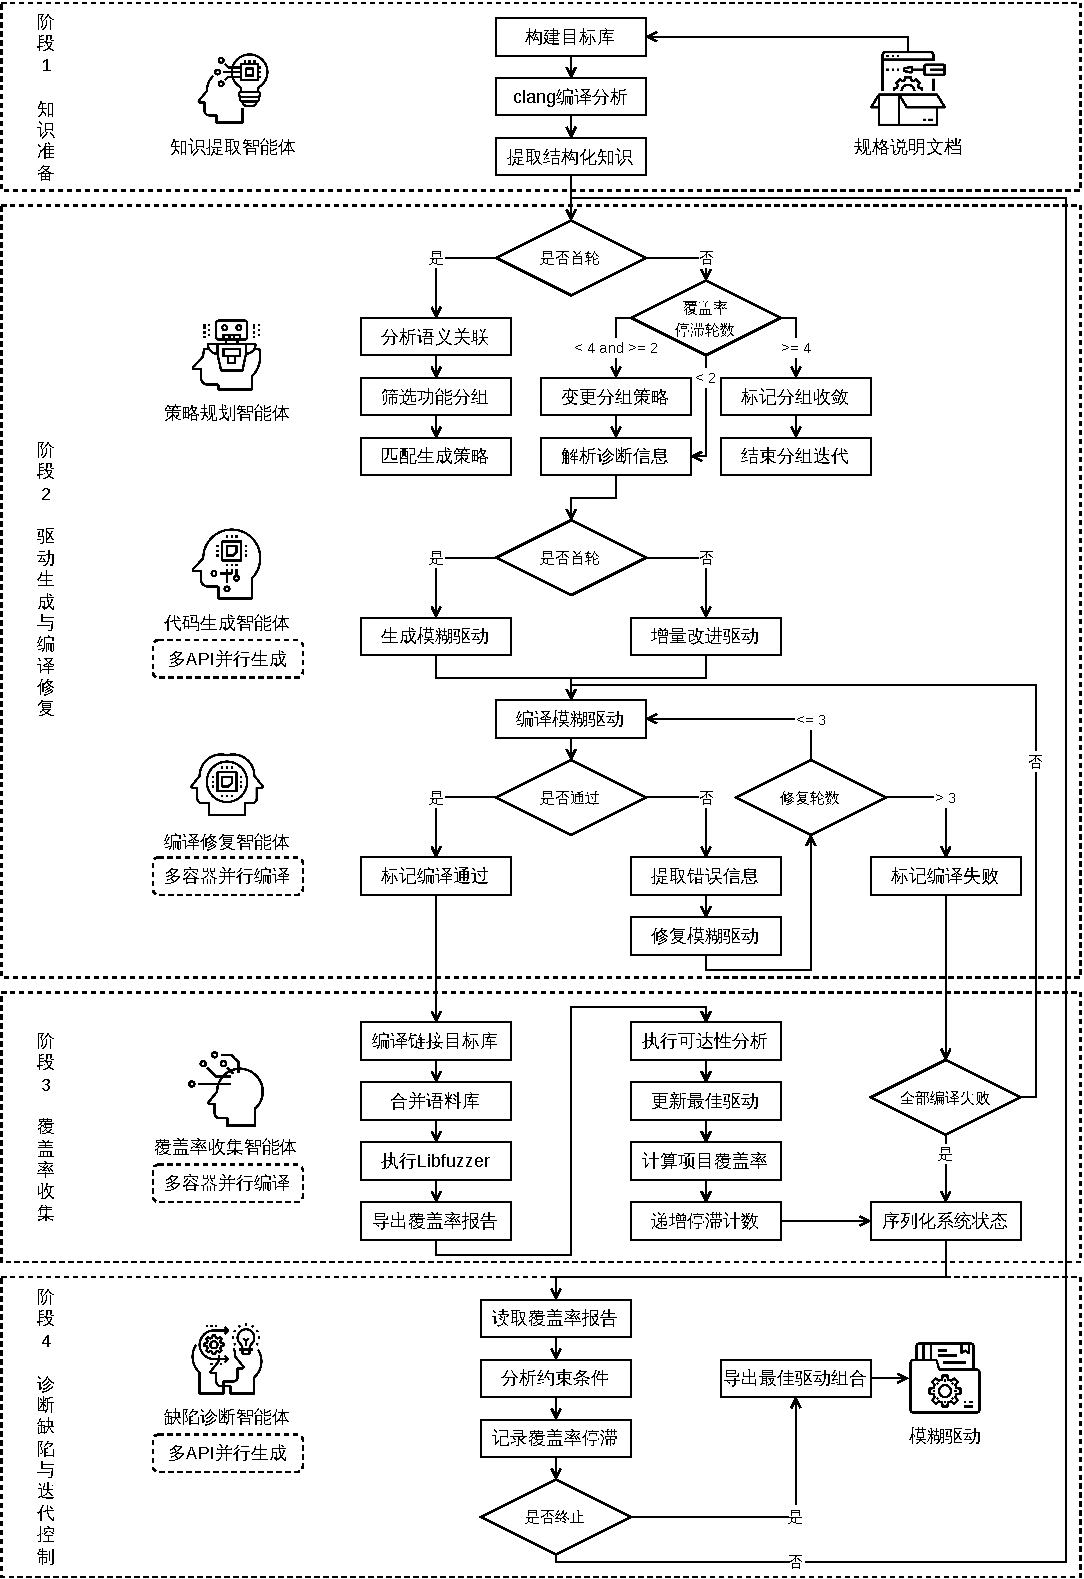
\includegraphics[width=\textwidth]{images/flowchart.drawio.pdf}}
    \caption{MAGIC4FDG系统整体流程图}
    \label{fig:flowchart}
\end{figure}

\textbf{知识准备阶段。}流水线的第一步交给知识提取智能体（Knowledge Agent）完成。该智能体先在Docker容器内编译目标库，随后借助clang前端执行AST导出。导出内容涵盖公开API的函数签名、参数类型与语义标注、函数间调用图，以及宏常量和枚举定义。值得一提的是，首次构建的产物会被缓存到宿主机上，后续轮次只需以只读方式挂载，省去重复编译的开销。整个知识准备仅在流水线启动时执行一次，其产出构成全局知识库，贯穿后续所有迭代轮次。

\textbf{驱动生成与编译修复阶段。}这个阶段涉及三个智能体的协作：策略规划（Planner Agent）、代码生成（Generation Agent）和编译修复（Patching Agent）。

策略规划智能体在知识提取完成后启动工作。首轮迭代属于探索阶段，它加载策略库里十种预定义策略的元数据，每种策略用结构化格式声明适用条件、最佳场景和不兼容约束，同时附带一段策略正文作为提示词后缀。智能体调用LLM分析目标库API之间的语义关系和功能分组，把策略元数据的适用条件跟API特征做匹配，给每个驱动槽位选一个最合适的策略。这里的关键在于，不同槽位会拿到完全不同的策略后缀，从而在代码生成环节产出风格迥异的驱动。如果LLM调用失败，系统回退到基于调用图的规则引擎做确定性匹配。到了后续轮次（利用阶段），策略规划智能体不再调LLM，而是根据各槽位的覆盖率停滞情况决定是否切换策略或标记收敛，同时从缺口诊断结果中提取额外的目标API补充到对应槽位的生成上下文里。

代码生成智能体根据规划结果并行生成驱动代码。它的提示由三部分拼接而成：基础模板（库名、接口规范、通用约束）、API知识上下文（目标API的签名、类型、调用关系）、策略提示词后缀（由Planner匹配的策略正文）。首轮是从零生成，LLM基于这三部分合成完整驱动；后续轮次是增量改进，提示里额外包含当前最佳代码、Analyst输出的结构化约束、以及跨轮次累积的经验知识，要求模型保留已有覆盖路径并定向扩展新路径。

编译修复智能体对所有生成的变体做编译验证和错误修复。每个变体在Docker容器内用带ASan插桩的方式编译，跟目标库静态链接。编译通过则标记成功；未通过的，提取编译器报错，将代码和错误信息注入修复提示模板由LLM修复，最多尝试三次。

编译修复完成后，系统做第一个条件路由判断，只要有至少一个变体编译通过，就进入下一阶段；如果全部失败，则跳过模糊测试直接进入状态持久化，避免无效执行。

\textbf{模糊测试与覆盖率收集阶段。}覆盖率收集智能体（Coverage Agent）负责跑模糊测试并收集精确的覆盖率数据。对每个编译通过的变体，它在Docker容器里依次做这几件事：先用覆盖率插桩标志重新编译驱动并链接目标库；然后合并种子语料库和历史累积语料库，以LibFuzzer的fork模式跑模糊测试。fork模式让每个输入在独立子进程里执行，某个输入触发崩溃不会终止整个测试进程；测试结束后通过语料库重放收集完整覆盖率数据（fork模式下profraw可能写不完整，因此需要重放一遍）；最后用LLVM工具链合并原始数据并导出行级与分支级覆盖率报告。另外，这个智能体还会做控制流图可达性分析，把结构上不可达的代码行标记出来，免得后面Analyst在这些行上浪费精力。覆盖率收集完毕后，系统逐槽位比对本轮与历史最佳覆盖率。若有提升则替换最佳版本，否则将该槽位的停滞计数加一。项目级覆盖率取所有槽位覆盖行的并集。

随后流水线进入状态持久化节点（Checkpoint Node）。这一节点不涉及LLM调用，职责单一，即把当前完整的流水线状态（含各变体源码）序列化为检查点文件写入磁盘。有了这份快照，用户可以从任意已完成的轮次恢复执行。

\textbf{缺口诊断与迭代控制阶段。}这一阶段由Analyst Agent主导。它逐一审视每个活跃槽位的覆盖率缺口，尝试定位根因。具体做法是：读取该槽位当前最佳代码、未覆盖行列表和函数级覆盖率数据，连同API知识上下文一并注入分析提示模板，交由LLM完成诊断。LLM返回的是结构化结果，输出分为三部分：约束列表（要触发某个分支需满足的前置条件）、未覆盖代码簇（按功能分组的未覆盖区域）、以及新发现的知识点。这些内容会追加到该槽位自身的知识空间里，轮次之间持续累积，使系统在迭代中逐步加深对目标库的理解。

Analyst完成分析后，系统做第二个条件路由判断，检查四个终止条件：项目级覆盖率达到用户设定的目标、迭代轮次到上限、所有槽位都已收敛、或者项目级覆盖率连续多轮没有明显提升。满足任何一个就终止迭代，输出各槽位的最佳版本并生成实验报告；否则回到策略规划智能体开始新一轮，进入利用阶段的闭环优化。

\section{需求分析}

MAGIC4FDG的核心功能是为C/C++开源库自动生成高质量模糊驱动，并通过覆盖率反馈迭代持续优化。除此之外，系统还需具备可扩展性、可靠性、可恢复性等非功能性需求。下面从涉众分析出发，明确谁会使用本系统、他们关心什么，再逐一梳理功能性和非功能性需求，最后给出用例图和用例描述。

\subsection{涉众分析}

根据技术背景和使用目的的不同，MAGIC4FDG系统的涉众可以分为三类：目标项目开发者、模糊测试使用者和模糊测试研究人员。表\ref{tab:stakeholder}列出了这三类涉众的特征和期望。

\begin{table}[H]
    \centering
    \caption{涉众分析结果}
    \makebox[\textwidth]{
    \begin{tabular}{ |c|p{5.2cm}|p{5.2cm}| }
        \hline
        \textbf{涉众名称} & \textbf{涉众特征} & \textbf{涉众期望} \\
        \hline
        \textbf{目标项目开发者} &
        被选为测试对象的开源项目的维护者，通常具备较强的C/C++工程能力，熟悉自身接口设计与使用语义，了解模糊测试平台的基本要求。该类涉众直接参与项目构建与接口演进，对系统产出的驱动可用性与行为一致性有要求。 &
        希望系统能够在不破坏接口契约的前提下，自动生成结构完整、逻辑合理、覆盖真实调用路径的模糊测试驱动，用于集成测试、安全审计或接口验证，降低人工编写负担并提高测试质量。 \\
        \hline
        \textbf{模糊测试使用者} &
        使用LibFuzzer、AFL或OSS-Fuzz等平台执行模糊测试的测试工程师或安全研究人员，关注模糊驱动的适配性与执行效果。该类涉众具备模糊测试实践经验，熟悉驱动编写规范与覆盖率评估方法，但不一定深入了解目标库的内部实现。 &
        希望系统生成的驱动能够直接用于主流模糊测试引擎，具备较高的代码覆盖率和缺陷发现能力；同时期望系统提供覆盖率报告和迭代过程记录，便于评估测试效果和定位潜在漏洞。 \\
        \hline
        \textbf{模糊测试研究人员} &
        从事模糊测试自动化、驱动生成或大语言模型辅助测试等方向研究的学者或研究工程师。该类涉众关注系统的技术方法与创新点，通常将本系统与其他工具进行对比实验以验证方法的有效性。 &
        希望系统具备良好的可复现性和可配置性，能够在不同目标库上稳定运行；同时期望系统提供详细的实验数据（覆盖率变化曲线、迭代轮次统计、消融实验支持等），便于进行公平的横向对比和方法分析。 \\
        \hline
    \end{tabular}}
    \label{tab:stakeholder}
\end{table}

三类涉众的差异主要体现在技术背景和关注重点上。目标项目开发者关注驱动是否符合API使用规范及缺陷发现能力；模糊测试使用者关注覆盖率、崩溃数量及与现有测试基础设施的兼容性；模糊测试研究人员则更关注实验数据和配置灵活性。三者共同期望系统能够在减少人工干预的同时保证驱动质量。

\subsection{功能性需求分析}

在调研现有工具的基础上，本文梳理出七个方面的功能性需求：目标库配置与知识提取、策略规划与驱动生成、编译修复、模糊测试与覆盖率收集、缺口诊断与迭代优化、状态持久化与恢复、实验报告生成。具体内容见表\ref{tab:functional-req}。

\begin{table}[H]
    \centering
    \caption{功能性需求列表}
    \label{tab:functional-req}
    \makebox[\textwidth]{
    \begin{tabular}{ |c|p{3.8cm}|p{8cm}| }
        \hline
        \textbf{需求编号} & \textbf{需求名称} & \textbf{需求描述} \\
        \hline
        \textbf{R1} & 目标库配置与知识提取 & 用户可以通过配置文件指定目标C/C++库的构建方式、头文件路径和静态库路径，系统自动在Docker容器内完成构建并提取API知识 \\
        \hline
        \textbf{R2} & 策略规划与驱动生成 & 系统应能够根据目标库的API特征自动匹配合适的模糊策略，并基于策略指导生成多个风格互补的模糊驱动代码 \\
        \hline
        \textbf{R3} & 编译修复 & 系统应能够对生成的驱动代码执行编译验证，对编译失败的变体自动诊断错误原因并尝试修复 \\
        \hline
        \textbf{R4} & 模糊测试执行 & 系统应能够对编译成功的驱动在隔离环境中执行模糊测试，支持崩溃隔离和语料库累积 \\
        \hline
        \textbf{R5} & 覆盖率收集与分析 & 系统应能够收集行级与分支级覆盖率数据，执行可达性分析过滤不可达代码，并维护每个驱动的最佳版本记录 \\
        \hline
        \textbf{R6} & 缺口诊断与迭代优化 & 系统应能够对覆盖率缺口进行根因分析，输出结构化约束描述，并基于分析结果在后续轮次中定向改进驱动代码 \\
        \hline
        \textbf{R7} & 状态持久化与恢复 & 系统应能够在每轮迭代后保存完整的流水线状态，支持从任意检查点恢复执行 \\
        \hline
        \textbf{R8} & 实验报告生成 & 系统应能够在迭代结束后生成包含覆盖率统计、迭代历史和最佳驱动代码的实验报告 \\
        \hline
    \end{tabular}}
\end{table}

目标库配置与知识提取（R1）是一切的起点。用户编写一个JSON配置文件，将库名、构建命令、头文件路径、静态库路径等信息填入即可。系统拿到配置后在Docker里编译目标库，然后用clang AST导出拿到结构化的API知识，包括函数签名、参数类型、调用图、宏常量等。这步的产出是一个全局知识库，后续所有智能体都从这里获取信息。

策略规划与驱动生成（R2）是整个系统最核心的部分。规划环节分析API的特征和适合的测试策略，然后给每个槽位分配一个；生成环节拿着分配好的策略后缀、API知识和基础模板去调LLM，让它写出完整的模糊驱动代码。第一轮从零开始写，后续轮次则在已有代码上做增量改进。

编译修复（R3）的目的很直接——保证代码能编译通过。变体逐个送入Docker容器，以带ASan插桩的方式编译并与目标库静态链接。编译未通过时，系统提取编译器报错交给LLM尝试修复，上限三次，超过即放弃。之所以设定三次而非更多，是在修复成本与收益之间做的权衡——实践中绝大多数可修复的错误在前两轮就能解决，第三轮仍失败的往往涉及设计层面的问题。保住尽可能多的变体，后续模糊测试才有足够的样本量。

模糊测试执行（R4）与覆盖率收集与分析（R5）共同构成测试与反馈环节。前者在Docker容器内以fork模式运行LibFuzzer，每个输入在独立子进程中执行，单个崩溃不会拖垮整体测试进程。后者负责精确度量，通过语料库重放（非fork模式）配合LLVM工具链，导出行级与分支级覆盖率数据。此外，系统还执行控制流图可达性分析，将结构上不可达的代码行预先标记，避免后续诊断环节在这些行上做无用功。

缺口诊断与迭代优化（R6）是覆盖率能够持续攀升的关键所在。Analyst针对每个槽位的未覆盖代码做根因分析，产出两类结构化信息：约束列表（触发特定分支所需的前置条件）和未覆盖代码簇（按功能聚类的未覆盖区域）。这些信息被写入各槽位独立的知识空间，轮次间不断累积。到了后续迭代，Generation Agent读取这些约束作为增量改进的精确指引，相当于把"哪里没覆盖、为什么没覆盖"的诊断结论直接转化为生成指令。

状态持久化与恢复（R7）保障容错能力。每轮迭代完成后，系统把完整的流水线状态序列化为检查点文件，包括所有槽位的最佳代码、覆盖率数据、累积知识和迭代计数。异常中断时用户可以指定检查点恢复执行，无需从头开始。

实验报告生成（R8）满足用户对结果的查阅需求。迭代终止后系统自动生成包含项目级覆盖率统计、各槽位覆盖率对比、迭代历史和最佳驱动源码的结构化报告，方便评估效果和做横向对比。

\subsection{非功能性需求分析}

功能性需求之外，非功能性需求同样重要。本文将其分为质量属性、性能需求和约束三部分，具体见表\ref{tab:nonfunctional-req}。

\begin{table}[H]
    \centering
    \caption{非功能性需求列表}
    \label{tab:nonfunctional-req}
    \makebox[\textwidth]{
    \begin{tabular}{ |c|c|p{3cm}|p{7cm}| }
        \hline
        \textbf{需求编号} & \textbf{需求类型} & \textbf{需求名称} & \textbf{需求描述} \\
        \hline
        \textbf{QA1} & 质量属性 & 可扩展性 & 系统应支持通过配置文件接入新的目标库，无需修改系统源码 \\
        \hline
        \textbf{QA2} & 质量属性 & 可靠性 & 系统生成的驱动在经过编译修复后应达到60\%以上的编译通过率 \\
        \hline
        \textbf{QA3} & 质量属性 & 可恢复性 & 系统应支持从任意轮次的检查点恢复执行，恢复后状态与中断前一致 \\
        \hline
        \textbf{QA4} & 质量属性 & 隔离性 & 所有编译、模糊测试和覆盖率收集操作应在Docker容器内执行，不影响宿主机环境 \\
        \hline
        \textbf{QA5} & 质量属性 & 可复现性 & 在相同配置和相同大语言模型下，系统的覆盖率结果应具备统计意义上的可复现性 \\
        \hline
        \textbf{PR1} & 性能需求 & 并行处理能力 & 系统应支持多个驱动变体的并行生成、并行编译和并行模糊测试 \\
        \hline
        \textbf{PR2} & 性能需求 & 构建缓存 & 目标库首次构建后应缓存产物，后续轮次的编译和模糊测试应复用缓存，避免重复构建 \\
        \hline
        \textbf{CS1} & 约束 & 开发语言 & 系统使用Python语言进行开发 \\
        \hline
        \textbf{CS2} & 约束 & 容器化依赖 & 系统运行依赖Docker引擎和LLVM工具链 \\
        \hline
    \end{tabular}}
\end{table}

质量属性方面本文列出五条，其中最重要的两条是可扩展性（QA1）和隔离性（QA4）。可扩展性的含义是，用户更换目标库时只需修改配置文件，系统代码本身不动。这一点直接决定了系统能否脱离实验室环境、真正被他人使用。隔离性则依赖Docker容器化来兑现，构建、模糊测试均在容器内完成，宿主机环境不受影响，多个库并行运行时也彼此隔离。可靠性（QA2）要求编译修复环节切实有效，每轮需保证足够数量的变体编译通过，否则后续测试无从谈起。可恢复性（QA3）通过检查点机制实现，中断后从最近的检查点恢复即可继续。可复现性（QA5）是实验评估的基本前提，本文通过固定随机种子与确定性调度两项措施加以保障。

性能需求方面，系统需要在代码生成、编译修复和模糊测试三个环节支持多变体并行执行（PR1）。这三个环节的计算相互独立，并行化能显著缩短单轮迭代耗时，充分利用多核资源。构建缓存（PR2）则要求目标库的编译产物在首次构建后持久化存储，后续轮次一律通过只读挂载复用，杜绝每轮重复构建带来的时间浪费。

约束方面，系统用Python开发（CS1），利用其丰富的生态支持LLM调用和流水线编排；运行依赖Docker引擎提供容器化执行环境，依赖LLVM工具链提供覆盖率插桩和数据导出能力（CS2）。

\subsection{系统用例图}

基于前面的涉众分析和功能性需求，本文对相关描述进行了实体识别、用例拆分和筛选，构建了系统用例图，如图\ref{fig:usecase}所示。

系统包含10个用例：配置目标库、提取API知识、规划模糊策略、生成模糊驱动、修复编译错误、执行模糊测试、收集覆盖率数据、诊断覆盖率缺口、恢复中断任务、查看实验报告。参与者有五类：三类人类参与者（目标项目开发者、模糊测试使用者、模糊测试研究人员）和两类外部系统参与者（Docker引擎、大语言模型服务）。

三类人类参与者都可以使用配置目标库、恢复中断任务和查看实验报告。提取API知识、规划模糊策略、生成模糊驱动、修复编译错误、执行模糊测试、收集覆盖率数据和诊断覆盖率缺口这七个用例是系统内部自动执行的流程，用户启动任务后由系统自动编排。Docker引擎参与知识提取、编译修复、模糊测试和覆盖率收集四个用例；大语言模型服务参与策略规划、驱动生成、编译修复和缺口诊断四个用例。

\begin{figure}[H]
    \centering
    \makebox[\textwidth]{
    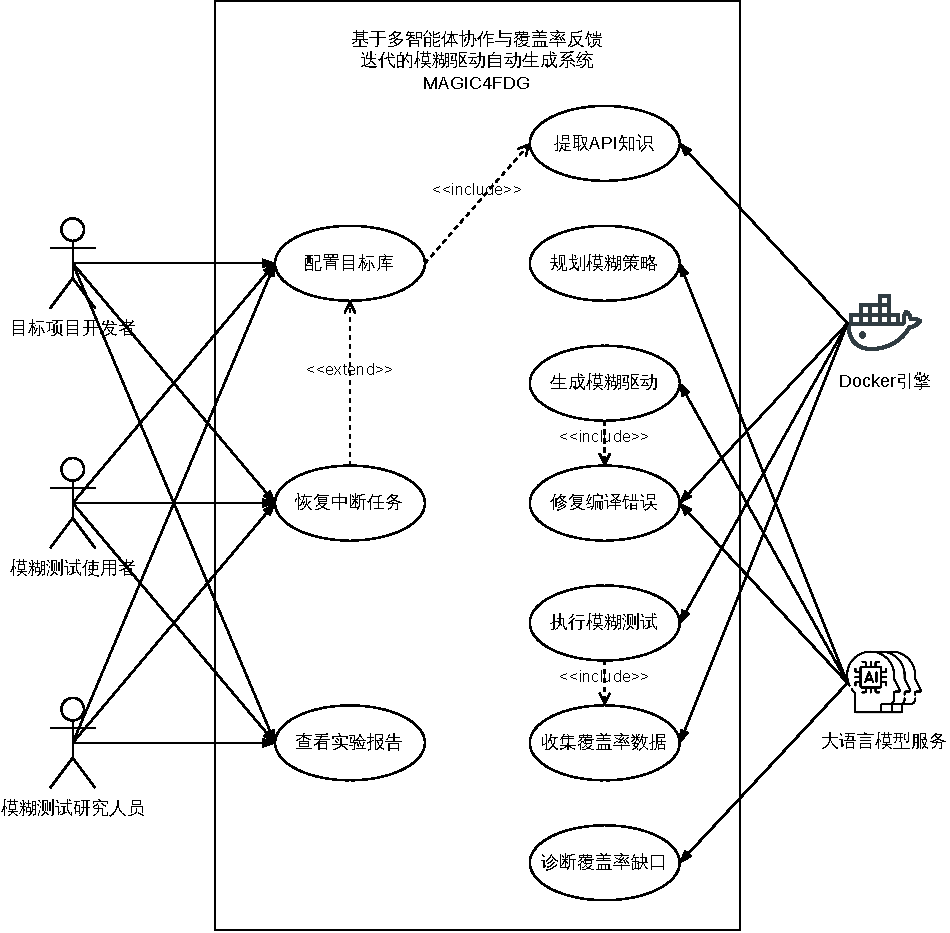
\includegraphics[width=\textwidth]{images/usecase.drawio.pdf}}
    \caption{MAGIC4FDG系统用例图}
    \label{fig:usecase}
\end{figure}

\subsection{系统用例描述}

上面的用例图从用户视角展示了系统行为与需求之间的关系。下面逐一描述每个用例的细节，帮助理解系统功能并指导后续设计。

配置目标库是用户使用系统的入口。用户编写JSON配置文件声明目标库的构建方式和路径信息，通过命令行参数控制迭代轮次、目标覆盖率等运行时行为，系统据此启动自动化流程。表\ref{tab:uc1}是该用例的详细描述。

\begin{table}[H]
    \centering
    \caption{用例"配置目标库"详细描述}
    \label{tab:uc1}
    \makebox[\textwidth]{
    \begin{tabular}{ |c|p{12cm}| }
        \hline
        \textbf{用例编号} & UC1 \\
        \hline
        \textbf{用例名称} & 配置目标库 \\
        \hline
        \textbf{参与者} & 目标项目开发者、模糊测试使用者、模糊测试研究人员 \\
        \hline
        \textbf{前置条件} & 目标库源码可通过网络获取，用户了解目标库的构建方式 \\
        \hline
        \textbf{后置条件} & 系统获得有效的目标库配置，可启动自动化生成流程 \\
        \hline
        \textbf{基本流程} &
        1. 用户编写目标库配置文件，指定库名、构建命令、头文件路径、静态库路径和覆盖率源文件路径 \newline
        2. 用户通过命令行指定配置文件路径和运行参数（最大轮次、目标覆盖率、模糊测试时长等） \newline
        3. 系统验证配置文件格式和必填字段的完整性 \newline
        4. 系统启动流水线执行 \\
        \hline
        \textbf{扩展流程} & 3a. 配置文件格式错误或缺少必填字段时，系统输出错误提示并终止 \\
        \hline
    \end{tabular}}
\end{table}

提取API知识是获取目标库结构化信息的基础操作。系统利用clang前端的AST导出能力，在Docker容器内精确提取函数签名、参数类型、调用图和宏常量定义，构建产物缓存到宿主机避免后续重复构建。表\ref{tab:uc2}是该用例的详细描述。

\begin{table}[H]
    \centering
    \caption{用例"提取API知识"详细描述}
    \label{tab:uc2}
    \begin{tabular}{ |c|p{12cm}| }
        \hline
        \textbf{用例编号} & UC2 \\
        \hline
        \textbf{用例名称} & 提取API知识 \\
        \hline
        \textbf{参与者} & Docker引擎 \\
        \hline
        \textbf{前置条件} & 系统获得有效的目标库配置 \\
        \hline
        \textbf{后置条件} & 系统获得目标库的结构化API知识（函数签名、调用图、类型信息） \\
        \hline
        \textbf{基本流程} &
        1. 系统在Docker容器内执行目标库的构建命令 \newline
        2. 系统通过clang AST导出提取头文件和源文件中的API信息 \newline
        3. 系统解析AST JSON，提取函数签名、参数类型、调用图和宏定义 \newline
        4. 系统将构建产物缓存至宿主机 \newline
        5. 系统将提取结果存入全局知识库 \\
        \hline
        \textbf{扩展流程} & 1a. 构建失败时，系统输出构建日志并终止流程 \\
        \hline
    \end{tabular}
\end{table}

规划模糊策略是为每个槽位选择最合适生成策略的决策环节。探索阶段，Planner通过LLM把策略库中十种策略与目标库API特征做匹配；利用阶段，根据覆盖率停滞情况动态调整策略分配。表\ref{tab:uc3}是该用例的详细描述。

\begin{table}[H]
    \centering
    \caption{用例"规划模糊策略"详细描述}
    \label{tab:uc3}
    \begin{tabular}{ |c|p{12cm}| }
        \hline
        \textbf{用例编号} & UC3 \\
        \hline
        \textbf{用例名称} & 规划模糊策略 \\
        \hline
        \textbf{参与者} & 大语言模型服务 \\
        \hline
        \textbf{前置条件} & 系统已完成API知识提取 \\
        \hline
        \textbf{后置条件} & 每个模糊驱动获得匹配的生成策略和目标API列表 \\
        \hline
        \textbf{基本流程} &
        1. 系统加载策略库中十种模糊策略的元数据 \newline
        2. 系统将API知识注入规划提示模板 \newline
        3. 系统调用大语言模型分析API语义关系并匹配策略 \newline
        4. 系统为每个模糊驱动分配目标API和对应策略 \\
        \hline
        \textbf{扩展流程} & 3a. 大语言模型调用失败时，系统回退至基于调用图的规则引擎进行确定性匹配 \\
        \hline
    \end{tabular}
\end{table}

生成模糊驱动是核心的代码生成环节。每个槽位接收差异化的策略后缀，引导LLM采用不同的代码结构和API调用模式；首轮从零生成，后续轮次切换为基于约束和累积经验的增量改进。表\ref{tab:uc4}是该用例的详细描述。

\begin{table}[H]
    \centering
    \caption{用例"生成模糊驱动"详细描述}
    \label{tab:uc4}
    \begin{tabular}{ |c|p{12cm}| }
        \hline
        \textbf{用例编号} & UC4 \\
        \hline
        \textbf{用例名称} & 生成模糊驱动 \\
        \hline
        \textbf{参与者} & 大语言模型服务 \\
        \hline
        \textbf{前置条件} & 策略规划完成，每个驱动已分配目标API和策略 \\
        \hline
        \textbf{后置条件} & 系统获得多个模糊驱动代码变体 \\
        \hline
        \textbf{基本流程} &
        1. 系统为每个驱动组装提示（基础模板+API知识+策略后缀） \newline
        2. 系统并行调用大语言模型生成驱动代码 \newline
        3. 系统从模型输出中提取代码块并保存为变体文件 \\
        \hline
        \textbf{扩展流程} & 2a. 后续轮次，提示额外包含最佳代码、约束列表和累积经验 \\
        \hline
    \end{tabular}
\end{table}

修复编译错误保证生成的代码能通过编译。编译修复智能体在Docker容器内做带ASan插桩的编译，失败的变体提取错误信息让LLM修复，最多三次。表\ref{tab:uc5}是该用例的详细描述。

\begin{table}[H]
    \centering
    \caption{用例"修复编译错误"详细描述}
    \label{tab:uc5}
    \begin{tabular}{ |c|p{12cm}| }
        \hline
        \textbf{用例编号} & UC5 \\
        \hline
        \textbf{用例名称} & 修复编译错误 \\
        \hline
        \textbf{参与者} & Docker引擎、大语言模型服务 \\
        \hline
        \textbf{前置条件} & 代码生成智能体已输出驱动变体 \\
        \hline
        \textbf{后置条件} & 变体被标记为编译成功或编译失败（已耗尽重试次数） \\
        \hline
        \textbf{基本流程} &
        1. 系统在Docker容器内对变体执行带插桩的编译 \newline
        2. 编译成功，标记变体为通过 \\
        \hline
        \textbf{扩展流程} &
        1a. 编译失败时，系统提取错误信息并调用大语言模型生成修复代码 \newline
        1b. 重新编译修复后的代码，最多重试三次 \newline
        1c. 三次重试均失败，标记变体为编译失败 \\
        \hline
    \end{tabular}
\end{table}

执行模糊测试是对目标库做自动化安全测试的核心环节。fork模式让每个输入在独立子进程里跑，单个崩溃不会终止整个测试；每轮发现的有效输入持久化存储供后续轮次复用。表\ref{tab:uc6}是该用例的详细描述。

\begin{table}[H]
    \centering
    \caption{用例"执行模糊测试"详细描述}
    \label{tab:uc6}
    \begin{tabular}{ |c|p{12cm}| }
        \hline
        \textbf{用例编号} & UC6 \\
        \hline
        \textbf{用例名称} & 执行模糊测试 \\
        \hline
        \textbf{参与者} & Docker引擎 \\
        \hline
        \textbf{前置条件} & 存在至少一个编译成功的驱动变体 \\
        \hline
        \textbf{后置条件} & 系统获得模糊测试产生的语料库和崩溃样本 \\
        \hline
        \textbf{基本流程} &
        1. 系统以覆盖率插桩标志重新编译驱动变体 \newline
        2. 系统合并种子语料库与历史累积语料库 \newline
        3. 系统以fork模式运行LibFuzzer执行模糊测试 \newline
        4. 系统收集测试产生的新语料库和崩溃样本 \\
        \hline
        \textbf{扩展流程} & 3a. 所有变体均编译失败时，跳过本用例直接进入状态持久化 \\
        \hline
    \end{tabular}
\end{table}

收集覆盖率数据是获取精确反馈的关键环节。fork模式下profraw文件可能写不完整，所以系统通过语料库重放在非fork模式下重新执行所有输入来保证数据完整性，同时维护每个槽位的最佳版本记录和停滞计数。表\ref{tab:uc7}是该用例的详细描述。

\begin{table}[H]
    \centering
    \caption{用例"收集覆盖率数据"详细描述}
    \label{tab:uc7}
    \begin{tabular}{ |c|p{12cm}| }
        \hline
        \textbf{用例编号} & UC7 \\
        \hline
        \textbf{用例名称} & 收集覆盖率数据 \\
        \hline
        \textbf{参与者} & Docker引擎 \\
        \hline
        \textbf{前置条件} & 模糊测试执行完成，语料库已生成 \\
        \hline
        \textbf{后置条件} & 系统获得行级与分支级覆盖率报告，最佳版本记录已更新 \\
        \hline
        \textbf{基本流程} &
        1. 系统通过语料库重放机制收集完整的覆盖率原始数据 \newline
        2. 系统通过LLVM工具链合并数据并导出覆盖率报告 \newline
        3. 系统执行控制流图可达性分析，标记不可达代码行 \newline
        4. 系统比较当前覆盖率与历史最佳，更新最佳版本记录 \newline
        5. 系统计算项目级覆盖率并更新停滞计数 \\
        \hline
        \textbf{扩展流程} & 4a. 当前覆盖率未超过历史最佳时，递增该驱动的停滞计数 \\
        \hline
    \end{tabular}
\end{table}

诊断覆盖率缺口是实现精准迭代改进的智能分析环节。Analyst只输出结构化的约束描述和未覆盖代码簇分析，把"诊断"和"生成"的职责分开；诊断结果持久化到每个槽位的隔离知识空间，跨轮次累积形成经验库。表\ref{tab:uc8}是该用例的详细描述。

\begin{table}[H]
    \centering
    \caption{用例"诊断覆盖率缺口"详细描述}
    \label{tab:uc8}
    \begin{tabular}{ |c|p{12cm}| }
        \hline
        \textbf{用例编号} & UC8 \\
        \hline
        \textbf{用例名称} & 诊断覆盖率缺口 \\
        \hline
        \textbf{参与者} & 大语言模型服务 \\
        \hline
        \textbf{前置条件} & 覆盖率数据收集完成 \\
        \hline
        \textbf{后置条件} & 每个活跃驱动获得结构化的约束列表和未覆盖代码簇分析 \\
        \hline
        \textbf{基本流程} &
        1. 系统读取每个驱动的最佳代码和未覆盖代码行列表 \newline
        2. 系统将覆盖率数据与API知识注入分析提示模板 \newline
        3. 系统调用大语言模型进行根因分析 \newline
        4. 系统将输出的约束和知识追加到驱动的隔离知识空间 \\
        \hline
        \textbf{扩展流程} & 3a. 大语言模型输出格式异常时，系统跳过该驱动的本轮分析 \\
        \hline
    \end{tabular}
\end{table}

恢复中断任务让用户能从之前保存的检查点继续执行。MAGIC4FDG的单次完整运行可能持续数小时（取决于目标库复杂度、迭代轮次和模糊测试时长），期间可能因网络波动、LLM服务不可用或系统资源不足而中断。检查点恢复机制确保用户无需从头开始，可以从最近一次成功完成的轮次继续。表\ref{tab:uc9}是该用例的详细描述。

\begin{table}[H]
    \centering
    \caption{用例"恢复中断任务"详细描述}
    \label{tab:uc9}
    \begin{tabular}{ |c|p{12cm}| }
        \hline
        \textbf{用例编号} & UC9 \\
        \hline
        \textbf{用例名称} & 恢复中断任务 \\
        \hline
        \textbf{参与者} & 目标项目开发者、模糊测试使用者、模糊测试研究人员 \\
        \hline
        \textbf{前置条件} & 系统存在之前保存的检查点文件 \\
        \hline
        \textbf{后置条件} & 系统从指定检查点恢复完整的流水线状态并继续迭代 \\
        \hline
        \textbf{基本流程} &
        1. 用户通过命令行参数指定检查点文件路径 \newline
        2. 系统反序列化检查点文件，恢复流水线状态 \newline
        3. 系统从恢复的轮次继续执行迭代流程 \\
        \hline
        \textbf{扩展流程} & 2a. 检查点文件损坏或格式不兼容时，系统输出报错并终止 \\
        \hline
    \end{tabular}
\end{table}

查看实验报告让用户了解系统的运行结果和测试效果。对三类涉众来说，报告是评估系统产出质量的主要途径——开发者通过它了解驱动覆盖了哪些API路径、发现了哪些缺陷；测试使用者通过它评估覆盖率水平和崩溃发现能力；研究人员通过其中的定量数据做横向对比。报告同时以Markdown和JSON两种格式输出，兼顾可读性和自动化处理需求。表\ref{tab:uc10}是该用例的详细描述。 

\begin{table}[H]
    \centering
    \caption{用例"查看实验报告"详细描述}
    \label{tab:uc10}
    \begin{tabular}{ |c|p{12cm}| }
        \hline
        \textbf{用例编号} & UC10 \\
        \hline
        \textbf{用例名称} & 查看实验报告 \\
        \hline
        \textbf{参与者} & 目标项目开发者、模糊测试使用者、模糊测试研究人员 \\
        \hline
        \textbf{前置条件} & 系统迭代终止（满足任一终止条件） \\
        \hline
        \textbf{后置条件} & 用户获得包含覆盖率统计和最佳驱动代码的结构化报告 \\
        \hline
        \textbf{基本流程} &
        1. 系统在迭代终止后自动生成Markdown和JSON格式的实验报告 \newline
        2. 报告包含项目级覆盖率、各驱动覆盖率对比、迭代历史和最佳驱动源码 \newline
        3. 用户查阅报告评估测试效果 \\
        \hline
        \textbf{扩展流程} & 1a. 用户可通过配置选择报告中包含的内容项 \\
        \hline
    \end{tabular}
\end{table}

\section{系统概要设计}

本节用"4+1"视图方法描述MAGIC4FDG的架构。"4+1"视图包含逻辑视图、开发视图、进程视图、物理视图和场景视图五部分，其中场景视图就是3.2节的用例视图，已经在需求分析阶段完成了。下面先介绍整体架构设计，再从模块划分、逻辑视图、开发视图、进程视图和物理视图四个维度展开。

\subsection{系统整体架构设计}

图\ref{fig:architecture}展示了MAGIC4FDG的整体架构。用户提供目标库配置后，系统在Docker容器内依次完成知识提取、驱动生成、编译修复、模糊测试与覆盖率收集、缺口诊断等环节。各环节的产出经由共享状态对象流转，形成迭代反馈闭环以持续优化覆盖率。图中按模块划分了系统功能，箭头标明模块间的依赖方向。

\begin{figure}[htbp]
    \centering
    \makebox[\textwidth]{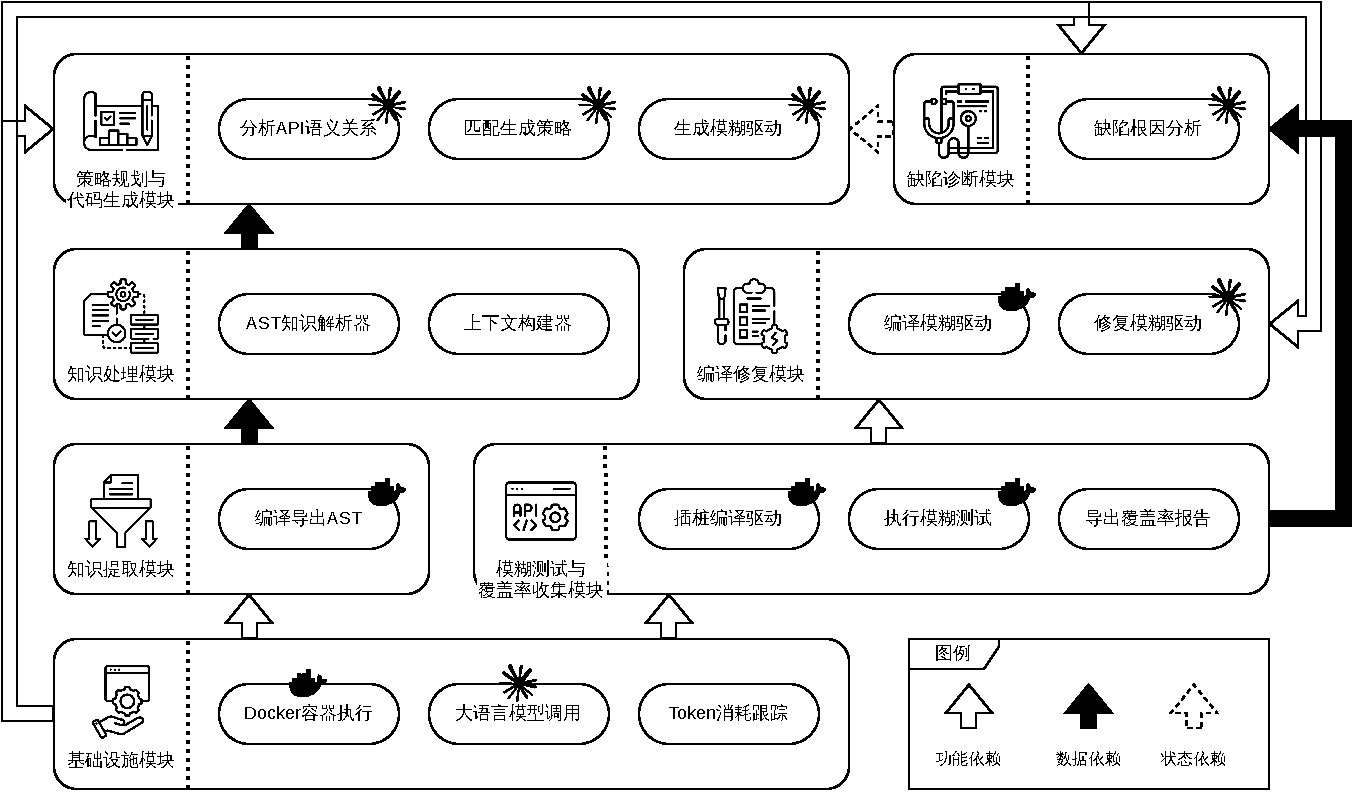
\includegraphics[width=1.1\textwidth]{images/architecture.drawio.pdf}}
    \caption{MAGIC4FDG系统整体架构图}
    \label{fig:architecture}
\end{figure}

架构自底向上分层，共包含七个功能模块，具体包括：基础设施、知识处理、知识提取、策略规划与代码生成、编译修复、模糊测试与覆盖率收集、缺口诊断。

基础设施模块是底座，提供Docker执行、LLM调用和令牌追踪三项服务，其他模块都依赖它。知识处理模块解析clang AST输出，将原始的语法树信息转换为各智能体能直接使用的文本片段。知识提取模块在Docker里编译目标库、做AST导出，产出全局知识库。策略规划与代码生成模块是核心，负责分析API语义、匹配策略、并行生成多个风格不同的驱动。编译修复模块负责将编译失败的变体修复。模糊测试与覆盖率收集模块执行测试、收集数据。缺口诊断模块分析哪里没覆盖到、为什么没覆盖到，输出约束供下一轮使用。各模块的详细设计在下一小节展开。

\subsection{系统模块划分}

在需求分析的基础上做模块化划分，可以有效降低系统复杂度，让结构更清晰。MAGIC4FDG按功能职责分为七个模块，下面逐一介绍，最后解释模块间的依赖关系。

\textbf{基础设施模块。}该模块并不直接对应某个功能性需求或用例，但它是其他所有模块赖以运行的技术底座。内部包含三个核心组件。其一，Docker执行器，封装知识提取、编译、模糊测试、覆盖率收集四类容器化操作的命令构建与执行逻辑，同时负责构建缓存的创建与挂载管理，对应QA4（隔离性）和PR2（构建缓存）两项非功能性需求。其二，LLM工厂，以统一接口创建带重试机制的模型客户端实例，集中管理配置参数、超时策略和错误处理。其三，令牌追踪器，按智能体类型分类记录每次模型调用的令牌消耗，供成本监控和实验分析使用。

\textbf{知识处理模块。}对应R1中的知识组织部分。三个组件各负责一项工作：提取器负责解析clang AST的JSON输出，从中提取函数签名、参数类型、调用图和宏常量；上下文构建器根据"谁要用"来决定"给什么"——代码生成智能体需要看目标API的完整签名和调用关系，Analyst需要看未覆盖代码行的上下文，同一份知识给不同智能体的视图是不一样的；分组引擎做基于调用图的API分组和规则引擎策略匹配，当LLM策略规划失败时作为确定性回退。

\textbf{知识提取模块。}对应R1和UC2。功能较为明确，即在Docker容器内编译目标库，用clang前端做AST导出，结果交给知识处理模块去解析。构建产物会缓存到宿主机，后续的编译和模糊测试容器只读挂载即可，无需每轮重新构建。该模块仅执行一次。

\textbf{策略规划与代码生成模块。}对应R2、UC3和UC4，是整个系统的核心。探索阶段加载十种策略的元数据，让LLM分析API之间的语义关系，给每个槽位匹配策略；然后用差异化的提示词并行生成多个驱动。利用阶段则根据覆盖率停滞情况动态调整策略，将Analyst的约束和历史经验注入提示词做增量改进。

\textbf{编译修复模块。}对应R3和UC5。对每个变体在Docker容器内做带ASan插桩的编译和静态链接。编译通过则标记成功；未通过的提取错误信息由LLM修复，最多三次。该模块的存在让系统对LLM代码生成质量有容错能力，保证每轮有足够变体进入模糊测试。

\textbf{模糊测试与覆盖率收集模块。}对应R4、R5、UC6和UC7。对每个编译通过的变体，在Docker容器内依次做：覆盖率插桩重编译、合并语料库、fork模式模糊测试、语料库重放收集完整覆盖率、LLVM工具链导出行级与分支级报告。还做控制流图可达性分析过滤不可达代码行，并维护各槽位的最佳版本记录和停滞计数。

\textbf{缺口诊断模块。}对应R6和UC8。对每个活跃槽位，读取最佳代码和未覆盖代码行列表，把覆盖率数据与API知识注入分析提示模板让LLM做根因分析。输出结构化的约束列表和未覆盖代码簇，追加到对应槽位的隔离知识空间，跨轮次累积，为后续的策略规划与代码生成提供精确的改进指导。

\textbf{模块之间的依赖关系。}图\ref{fig:architecture}的架构是基于需求分析得到的功能性需求和用例做模块化划分的结果，模块间存在数据依赖、功能依赖和状态依赖三类关系。整体上看，系统采用分层架构，上层依赖下层，下层不依赖上层，符合依赖倒置原则，有效降低了耦合度。

具体来说：知识提取模块对基础设施模块是功能依赖（调用Docker执行器在容器内完成构建和AST导出），对知识处理模块是数据依赖（调用提取器解析AST JSON并构建知识库）。策略规划与代码生成模块、缺口诊断模块对知识处理模块是数据依赖，它们需要知识处理模块提供的结构化API知识和格式化上下文文本。所有涉及LLM调用的模块对基础设施模块是功能依赖，基础设施模块提供LLM调用服务和Docker执行服务。编译修复模块和模糊测试与覆盖率收集模块对基础设施模块同样是功能依赖，都通过Docker执行器在容器内完成各自的工作。缺口诊断模块与策略规划与代码生成模块之间是状态依赖，Analyst的输出（约束列表和累积知识）通过共享的流水线状态对象传递给后者，后者在后续轮次中据此调整生成策略和提示词内容。

\subsection{系统逻辑视图}

逻辑视图关注功能性需求，描述系统的主要组件、类和它们之间的关系，通常用类图表示。图\ref{fig:logic-view}是MAGIC4FDG的逻辑视图。

\begin{figure}[htbp]
    \centering
    \makebox[\textwidth]{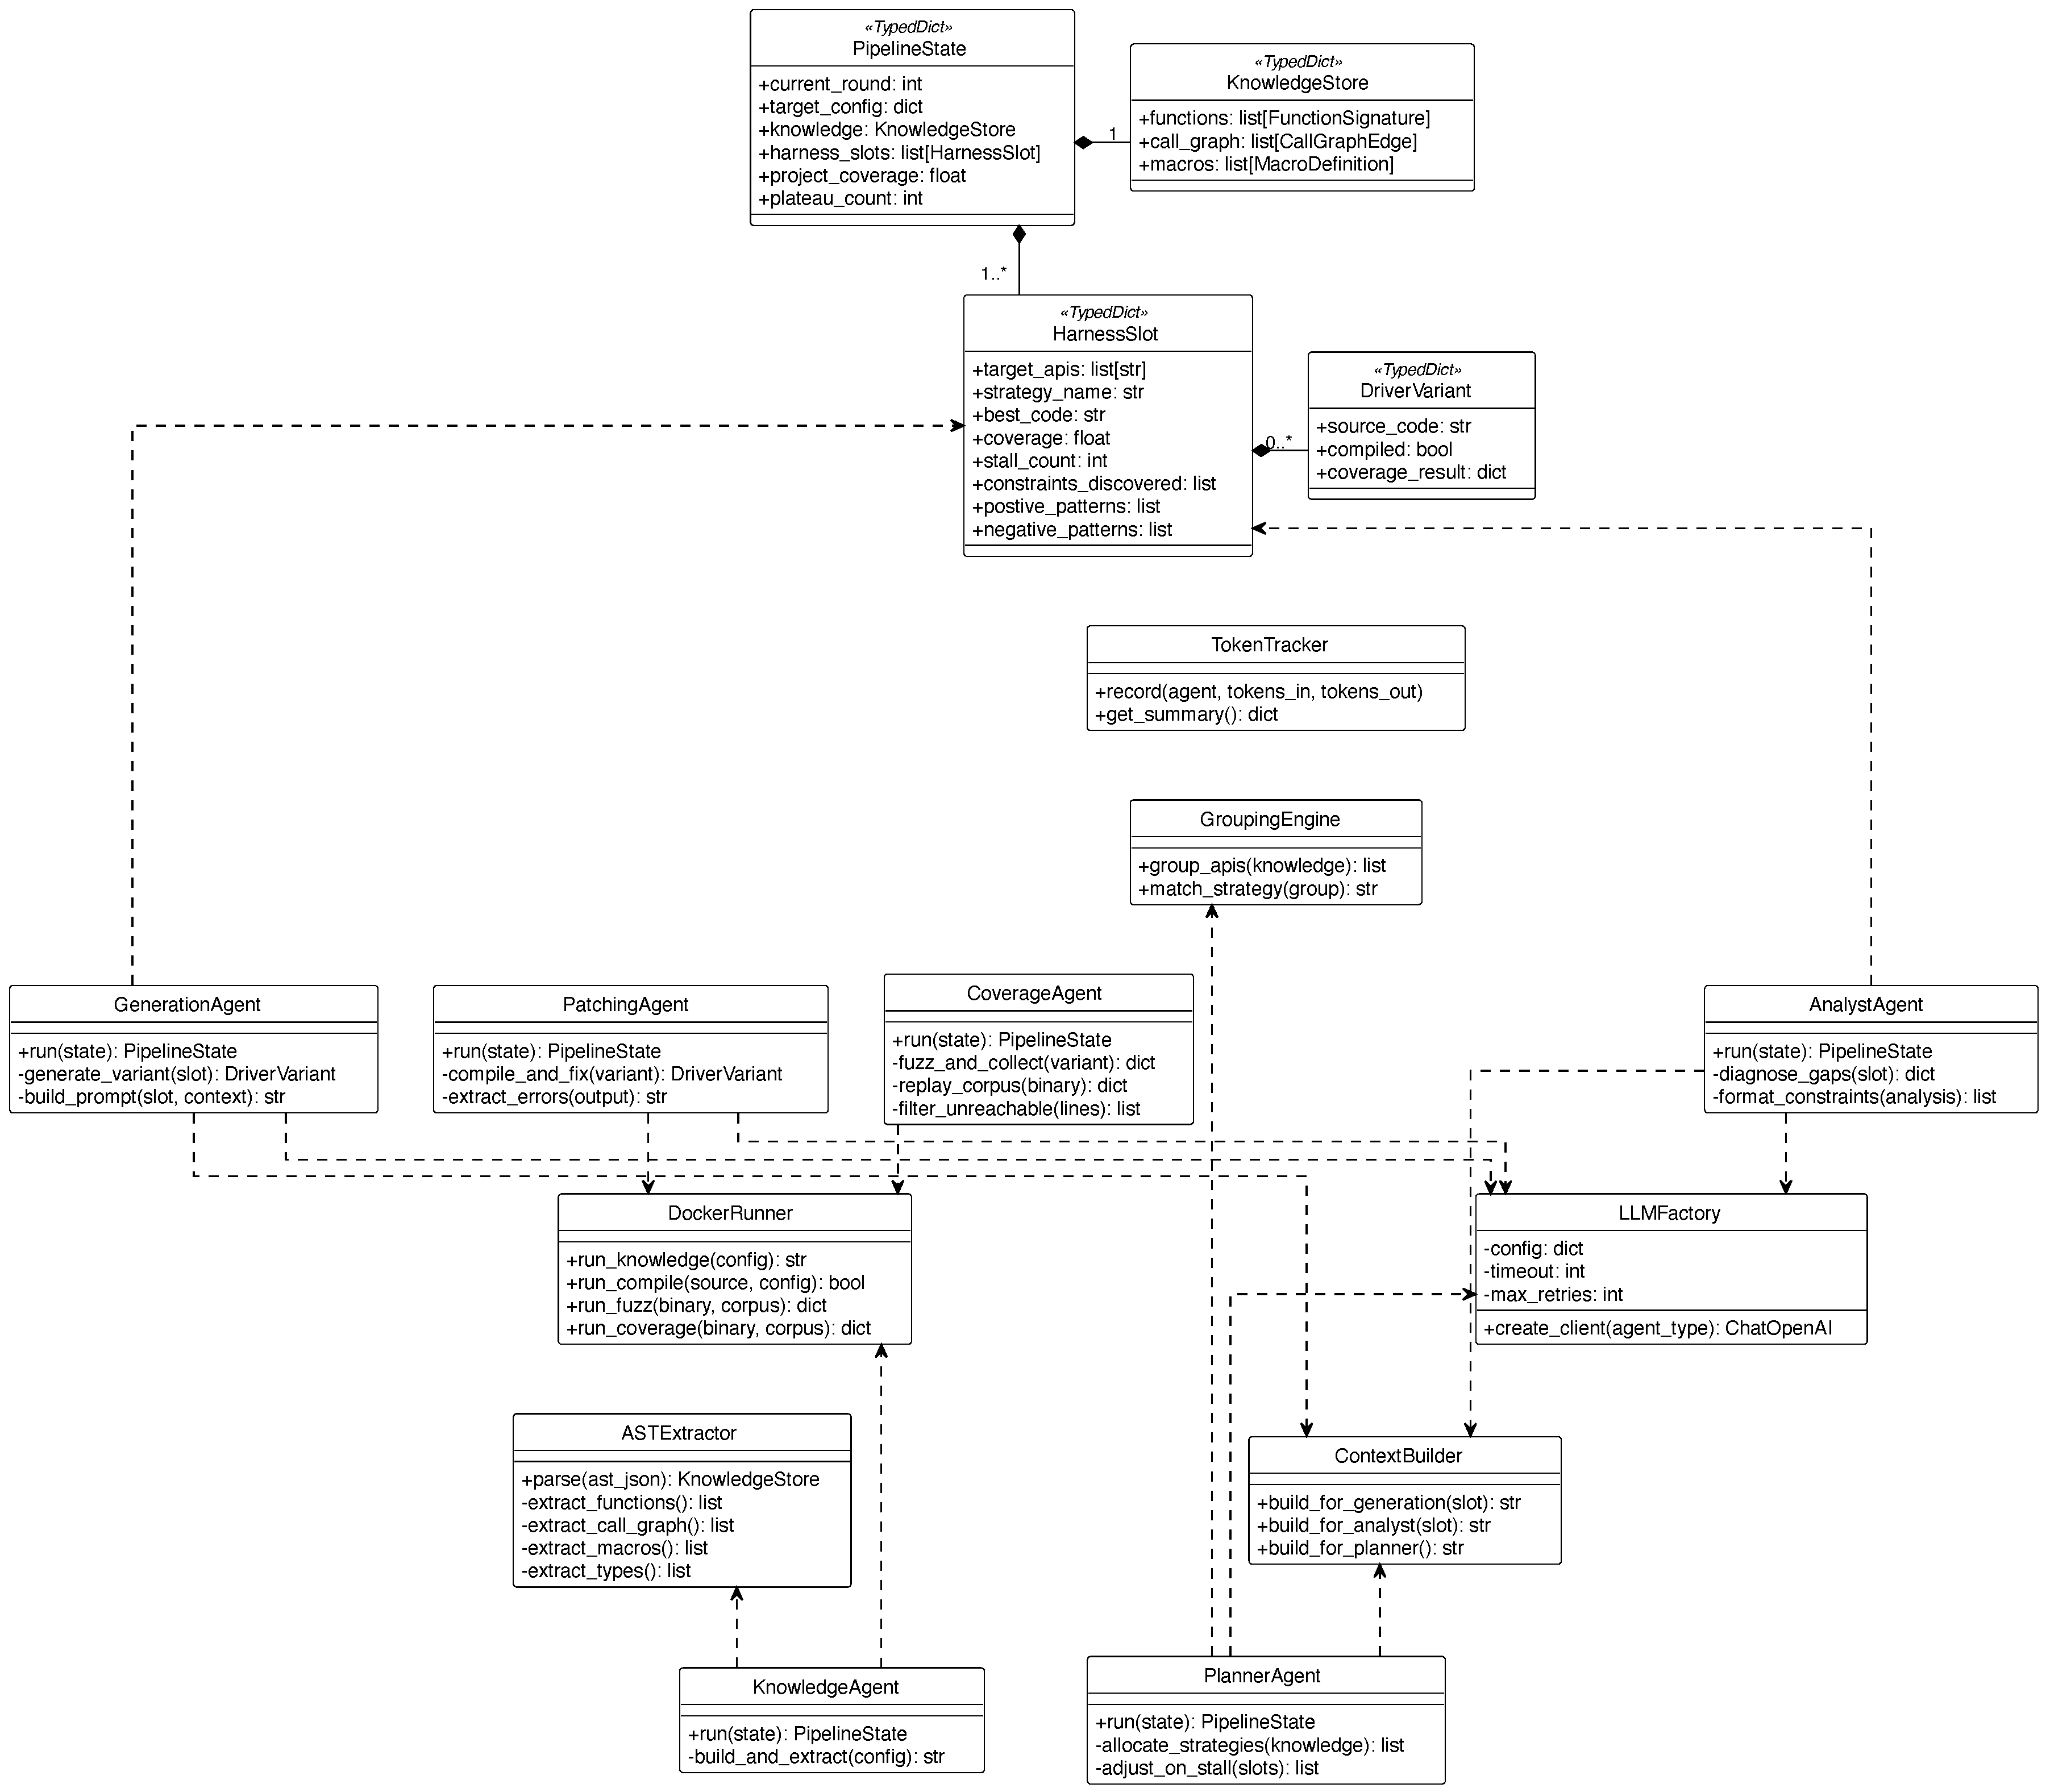
\includegraphics[width=1.2\textwidth]{images/logic_view.pdf}}
    \caption{MAGIC4FDG系统逻辑视图}
    \label{fig:logic-view}
\end{figure}

这个逻辑视图用概念类图展示系统的静态结构。在看各模块的类之前，先说明全局状态，这是理解整个系统数据流的关键。MAGIC4FDG用共享状态架构，模块之间靠一个统一的状态对象传数据。这个状态由四个类型支撑：PipelineState是最外层的容器，TypedDict定义，包含当前轮次、目标库配置、知识库、槽位列表等信息，所有模块都通过它交换信息；HarnessSlot代表一个独立的驱动槽位，里面有目标API列表、策略名、最佳代码、覆盖率、停滞计数和累积知识，这是整个系统中最核心的数据结构，因为多驱动并行迭代全靠它；DriverVariant相对简单，表示单轮生成的一个变体，包含源码、编译状态和覆盖率；KnowledgeStore存储全局知识，包括函数签名、调用图、宏定义等。

下面按3.3.2的模块划分，分别介绍各模块的核心类。

\textbf{基础设施模块}包含DockerRunner、LLMFactory和TokenTracker三个类。DockerRunner封装四类Docker操作（知识提取、编译、模糊测试、覆盖率收集），每类对应一个方法，内部负责命令构建、卷挂载管理和容器输出解析。LLMFactory用工厂模式根据配置创建带重试和超时控制的ChatOpenAI客户端。TokenTracker通过回调记录每次模型调用的令牌数，按智能体类型分类统计。

\textbf{知识处理模块}包含ASTExtractor、ContextBuilder和GroupingEngine三个类。ASTExtractor解析clang导出的AST JSON，提取FunctionSignature、CallGraphEdge和MacroDefinition等结构化对象。ContextBuilder根据调用方智能体的类型把原始知识格式化为不同粒度的文本片段。GroupingEngine基于调用图连通分量做API分组，并通过规则引擎把策略元数据的适用条件与API分组特征匹配。

\textbf{知识提取模块}的核心类是KnowledgeAgent，封装了Docker容器内目标库构建和AST导出的完整流程，调用DockerRunner执行容器操作，把结果写入全局状态的KnowledgeStore。

\textbf{策略规划与代码生成模块}里有两个核心类：PlannerAgent和GenerationAgent。前者负责加载策略库元数据、让LLM分析API语义然后做策略匹配，最终给出每个槽位该用什么策略。后者拿到分配方案后组装提示词，用线程池并行调LLM，一次生成多个变体。

\textbf{编译修复模块}的核心类是PatchingAgent。逻辑较为清晰，在Docker里编译，通过则标记成功，未通过则将错误信息提供给LLM修复，最多三次机会。

\textbf{模糊测试与覆盖率收集模块}的CoverageAgent较为复杂，它将模糊测试执行、语料库重放、覆盖率导出和CFG可达性分析串联在一起，同样通过线程池并行处理多个变体。

\textbf{缺口诊断模块}的AnalystAgent读各槽位的覆盖率数据和未覆盖行列表，调LLM做根因分析，输出约束和未覆盖代码簇，然后追加到对应槽位的知识空间里。

\subsection{系统开发视图}

开发视图关注代码的模块化结构和组织方式，描述代码如何被分解为模块、组件和包。图\ref{fig:dev-view}是MAGIC4FDG的开发视图。

\begin{figure}[H]
    \centering
    \makebox[\textwidth]{{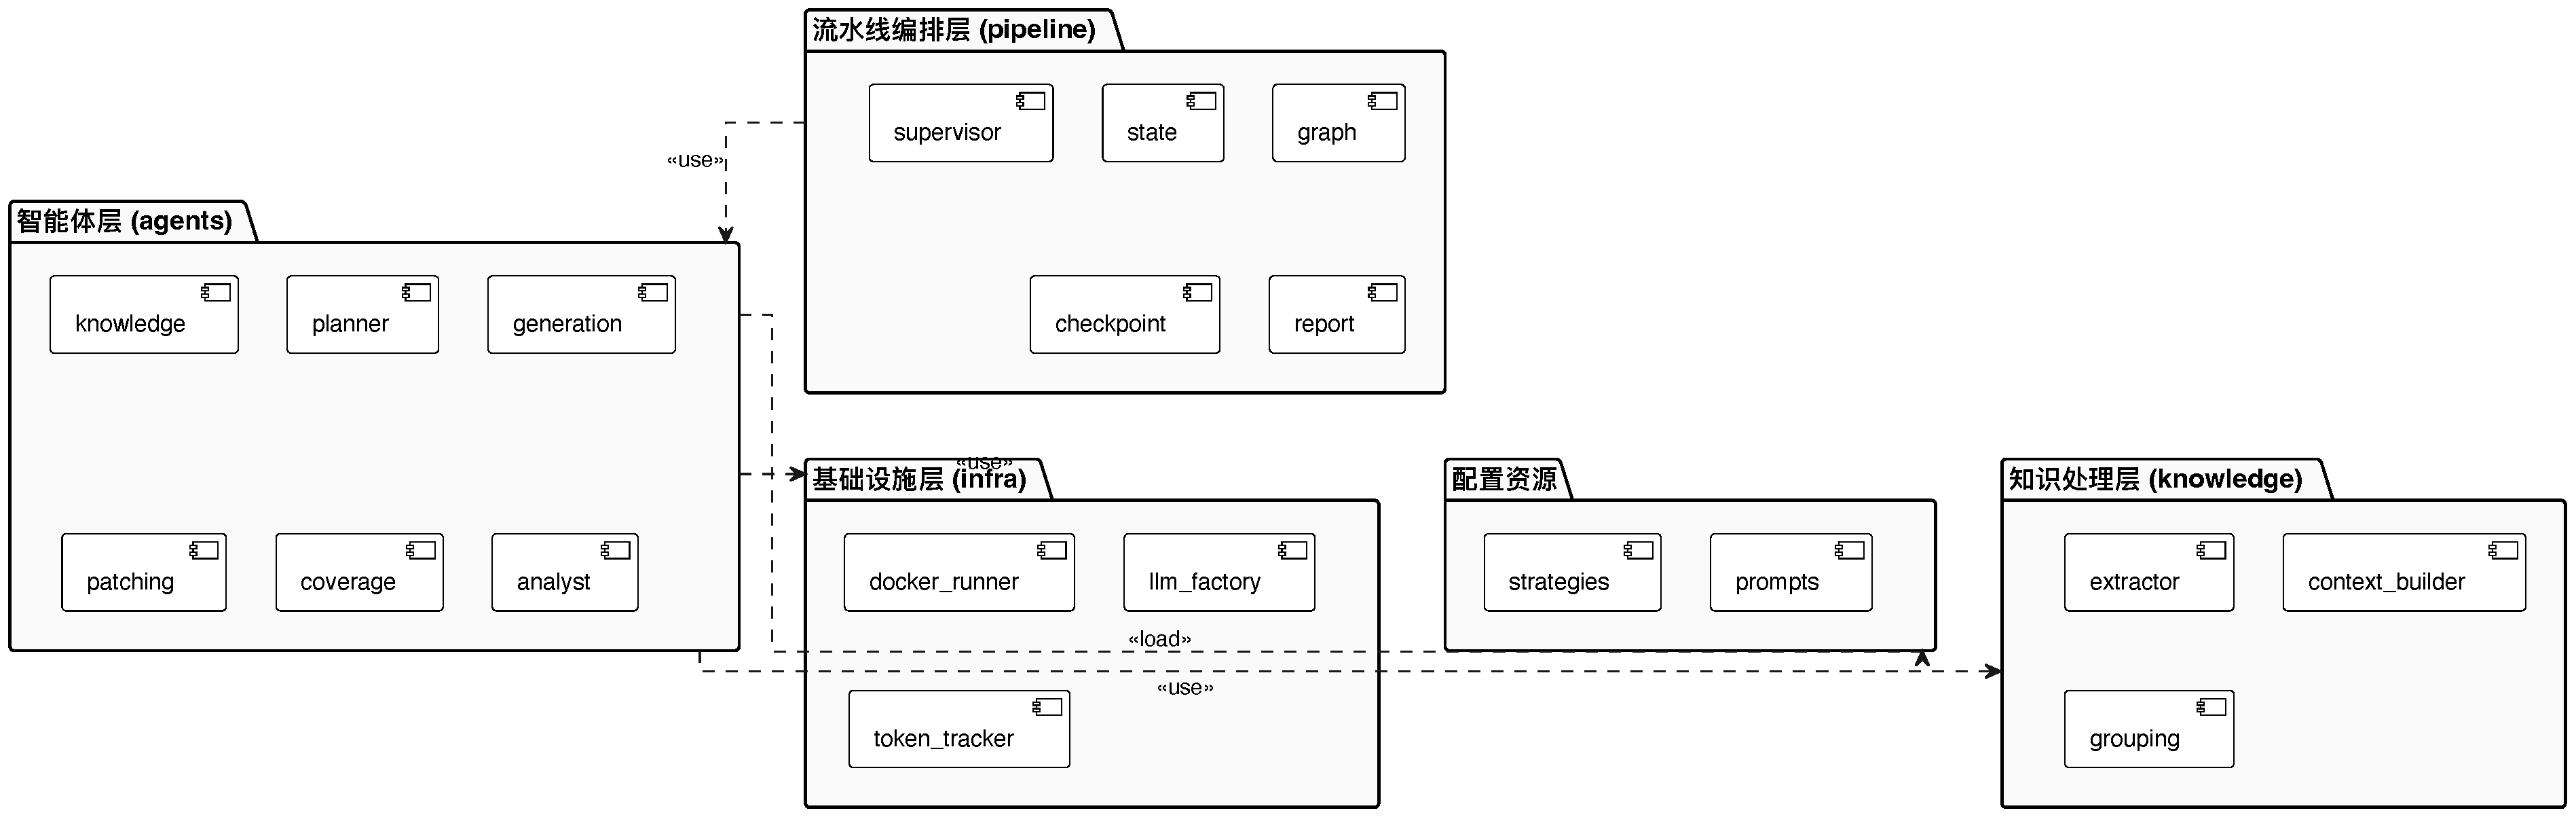
\includegraphics[width=1.2\textwidth]{images/development_view.pdf}}}
    \caption{MAGIC4FDG系统开发视图}
    \label{fig:dev-view}
\end{figure}

这个开发视图用包图展示了代码组织结构，面向开发人员设计。它遵循分层原则，自底向上分为四个代码层次：基础设施层、知识处理层、智能体层和流水线编排层。需要说明的是，代码层次划分是从软件工程的代码组织角度出发的，与3.3.2中按业务功能划分的七个模块存在映射关系：基础设施层对应基础设施模块，知识处理层对应知识处理模块，智能体层包含知识提取、策略规划与代码生成、编译修复、模糊测试与覆盖率收集、缺口诊断五个模块的实现，流水线编排层负责全局状态定义、DAG图构建、条件路由和检查点管理。

基础设施层（infra）包含docker\_runner、llm\_factory和token\_tracker三个包，分别封装Docker操作、LLM客户端创建和令牌统计。

知识处理层（knowledge）包含extractor、context\_builder和grouping三个包，分别负责AST JSON解析、按需格式化提示词文本、以及基于调用图的API分组和规则引擎策略匹配。

智能体层（agents）包含knowledge、planner、generation、patching、coverage和analyst六个包，每个包对应一个专职智能体，实现独立的节点函数，内部封装了提示词加载、LLM调用和结果解析的完整逻辑。

流水线编排层（pipeline）包含state、graph、supervisor、checkpoint和report五个包。state定义全局状态的TypedDict结构；graph构建LangGraph状态图并注册节点和条件路由；supervisor提供命令行入口和参数解析；checkpoint实现状态的JSON序列化与反序列化；report生成Markdown和JSON格式的实验报告。

另外还有两个辅助目录：strategies目录存储十种策略的Markdown文件（含YAML前置元数据），prompts目录存储各智能体的提示词模板。这两个目录作为配置资源，被智能体层在运行时动态加载。

\subsection{系统进程视图}

进程视图关注系统运行时的行为，描述并发性、进程间通信和同步机制。图\ref{fig:process-view}是MAGIC4FDG的进程视图。

\begin{figure}[H]
    \centering
    \makebox[\textwidth]{{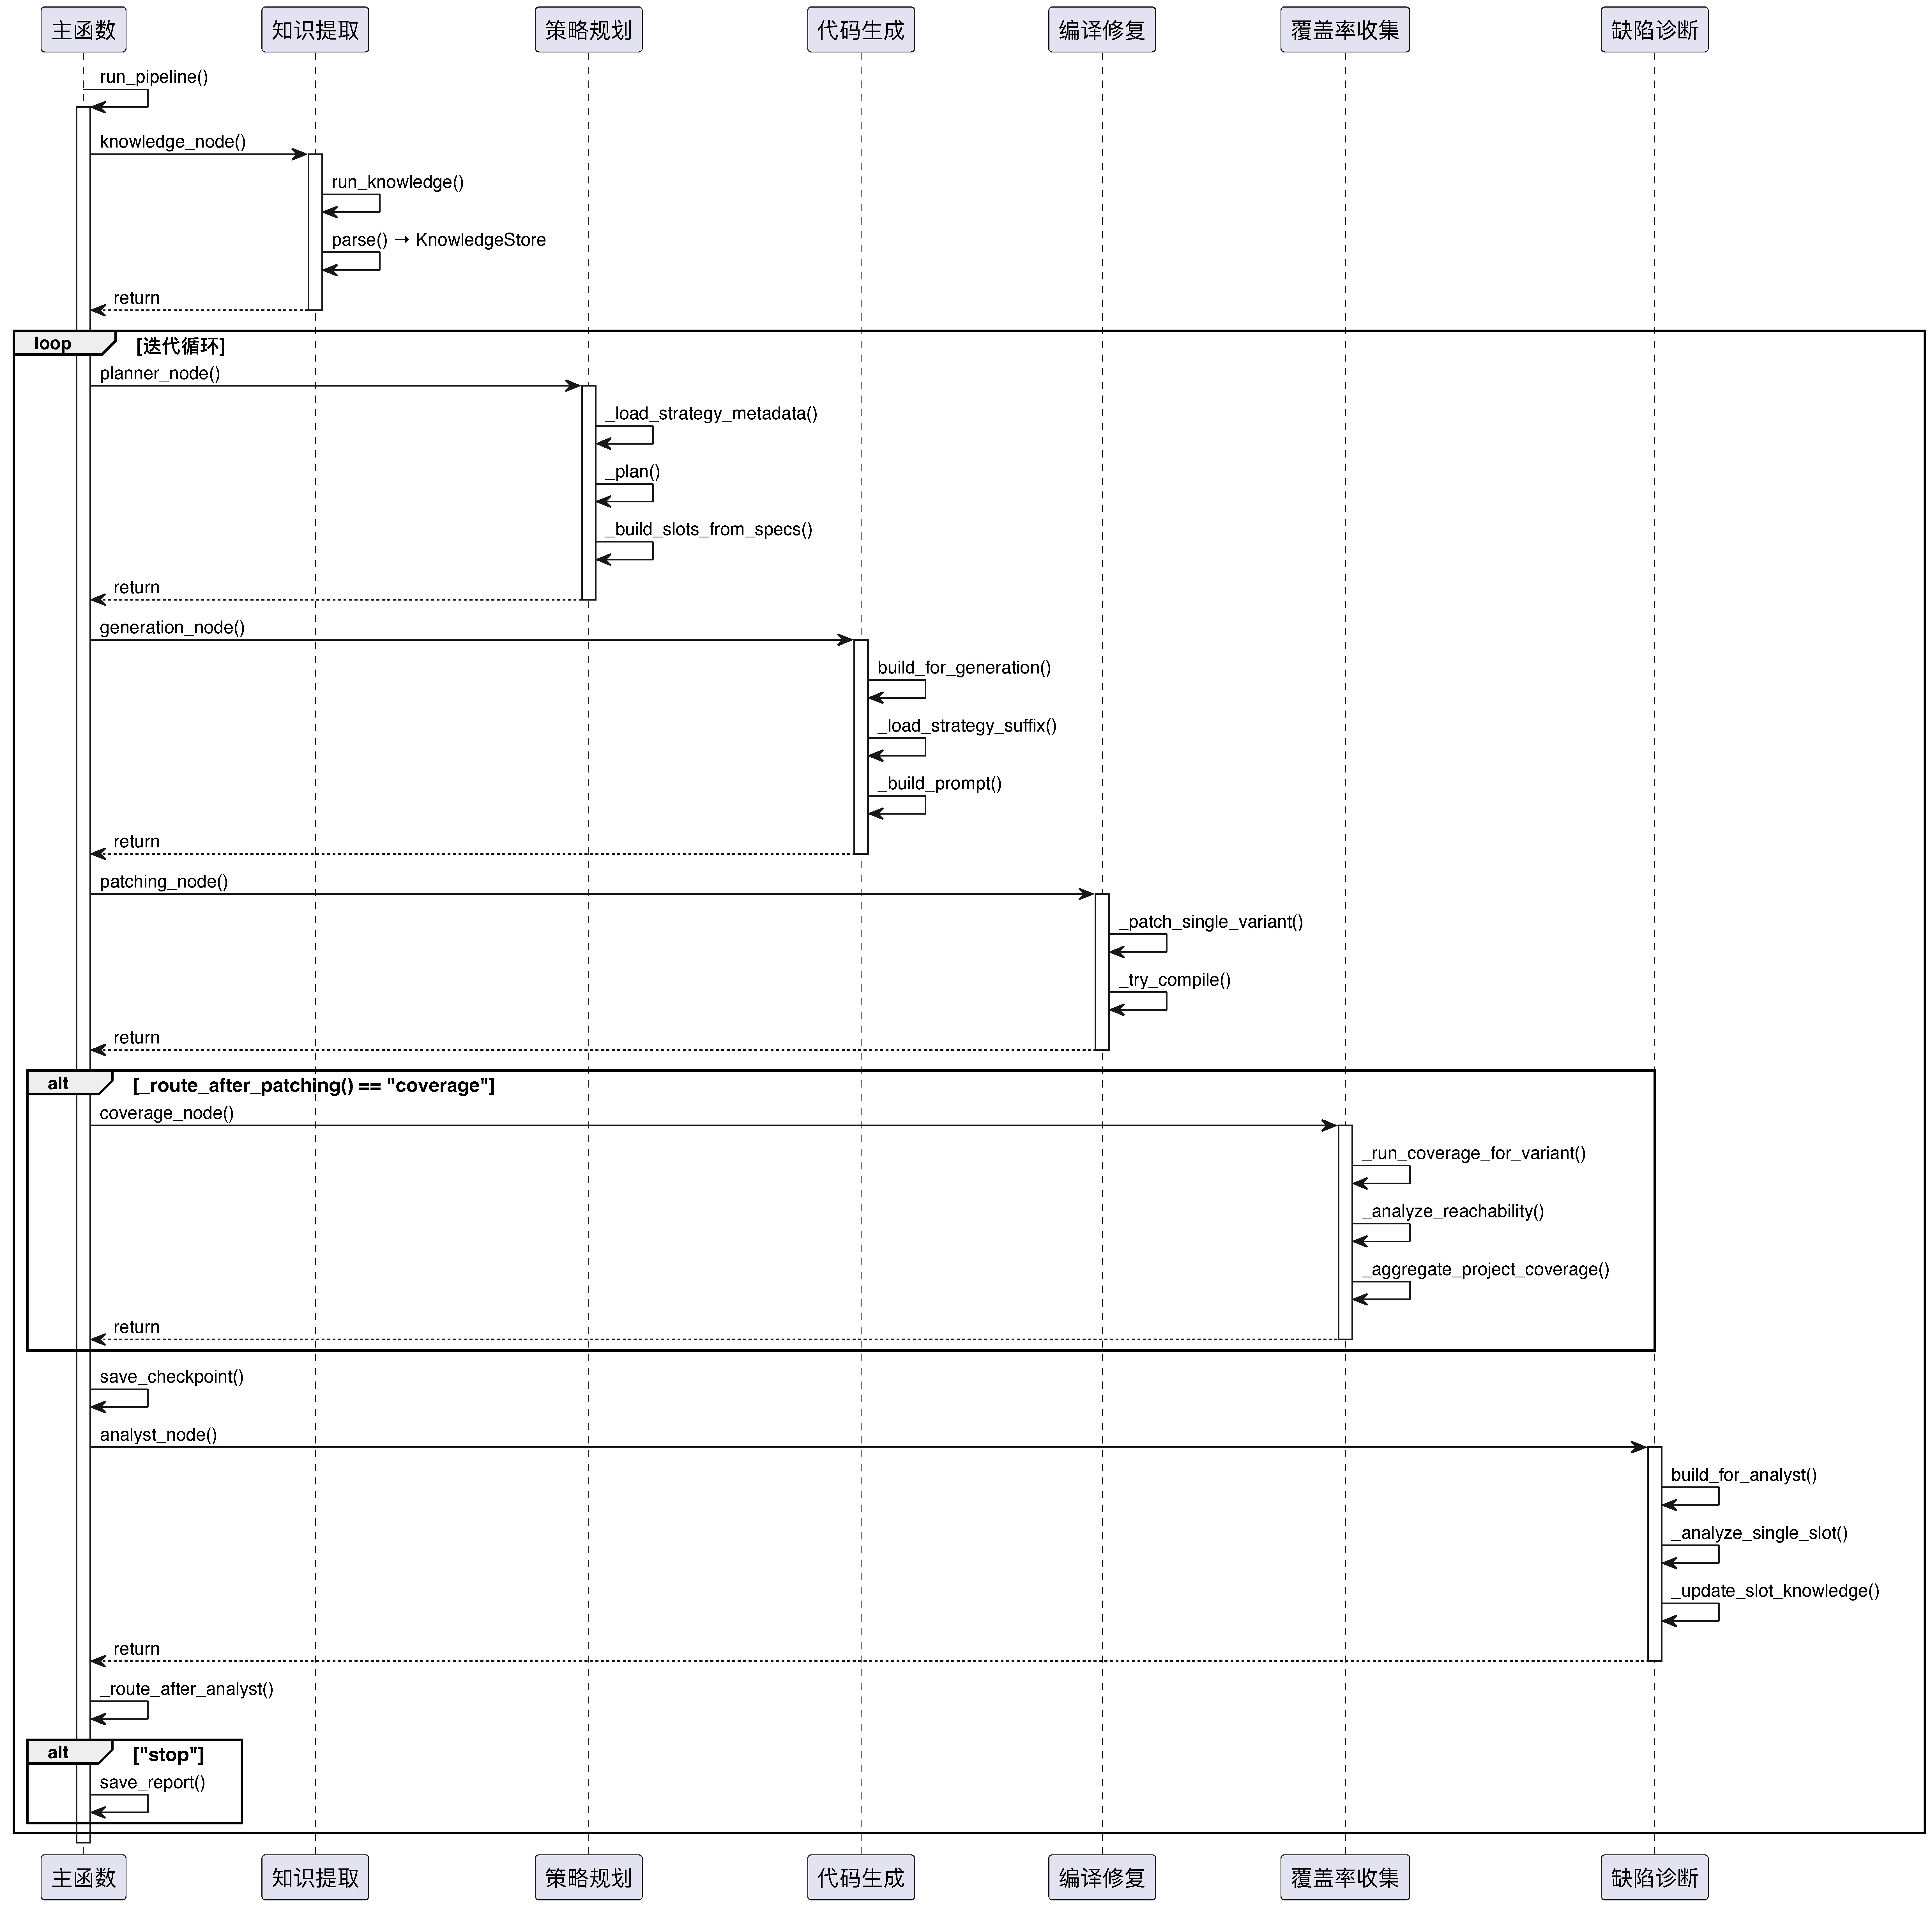
\includegraphics[width=1.1\textwidth]{images/seq_view.pdf}}}
    \caption{MAGIC4FDG系统进程视图}
    \label{fig:process-view}
\end{figure}

这个进程视图用顺序图展示系统运行时各组件的交互过程。重点展示事件触发和数据流转。系统共有八个组件在主函数的调度下协同工作：知识提取、知识处理、策略规划、代码生成、编译修复、覆盖率收集、状态持久化、缺口诊断。

主函数调用\texttt{run\_pipeline()}启动流水线后，先调用知识提取组件的\texttt{knowledge\_node()}。知识提取组件内部调用\texttt{run\_knowledge()}在Docker容器内编译目标库并做AST导出，再调用知识处理组件的\texttt{parse()}解析AST JSON，把结构化知识存入KnowledgeStore，构建产物缓存到宿主机。这一步只在首次运行时执行，后续通过检查缓存是否存在来决定是否跳过。

知识提取完成后进入迭代循环。每轮迭代中，主函数先调用策略规划组件的\texttt{planner\_node()}。该组件依次调用\texttt{\_load\_strategy\_metadata()}加载策略库元数据，首轮调用\texttt{\_plan\_initial()}通过LLM做API语义分析和策略匹配，后续轮次调用\texttt{\_plan\_iterate()}根据停滞计数调整策略，最后调用\texttt{\_build\_slots\_from\_specs()}构建槽位。

然后主函数调用代码生成组件的\texttt{generation\_node()}。该组件先调用知识处理组件的\texttt{build\_for\_generation()}获取格式化的API知识上下文，再调用\texttt{\_load\_strategy\_suffix()}加载策略后缀，最后根据轮次调用\texttt{\_build\_fresh\_prompt()}或\texttt{\_build\_incremental\_prompt()}组装提示词并调用LLM生成代码。

接着主函数调用编译修复组件的\texttt{patching\_node()}。该组件通过线程池对每个变体并行调用\texttt{\_patch\_single\_variant()}，内部调用\texttt{\_try\_compile()}在Docker容器内编译，失败的提取错误让LLM修复，最多三次。

编译修复完成后，主函数调用\texttt{\_route\_after\_patching()}做条件路由。有编译通过的变体就调用覆盖率收集组件的\texttt{coverage\_node()}，该组件通过线程池并行调用\texttt{\_run\_coverage\_for\_variant()}执行模糊测试和覆盖率收集，再调用\texttt{\_analyze\_reachability()}做CFG可达性分析，最后调用\texttt{\_aggregate\_project\_coverage()}算项目级覆盖率。全部编译失败则跳过直接进入下一步。

之后主函数调用状态持久化组件的\texttt{checkpoint\_node()}，内部调用\texttt{save\_checkpoint()}把流水线状态序列化为JSON检查点文件，同时保存各变体源码。

最后主函数调用缺口诊断组件的\texttt{analyst\_node()}。该组件先调用知识处理组件的\texttt{build\_for\_analyst()}获取未覆盖代码行的上下文，再通过线程池对每个活跃槽位并行调用\texttt{\_analyze\_single\_slot()}做根因分析，最后调用\texttt{\_update\_slot\_knowledge()}把结果追加到对应槽位的知识空间。

每轮迭代结束时，主函数调用\texttt{\_route\_after\_analyst()}检查终止条件（覆盖率达标、轮次上限、全部收敛、项目级停滞）。满足任一条件就调用\texttt{save\_report()}生成报告并终止；否则进入下一轮。

\subsection{系统物理视图}

物理视图关注部署架构，描述软件如何映射到硬件资源。图\ref{fig:deploy-view}是MAGIC4FDG的物理视图。

\begin{figure}[htbp]
    \centering
    \makebox[\textwidth]{{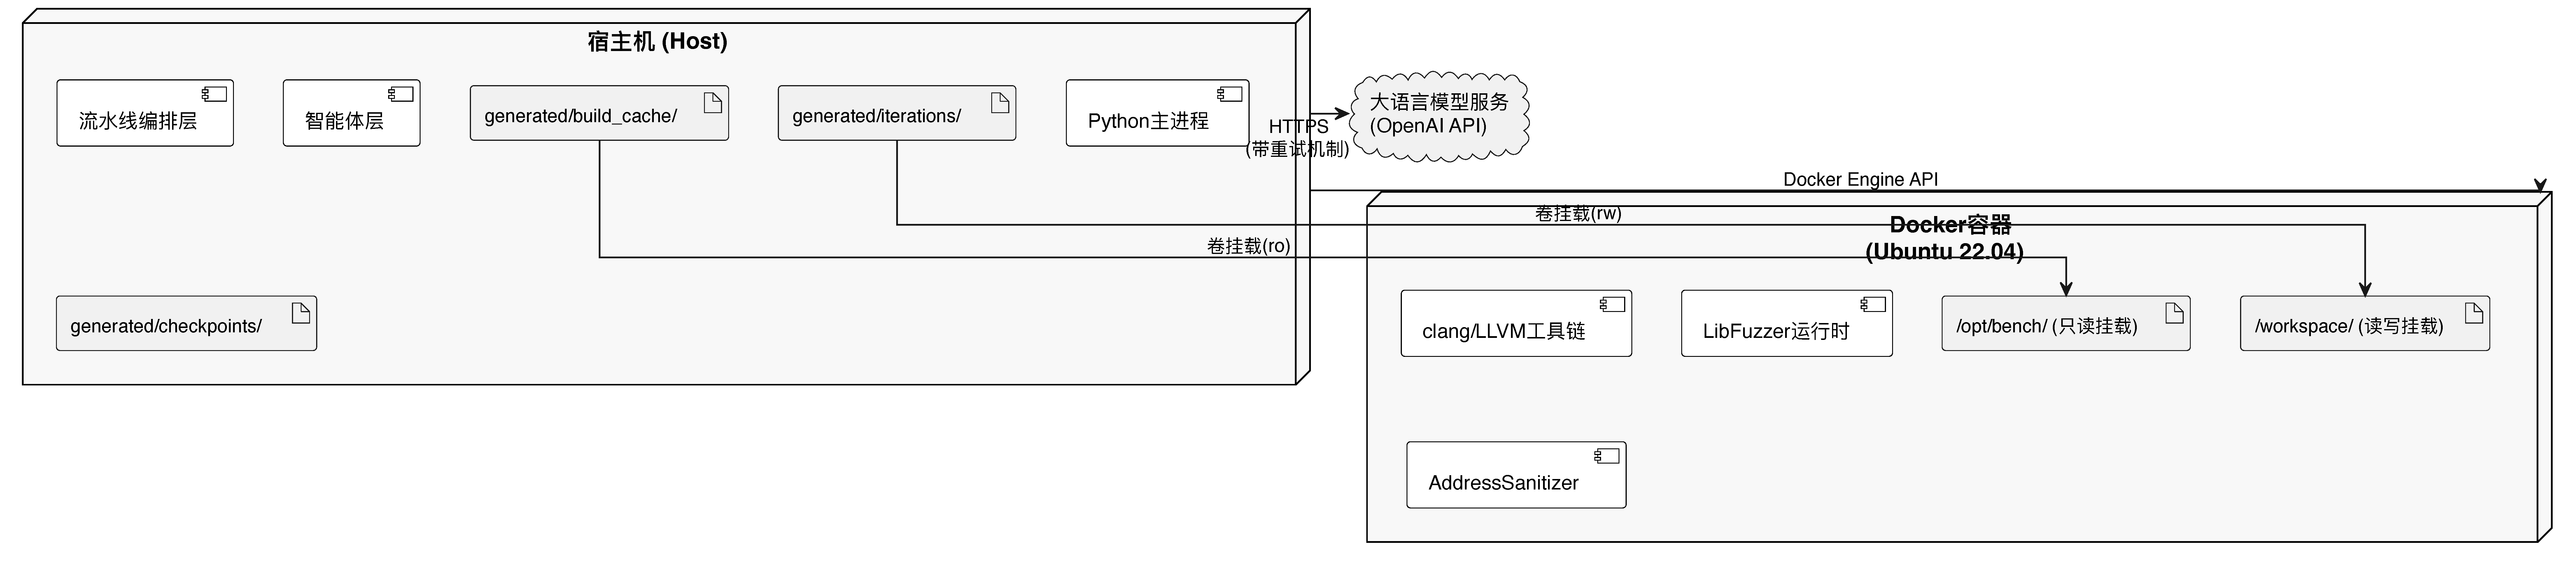
\includegraphics[width=\textwidth]{images/phy_view.drawio.pdf}}}
    \caption{MAGIC4FDG系统物理视图}
    \label{fig:deploy-view}
\end{figure}

部署结构分三块看：宿主机、Docker容器、LLM服务。

宿主机运行的是Python主进程，负责流水线编排和智能体调度。计算密集型操作（构建目标库、编译驱动、执行模糊测试、收集覆盖率）全部在Docker容器内完成。这一设计基于实际考虑——macOS上clang的行为与Linux不完全一致，直接在宿主机编译容易出现链接兼容性问题，因此统一使用Ubuntu 22.04容器，预装好clang/LLVM工具链和LibFuzzer。宿主机与容器之间通过卷挂载交换数据，构建缓存挂载为只读（/opt/bench），驱动源码和语料库通过读写卷双向传递。

LLM服务通过HTTPS调用，策略规划、代码生成、编译修复、缺口诊断四个环节都需要使用。本系统使用兼容OpenAI API格式的端点，配置文件中指定地址和密钥。考虑到网络波动，系统采用指数退避重试机制，实测中偶有超时但不会导致流水线中断。

\section{本章小结}

这一章完成了需求分析和概要设计，为后续的详细设计和编码实现提供了依据。

回顾一下本章内容。开头用流程图将系统运行的四个阶段阐述清楚，即知识准备、驱动生成与编译修复、模糊测试与覆盖率收集、缺口诊断与迭代控制，每个阶段中哪些智能体参与、如何配合都做了说明。

需求分析部分，本章梳理了三类涉众各自关心什么，再从中提炼出8项功能性需求和9项非功能性需求。用例分析画了用例图，选取了10个关键用例做了详细描述。用例描述较为详细，目的是为后续实现提供明确的验收标准。

概要设计部分，本章将系统划分为七个功能模块，分析了它们之间的数据依赖、功能依赖和状态依赖。然后用"4+1"视图从不同角度描述架构：逻辑视图描述类和依赖关系，开发视图描述代码组织与分层，进程视图描述运行时调用顺序和并行点，物理视图描述部署结构及三者间的通信方式。场景视图即前述用例图，此处不再赘述。
\chapter{MAGIC4FDG系统的详细设计与实现}

第三章完成了需求分析和概要设计，本章在此基础上对核心模块进行详细设计和实现展示。本章将逐一剖析知识提取模块、策略规划与代码生成模块、模糊测试与覆盖率收集模块、缺口诊断模块的内部结构和实现机制。每节先用类图和顺序图说明设计思路，再结合关键代码片段展示核心功能的具体实现。

\section{知识提取模块详细设计与实现}

知识提取模块是整个系统的基础，没有它提供的结构化API知识，后面的智能体就无从下手。它的职责是在Docker容器内编译目标库并做clang AST导出，从中提取结构化的API知识，再根据不同智能体的需求把知识格式化为适合注入提示词的文本片段。下面先通过类图和顺序图说明设计思路，再深入解析AST解析与知识构建、差异化上下文构建两个核心功能的实现。

\subsection{知识提取模块详细设计}

图\ref{fig:knowledge-class}是知识提取模块的详细设计类图，展示了关键类及其属性和方法。


模块入口为\texttt{extract\_knowledge}函数，接收目标库配置后依次执行AST解析、宏提取、调用图构建、语义标注、注释附加五个阶段，最终产出\texttt{KnowledgeStore}对象。\texttt{KnowledgeStore}在设计上充当全局知识容器，内含四个字段。其中\texttt{api\_entries}存放全部公开API条目，每条对应一个\texttt{APIEntry}实例，记录函数名、签名、返回类型、参数列表等基本信息，同时包含功能类别、前置条件和文档注释。\texttt{call\_graph}用邻接表存储函数间的调用关系。其余两个字段分别管理类型定义（结构体、枚举、类型别名）和宏常量，宏常量还按标志位、普通常量、函数式宏做了分类，方便后续生成智能体按需取用。

\begin{figure}[H]
    \centering
    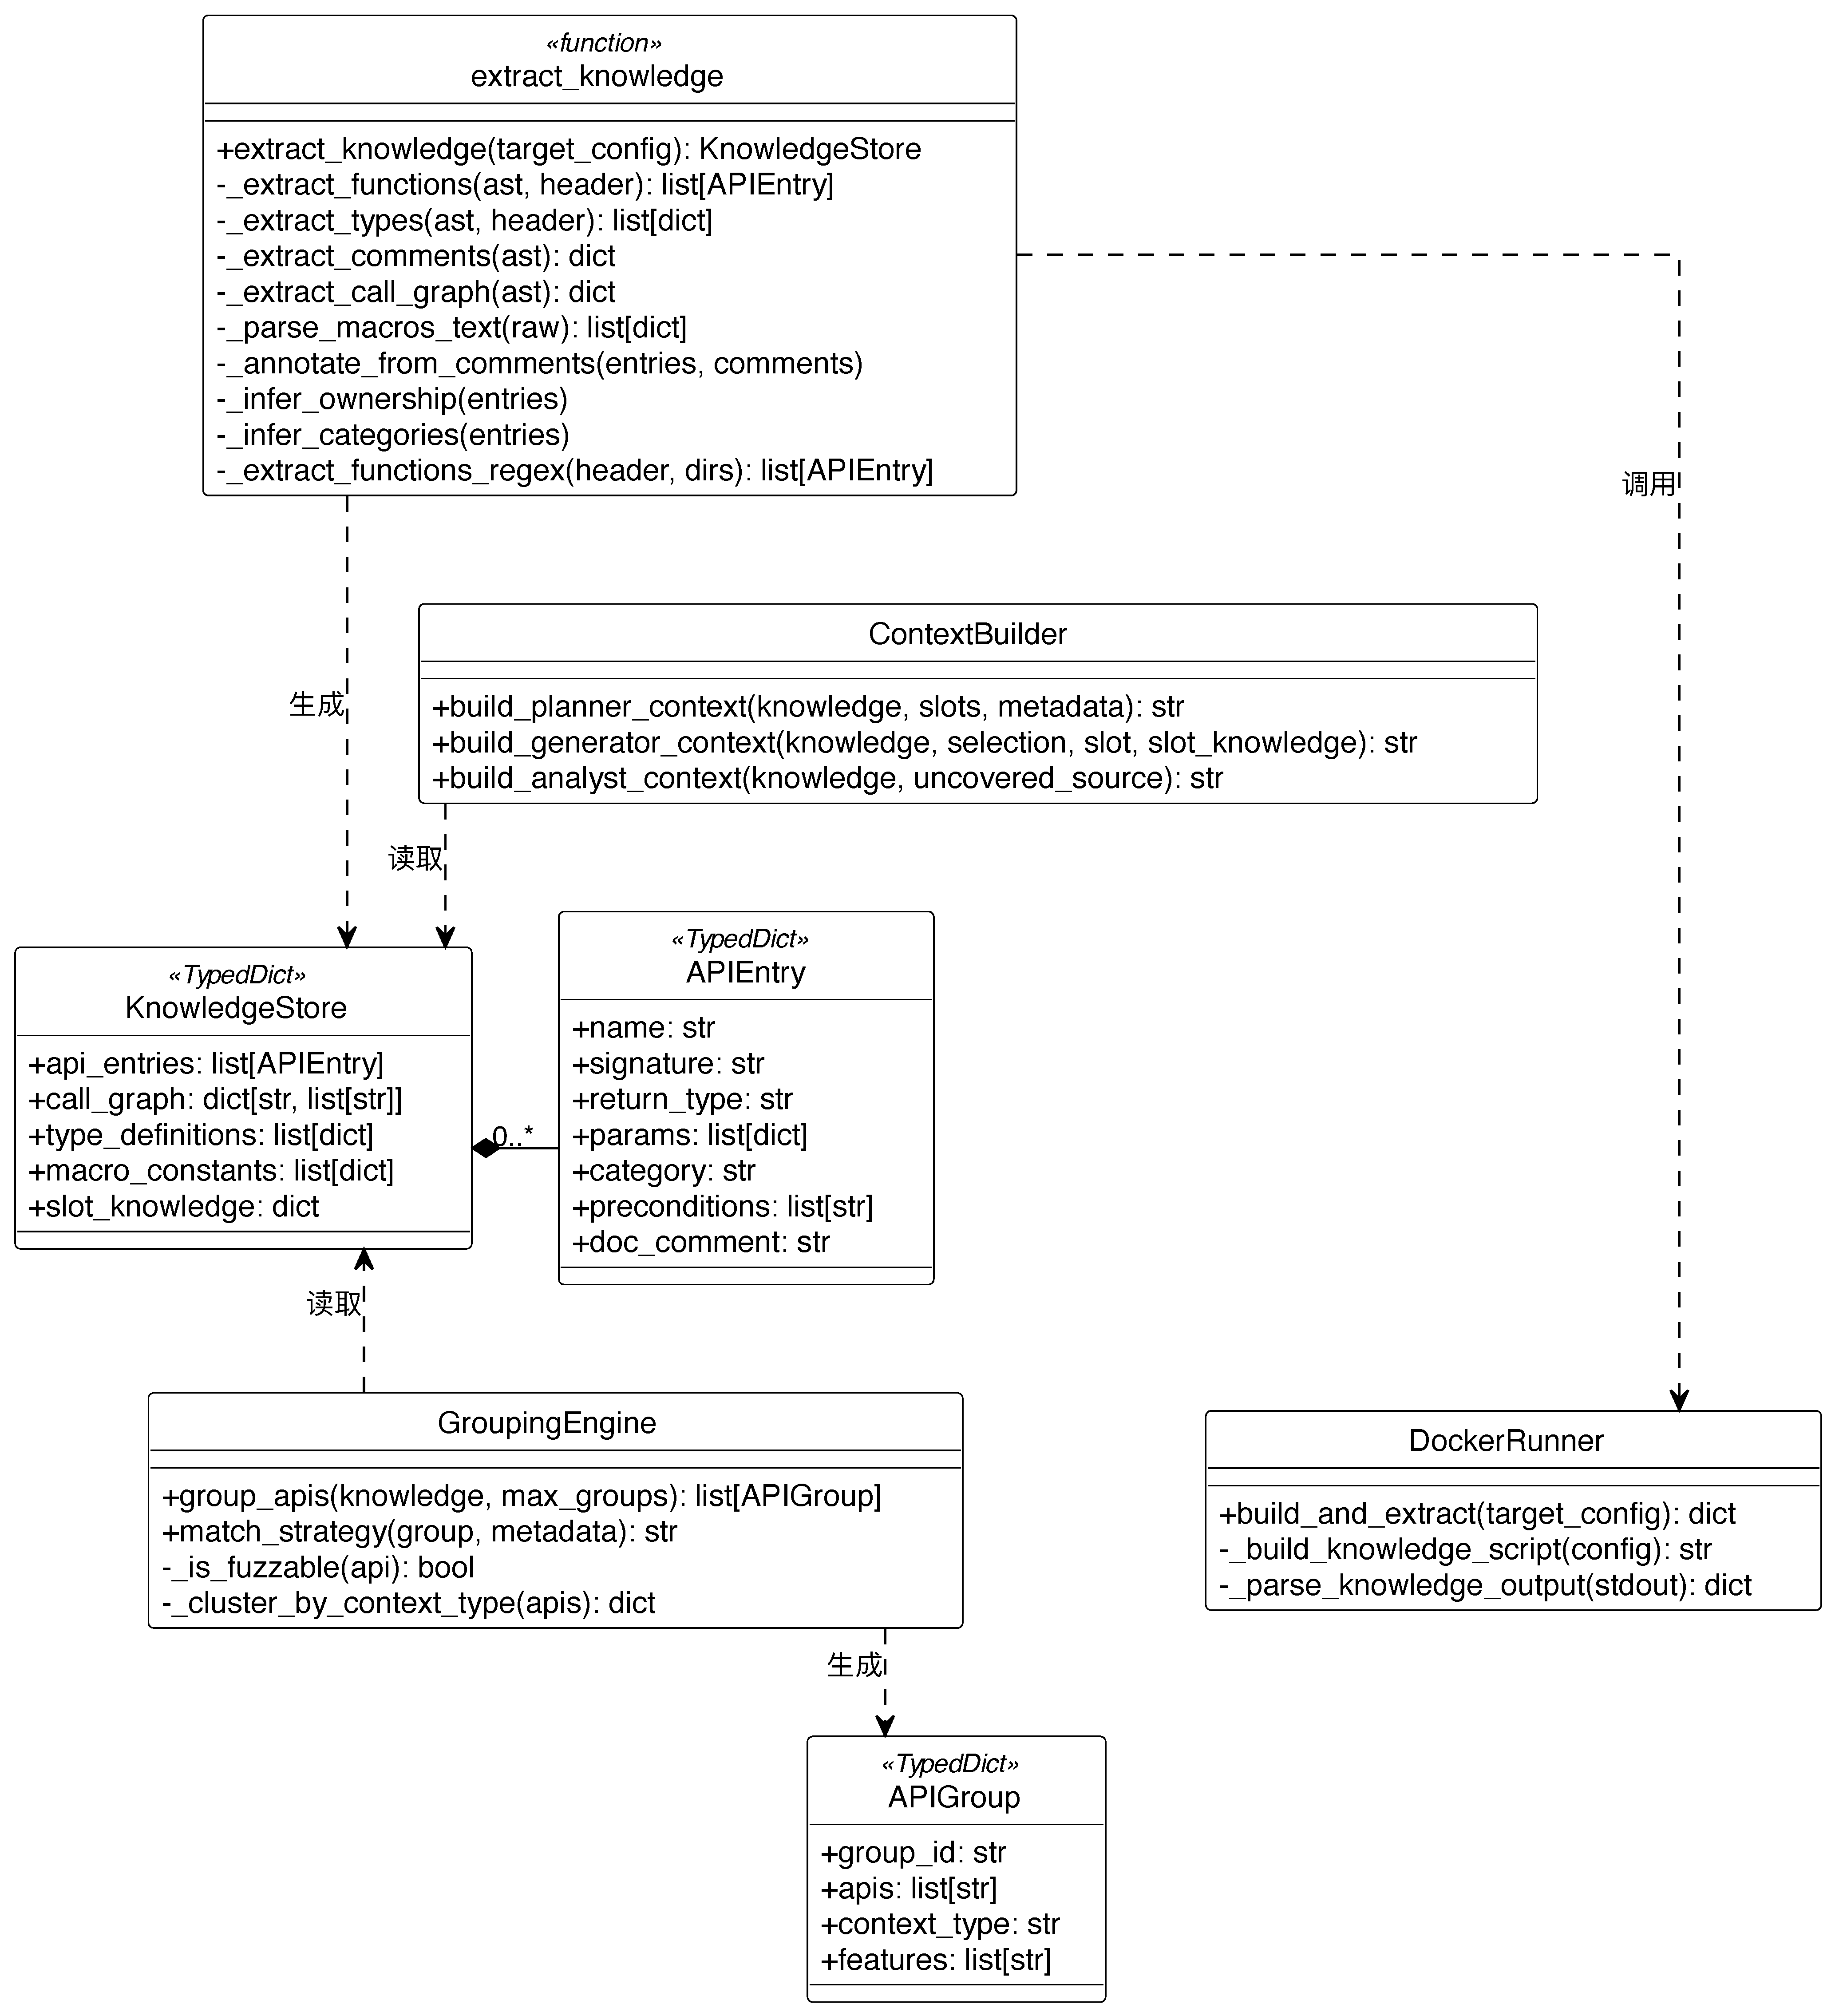
\includegraphics[width=\textwidth]{images/knowledge_class.pdf}
    \caption{知识提取模块详细设计类图}
    \label{fig:knowledge-class}
\end{figure}

\texttt{ContextBuilder}类是知识处理的核心组件，负责把原始\texttt{KnowledgeStore}转换为适合注入提示词的文本片段。它提供三个方法：\texttt{build\_planner\_context}为Planner生成API分类概览和调用图摘要；\texttt{build\_generator\_context}为Generation生成目标API完整签名、参数语义和类型定义的详细上下文；\texttt{build\_analyst\_context}为Analyst生成完整API清单和未覆盖源码行的诊断上下文。三种上下文的信息粒度和侧重点各不相同，这就是差异化上下文注入的体现。

\texttt{GroupingEngine}类实现确定性的API分组和策略匹配，作为LLM策略规划失败时的回退方案。\texttt{group\_apis}方法基于调用图连通分量和参数类型相似性做API聚类，\texttt{match\_strategy}方法用规则引擎把分组特征与策略元数据的适用条件匹配。

\begin{figure}[H]
    \centering
    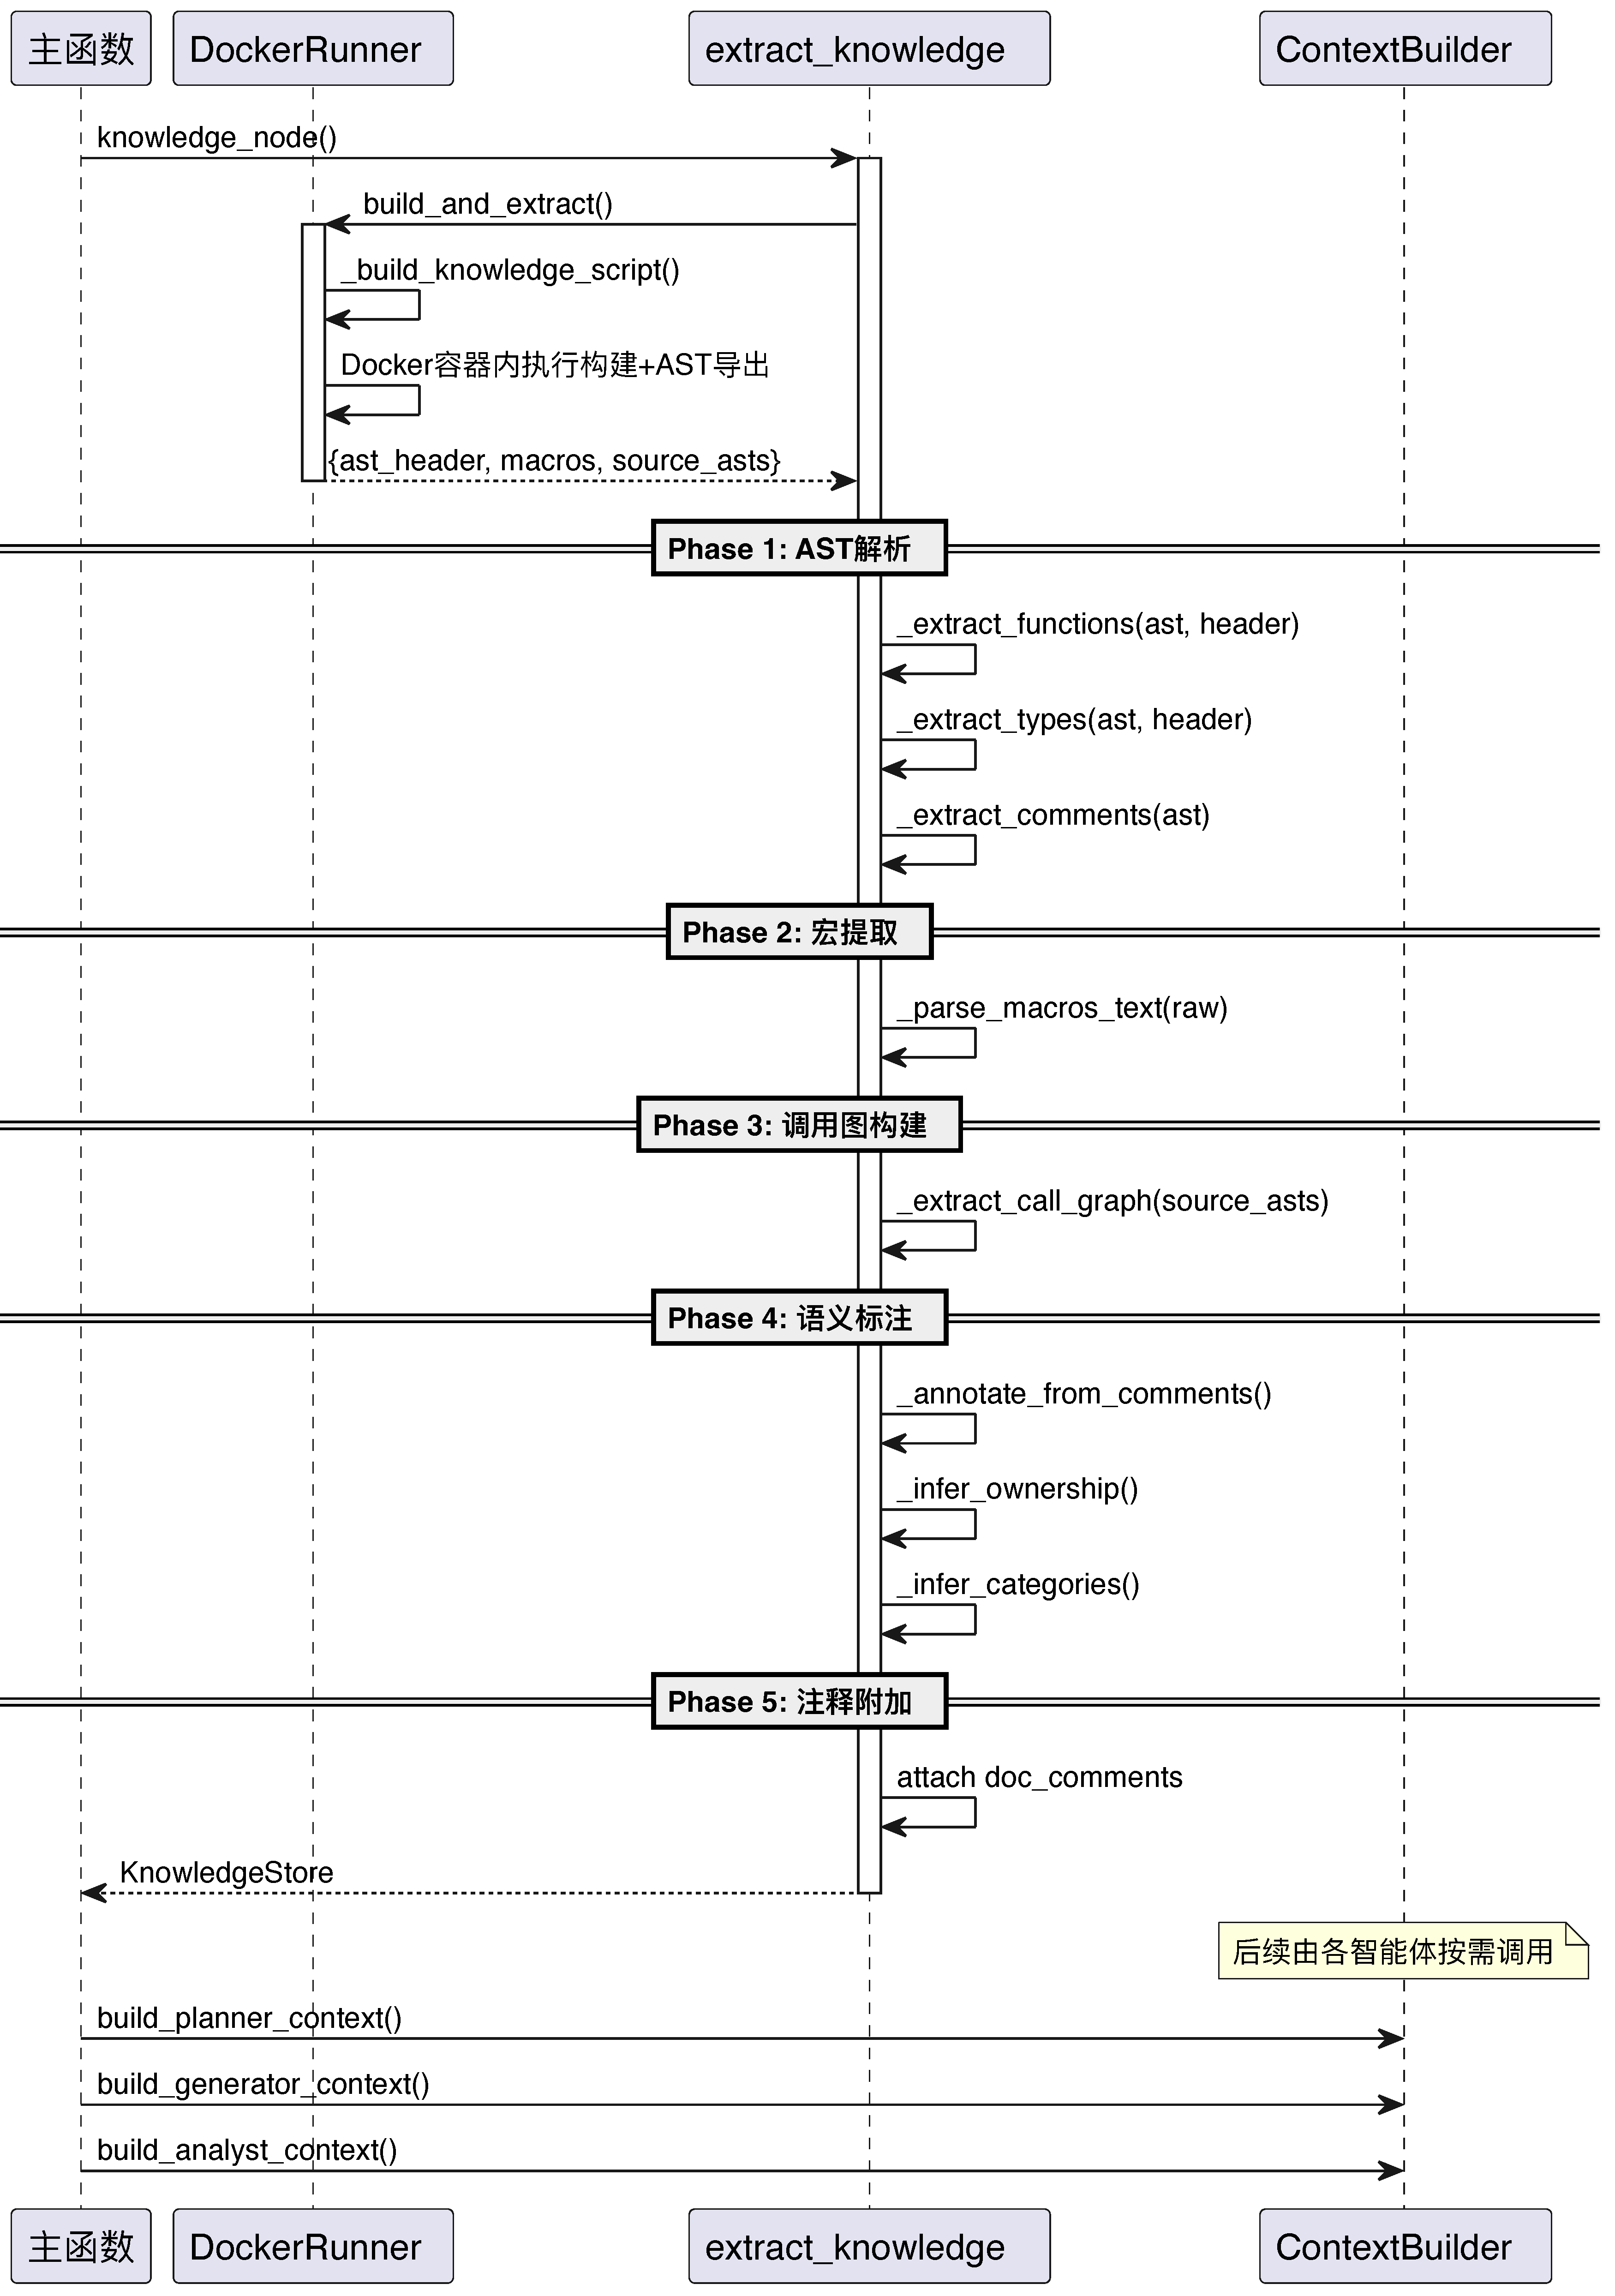
\includegraphics[width=\textwidth]{images/knowledge_seq.pdf}
    \caption{知识提取模块详细设计顺序图}
    \label{fig:knowledge-seq}
\end{figure}

图\ref{fig:knowledge-seq}是知识提取模块的顺序图，描绘了各功能类之间的协作时序。

流程从主函数调用\texttt{knowledge\_node}开始。该函数读取流水线状态中的目标库配置，随即委托\texttt{extract\_knowledge}完成实际工作。后者首先通过\texttt{DockerRunner}的\texttt{build\_and\_extract}方法，在Docker容器内完成四项操作：目标库编译、头文件AST导出、预处理器宏导出、源文件AST导出。容器执行结果经标准输出的分隔符协议传回宿主机。

获取原始数据后进入五阶段处理流水线：第一阶段调用\texttt{\_extract\_functions}解析头文件AST JSON，遍历\texttt{FunctionDecl}节点提取公开API签名；第二阶段调用\texttt{\_parse\_macros\_text}解析预处理器输出，提取并分类宏常量；第三阶段对每个源文件AST调用\texttt{\_extract\_call\_graph}，该步骤的核心逻辑在于递归查找\texttt{CallExpr}节点、将调用关系填入邻接表。第四阶段较为复杂，需要连续执行三个语义标注方法：\texttt{\_annotate\_from\_comments}、\texttt{\_infer\_ownership}、\texttt{\_infer\_categories}，从注释和命名规则中推断所有权语义、前置条件和功能类别。第五阶段将文档注释附加到对应API条目。如果AST解析阶段未能提取到任何函数声明，系统自动回退到基于正则表达式的头文件扫描方案，保证知识提取不会完全失败。


\subsection{AST解析与知识构建功能实现}

这一小节聚焦知识提取模块中AST解析与知识构建的实现细节。本节依次说明clang AST深度优先遍历算法、函数签名提取、调用图构建和语义标注这四个功能的具体做法。

\subsubsection{AST深度优先遍历}

clang以JSON格式导出的抽象语法树本质上是一棵嵌套树，每个节点通过\texttt{inner}字段持有子节点列表。本模块实现了一个通用的深度优先遍历生成器\texttt{\_walk\_ast}，它是后续所有AST分析功能的基础。这里有一个实现细节：生成器采用Python的\texttt{yield from}语法做惰性遍历，不会一次性把整棵AST展开到内存里。对于大型库（如OpenSSL，AST JSON可达数百MB），这一点至关重要。该遍历器的实现如图\ref{fig:walk-ast}所示。

\begin{figure}[H]
    \centering
    \begin{lstlisting}[style=style@python]
   def _walk_ast(node: dict):
       if not node:
           return
       yield node
       for child in node.get("inner", []):
           if child:
               yield from _walk_ast(child)
    \end{lstlisting}
    \caption{AST深度优先遍历生成器}
    \label{fig:walk-ast}
\end{figure}

\subsubsection{函数签名提取}

函数签名提取是知识构建中最关键的一步，目标在于从AST中定位所有公开API的函数声明，并提取函数名、完整类型签名、返回类型及参数列表。核心实现如图\ref{fig:extract-functions}所示。

实现中采用了逐层收窄的过滤策略。首先，通过\texttt{kind}字段筛出\texttt{FunctionDecl}节点，排除变量声明和类型定义。接着检查\texttt{loc}字段中的文件路径，只有声明在目标头文件中的函数才予以保留，系统头文件和第三方依赖引入的声明在此被剔除。最后一道过滤针对函数名前缀：以下划线开头的内部实现函数不进入结果集。通过这三道过滤的函数声明，系统从\texttt{type.qualType}字段取出完整函数类型签名，并调用\texttt{\_extract\_params}方法遍历子节点中的\texttt{ParmVarDecl}节点，逐一提取参数名、类型、是否可空和所有权语义。

当AST解析未能提取到任何函数声明时（比如目标库使用了clang无法处理的非标准扩展），系统会自动回退到基于正则表达式的头文件扫描方案。这个回退方案用多行正则匹配C函数声明的标准模式。精度虽然不如AST解析，但能保证知识提取流程不会因为单一工具链的局限而彻底失败。

\begin{figure}[H]
    \centering
    \begin{lstlisting}[style=style@python]
   def _extract_functions(ast: dict, header_path: str) -> list[APIEntry]:
       entries: list[APIEntry] = []
       header_name = Path(header_path).name if header_path else ""
       for node in _walk_ast(ast):
           if node.get("kind") != "FunctionDecl":
               continue
           loc = node.get("loc", {})
           file_field = (loc.get("file", "") or
                         loc.get("expansionLoc", {}).get("file", ""))
           if file_field and header_name and header_name not in file_field:
               continue
           name = node.get("name", "")
           if not name or name.startswith("_"):
               continue
           qual_type = node.get("type", {}).get("qualType", "")
           params = _extract_params(node)
           return_type = _infer_return_type(qual_type)
           entries.append(APIEntry(
               name=name, signature=qual_type,
               return_type=return_type, params=params,
               category="utility", preconditions=[],
               group="", doc_comment="",
           ))
       return entries
    \end{lstlisting}
    \caption{基于AST的函数签名提取}
    \label{fig:extract-functions}
\end{figure}

\subsubsection{调用图构建}

调用图记录了函数之间的调用关系，是策略规划智能体做API分组和场景设计时的重要依据。系统通过递归遍历源文件AST中的\texttt{CallExpr}节点来构建调用图，核心实现如图\ref{fig:call-graph}所示。

算法维护一个\texttt{current\_func}状态变量，遍历过程中持续跟踪当前所处的函数作用域。遇到\texttt{FunctionDecl}节点时更新当前函数名；遇到\texttt{CallExpr}节点时通过\texttt{\_resolve\_callee}解析被调用函数的名称，把调用关系记录到邻接表中。值得说明的是，\texttt{\_resolve\_callee}方法需要处理两种常见的AST表示：直接的\texttt{DeclRefExpr}引用，以及经过\texttt{ImplicitCastExpr}隐式转换的间接引用。系统对所有源文件的调用图做合并和去重，最终生成全局的函数调用关系图。

\begin{figure}[H]
    \centering
    \begin{lstlisting}[style=style@python]
   def _extract_calls_recursive(node: dict, current_func: str,
                                graph: dict) -> None:
       kind = node.get("kind", "")
       if kind == "FunctionDecl":
           current_func = node.get("name", "")
       elif kind == "CallExpr" and current_func:
           for child in node.get("inner", []):
               callee = _resolve_callee(child)
               if callee:
                   graph.setdefault(current_func, []).append(callee)
                   break
       for child in node.get("inner", []):
           if child:
               _extract_calls_recursive(child, current_func, graph)
    \end{lstlisting}
    \caption{调用图递归构建}
    \label{fig:call-graph}
\end{figure}

\subsubsection{语义标注}

语义标注阶段要解决的问题是，光有函数签名还不够，代码生成智能体需要知道如何正确调用这些API。因此本模块从文档注释和函数命名规则两个渠道推断所有权语义、前置条件和功能类别。具体分为三个独立的标注方法。

\texttt{\_annotate\_from\_comments}方法的思路比较直接，用预定义的正则模式集扫描文档注释。系统预定义了三类正则模式集。一类匹配返回值所有权描述，如"caller is responsible to free"；一类匹配参数所有权转移，如"takes ownership"；还有一类匹配前置条件，如"must not be NULL"。注释文本一旦命中某个模式，对应API条目即被打上相应标记。这种模式匹配方案精度有限，但对文档规范的库而言效果尚可。

\texttt{\_infer\_ownership}方法走的是另一条路径——从函数名本身推断语义。具体而言，名字中包含Create、New、Alloc等关键词的函数，其返回值被标记为调用者负责释放；名字中包含Delete、Free、Destroy的函数，其指针参数被标记为所有权转移。实现如图\ref{fig:infer-ownership}所示。

\texttt{\_infer\_categories}方法把每个API归入六个功能类别：解析、创建、销毁、修改、查询、序列化。分类逻辑是按优先级匹配函数名中的关键词，首个命中的类别就是最终结果。这个分类信息后面策略规划智能体会用到，举个例子，系统会把解析类和序列化类API配对来构建往返测试场景。

\begin{figure}[H]
    \centering
    \begin{lstlisting}[style=style@python]
   def _infer_ownership(entries: list[APIEntry]) -> None:
       create_pattern = re.compile(
           r"(Create|New|Duplicate|Copy|Clone|Alloc)", re.I)
       delete_pattern = re.compile(
           r"(Delete|Free|Destroy|Release|Close)", re.I)
       for entry in entries:
           name = entry["name"]
           if create_pattern.search(name) and "*" in entry["return_type"]:
               precond = "Return value must be freed by caller"
               if precond not in entry["preconditions"]:
                   entry["preconditions"].append(precond)
           if delete_pattern.search(name):
               for p in entry["params"]:
                   if "*" in p["type"] and p["ownership"] == "borrow":
                       p["ownership"] = "transfer"
                       break
    \end{lstlisting}
    \caption{基于命名规则的所有权推断}
    \label{fig:infer-ownership}
\end{figure}

\subsection{差异化上下文构建功能实现}

本小节解析\texttt{ContextBuilder}模块的实现。它在\texttt{KnowledgeStore}和大语言模型提示词之间起到翻译作用，针对不同智能体的任务特点，从完整知识库中筛选相关子集并格式化为结构化Markdown文本。本模块提供三种差异化上下文视图。背后的设计原则可以概括为信息不对称：让每个智能体只看到完成任务所需的最小充分信息集，避免无关内容干扰大语言模型推理。

\subsubsection{策略规划上下文}

\texttt{build\_planner\_context}方法为策略规划智能体构建宏观视角的知识上下文。核心思路是提供"广度优先"的信息，让规划智能体了解目标库的整体API分布和函数间关系，而不是单个API的实现细节。实现如图\ref{fig:planner-context}所示。

输出的上下文分为四个信息层次。第一层是按功能类别分组的API概览，展示每个类别的函数数量和签名摘要，帮助规划智能体把握库的功能分布。第二层是调用图摘要，只展示公开API之间的调用关系（内部实现函数被过滤掉），帮助识别API间的依赖链。第三层是关键类型定义摘要，展示结构体字段和枚举值。第四层是当前各槽位的状态信息（仅在第二轮及之后包含），展示每个槽位的策略历史和覆盖率变化趋势，供规划智能体做决策。

\begin{figure}[H]
    \centering
    \begin{lstlisting}[style=style@python]
   def build_planner_context(knowledge: KnowledgeStore,
                                  slots: list[HarnessSlot],
                                  strategy_metadata: list[dict]) -> str:
       lines = ["## Target Library API Surface\n"]
       by_category: dict[str, list] = {}
       for api in knowledge["api_entries"]:
           by_category.setdefault(api["category"], []).append(api)
       for cat in ["parse", "create", "modify", "query",
                   "delete", "serialize", "utility"]:
           apis = by_category.get(cat, [])
           if apis:
               lines.append(f"### {cat.title()} ({len(apis)} functions)\n")
               for api in apis:
                   params_str = ", ".join(
                       f"{p['type']} {p['name']}" for p in api.get("params", []))
                   lines.append(
                       f"- `{api['return_type']} {api['name']}({params_str})`")
       # ... 调用图 + 类型定义 + slot状态
       return "\n".join(lines)
    \end{lstlisting}
    \caption{策略规划上下文构建}
    \label{fig:planner-context}
\end{figure}

\subsubsection{代码生成上下文}

\texttt{build\_generator\_context}方法为代码生成智能体构建"深度优先"的详细上下文。与规划上下文的宏观视角不同，生成上下文聚焦于规划智能体指定的目标API子集，提供生成正确模糊驱动代码所需的全部细节。核心实现如图\ref{fig:generator-context}所示。

\begin{figure}[H]
    \centering
    \begin{lstlisting}[style=style@python]
   def build_generator_context(knowledge: KnowledgeStore,
                                    selection: StrategySelection,
                                    slot: HarnessSlot | None = None,
                                    slot_knowledge: dict | None = None) -> str:
       lines = ["## API Knowledge\n"]
       target_api_names = set(selection.get("target_apis", []))
       relevant_apis = list(knowledge["api_entries"])
       if target_api_names:
           relevant_apis = [a for a in knowledge["api_entries"]
                            if a["name"] in target_api_names]
           for api_name in list(target_api_names):
               callees = knowledge["call_graph"].get(api_name, [])
               for callee in callees:
                   for a in knowledge["api_entries"]:
                       if a["name"] == callee and a not in relevant_apis:
                           relevant_apis.append(a)
       # ... 详细API信息 + 类型定义 + 宏常量 + 累积约束
       return "\n".join(lines)
    \end{lstlisting}
    \caption{代码生成上下文构建}
    \label{fig:generator-context}
\end{figure}

这步的关键在于三个设计决策。第一，API范围做了聚焦：如果规划智能体指定了\texttt{target\_apis}，生成上下文就只包含目标API和它们在调用图中直接调用的函数，其余一概不提供。此处的设计考虑是，无关API信息会稀释大语言模型的注意力，少即是多。第二，信息排序做了优化：同一功能类别内，有文档注释的API排前面，让模型优先看到信息最丰富的接口。第三，跨轮次知识会注入进来：从该槽位隔离的\texttt{SlotKnowledge}中取出累积的约束、正向模式和负向模式一并注入，使大语言模型能利用历史经验，避免反复触发同一类错误。

\subsubsection{缺口诊断上下文}

\texttt{build\_analyst\_context}方法为缺口诊断智能体构建以覆盖率缺口为中心的诊断上下文。设计目标是提供诊断覆盖率问题所需的完整信息链，从未覆盖的源码行出发，结合API清单和调用图，帮助诊断智能体推断覆盖率缺口的根因。核心实现如图\ref{fig:analyst-context}所示。

\begin{figure}[H]
    \centering
    \begin{lstlisting}[style=style@python]
   def build_analyst_context(knowledge: KnowledgeStore,
                                  uncovered_source: dict | None = None) -> str:
       lines = ["## Full API Inventory\n"]
       for api in knowledge["api_entries"]:
           ownership_mark = ""
           if any(p.get("ownership") == "transfer"
                  for p in api.get("params", [])):
               ownership_mark = " [takes ownership]"
           lines.append(
               f"- `{api['signature']}` [{api['category']}]{ownership_mark}")
       # 调用图 + 宏常量标志 + 未覆盖源码行
       if uncovered_source:
           lines.append("## Uncovered Source Lines\n")
           for filename, line_map in list(uncovered_source.items())[:5]:
               lines.append(f"### {filename}")
               for line_no, code in sorted(line_map.items())[:20]:
                   lines.append(f"  {line_no}: {code.rstrip()}")
       return "\n".join(lines)
    \end{lstlisting}
    \caption{缺口诊断上下文构建}
    \label{fig:analyst-context}
\end{figure}

与前两种上下文不同，诊断上下文传递完整的API清单而非子集。原因在于诊断智能体需要判断哪些API尚未被任何驱动覆盖。另一个特点是，该上下文包含未覆盖源码行的原始文本（每个文件最多展示20行），让诊断智能体能直接观察未覆盖代码的具体逻辑，从而给出精确的改进建议。调用图信息则帮助诊断智能体理解函数间的依赖关系，比如某个函数未被覆盖，可能是因为其前置调用函数未被正确初始化。

表\ref{tab:context-comparison}总结了三种上下文视图的信息差异。

\begin{table}[H]
    \centering
    \caption{三种差异化上下文视图的信息对比}
    \label{tab:context-comparison}
    \begin{tabular}{lccc}
        \toprule
        信息维度 & 规划上下文 & 生成上下文 & 诊断上下文 \\
        \midrule
        API范围 & 全量（按类别分组） & 目标子集（含被调用者） & 全量（含所有权标记） \\
        参数详情 & 类型摘要 & 完整（含ownership） & 无 \\
        调用图 & 公开API间关系 & 无 & 完整调用图 \\
        类型定义 & 摘要 & 完整（含字段） & 无 \\
        宏常量 & 无 & 完整（分类展示） & 仅标志位 \\
        覆盖率信息 & 槽位历史趋势 & 无 & 未覆盖源码行 \\
        累积知识 & 无 & 约束+正/负模式 & 无 \\
        \bottomrule
    \end{tabular}
\end{table}

\section{策略规划与代码生成模块详细设计与实现}

策略规划与代码生成模块是整个MAGIC4FDG系统中对大语言模型能力要求最高的部分。其核心任务是将前面提取出来的结构化API知识转化为能编译、能运行的模糊驱动代码。内部由两个智能体协作完成：规划智能体利用大语言模型的语义推理来设计测试场景、分配策略；生成智能体根据规划结果和策略库的指导调用大语言模型编写具体代码。本节先用类图和顺序图阐明模块设计，再分别展开探索阶段策略规划和多提示词策略驱动生成的实现。

\begin{figure}[H]
    \centering
    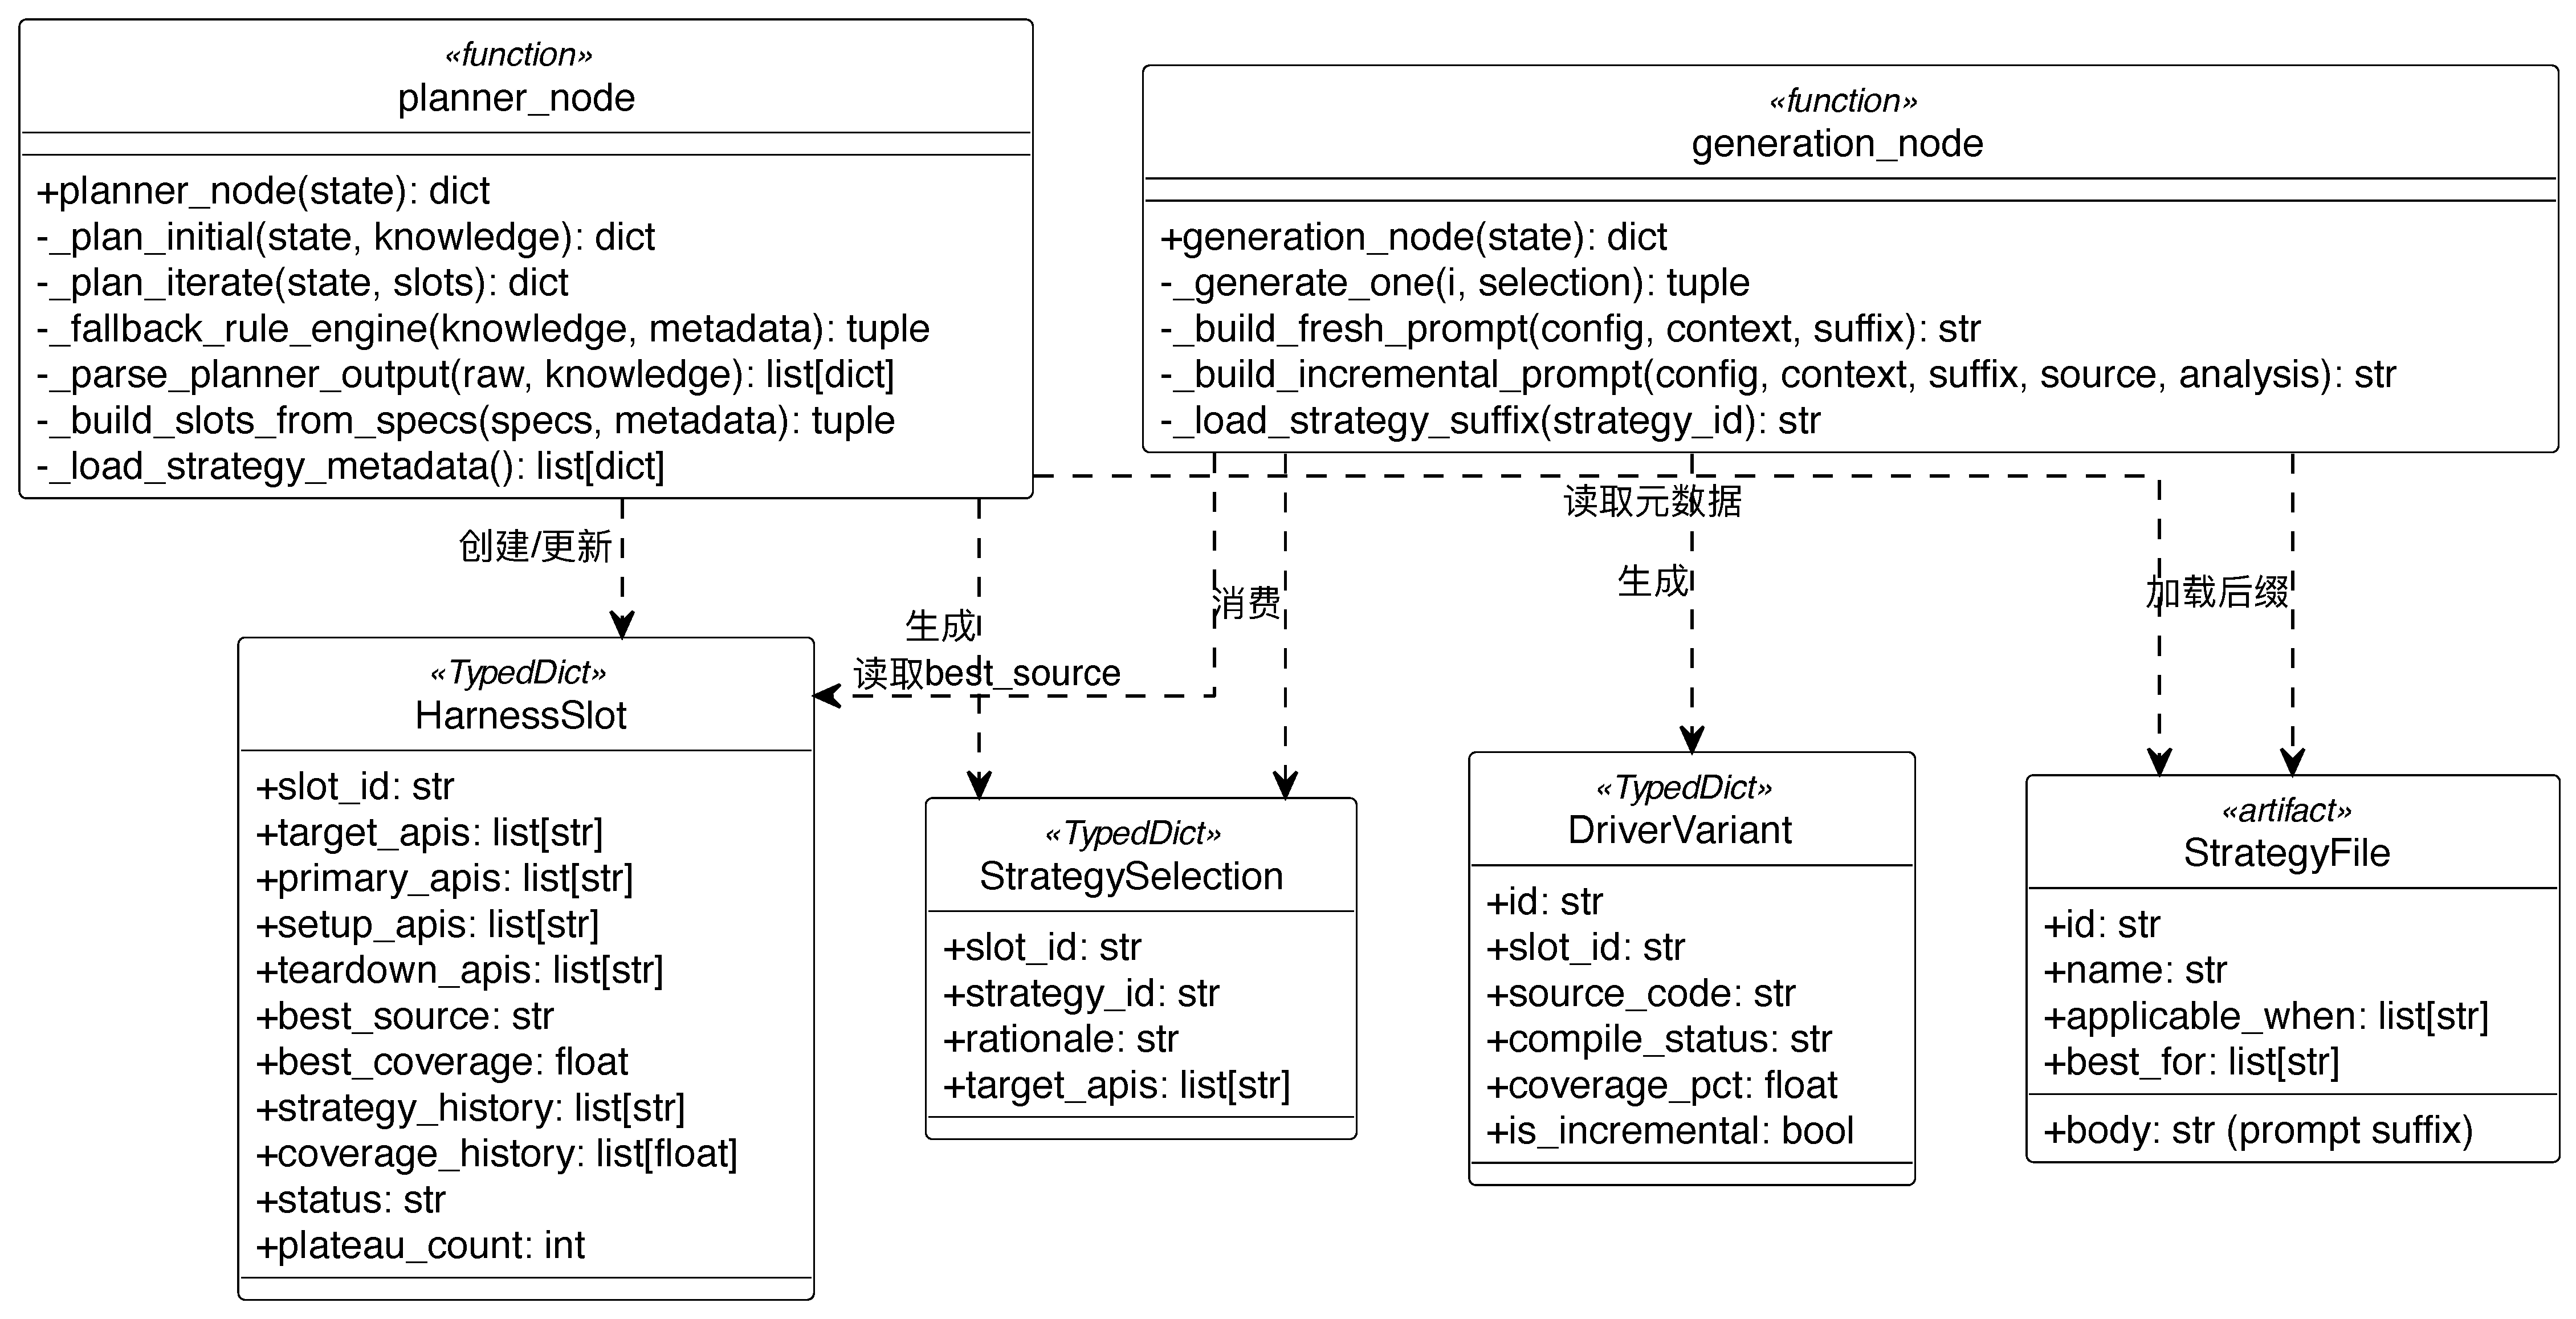
\includegraphics[width=\textwidth]{images/generation_class.pdf}
    \caption{策略规划与代码生成模块详细设计类图}
    \label{fig:generation-class}
\end{figure}

\subsection{策略规划与代码生成模块详细设计}

图\ref{fig:generation-class}展示了策略规划与代码生成模块的详细设计类图。

该模块包含两个核心函数类和四个数据类型。\texttt{planner\_node}函数类封装了策略规划的全部逻辑，公开方法\texttt{planner\_node}作为LangGraph节点入口，内部根据当前轮次分派到\texttt{\_plan\_initial}（探索阶段）或\texttt{\_plan\_iterate}（利用阶段）。\texttt{\_plan\_initial}方法承担探索阶段的核心工作：借助大语言模型进行场景推理。具体做法是将完整的API知识、调用图、类型定义注入提示词模板，由LLM分析API间的语义关系并据此设计测试场景。LLM返回的JSON结构先经\texttt{\_parse\_planner\_output}解析，再由\texttt{\_build\_slots\_from\_specs}转化为具体槽位对象。为防止LLM调用失败导致流水线中断，此处还设置了容错保障，\texttt{\_fallback\_rule\_engine}可接管工作，通过\texttt{GroupingEngine}做确定性降级。

\texttt{generation\_node}函数类封装了代码生成的全部逻辑，通过\texttt{ThreadPoolExecutor}并行调用大语言模型，为每个策略选择生成一个模糊驱动变体。内部区分两种提示词构建路径：\texttt{\_build\_fresh\_prompt}用于首轮从零生成，\texttt{\_build\_incremental\_prompt}用于后续轮次的增量改进。\texttt{\_load\_strategy\_suffix}方法从策略文件中加载YAML前置元数据之后的正文部分，作为提示词的策略后缀。

\texttt{HarnessSlot}是系统的核心状态单元，代表一个独立的模糊测试场景。每个槽位维护目标API集合（分为primary、setup、teardown三类）、历史最佳驱动源码、覆盖率历史、策略切换记录和停滞计数器。\texttt{StrategySelection}记录规划智能体为每个槽位做出的策略决策，包括策略ID、决策理由和目标API列表。\texttt{DriverVariant}记录生成智能体产出的每个驱动变体的完整信息。\texttt{StrategyFile}表示策略库中的策略文件，包含YAML前置元数据（适用条件、最佳场景）和Markdown正文（生成指导）。

图\ref{fig:generation-seq}展示了策略规划与代码生成模块的详细设计顺序图，可以看到探索阶段和利用阶段采用不同的执行路径。

\begin{figure}[H]
    \centering
    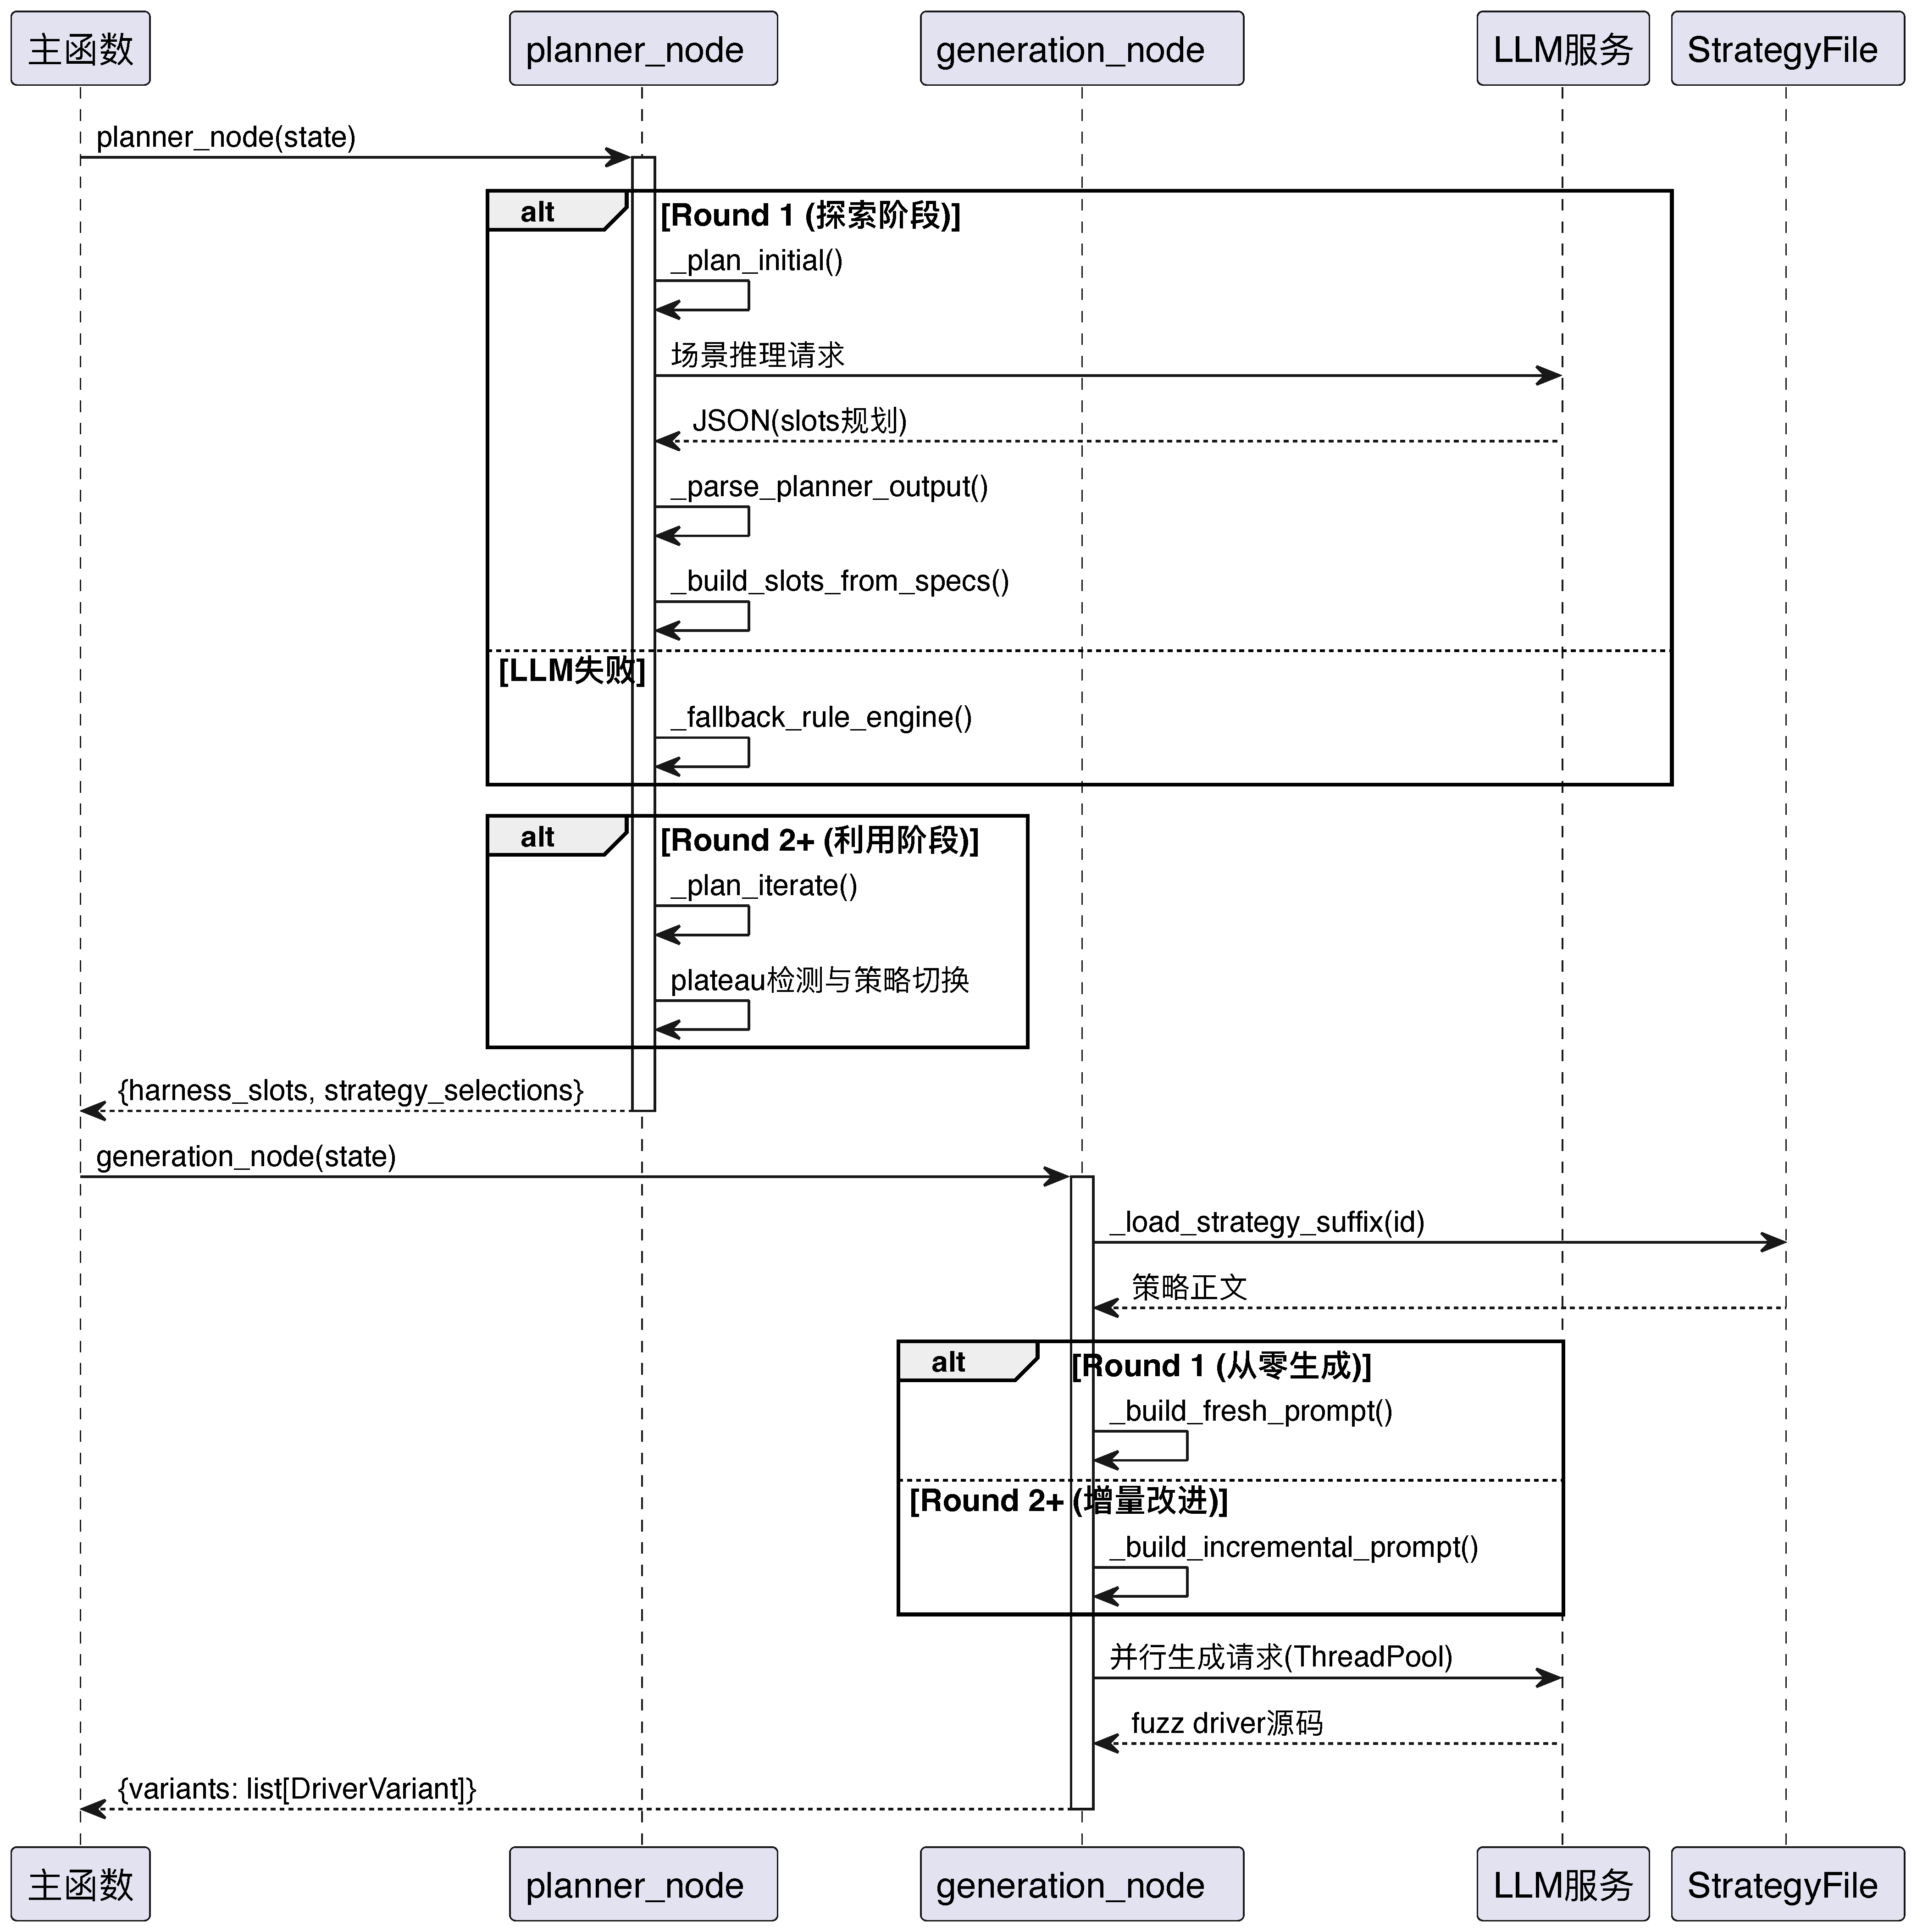
\includegraphics[width=\textwidth]{images/generation_seq.pdf}
    \caption{策略规划与代码生成模块详细设计顺序图}
    \label{fig:generation-seq}
\end{figure}

主函数先调用\texttt{planner\_node}执行策略规划。探索阶段（Round 1）的做法是把完整API知识、调用图和类型定义全部注入提示词模板，让大语言模型做场景推理。LLM返回一个JSON结构，其中包含多个槽位的规划方案。系统对其做解析校验，通过后创建\texttt{HarnessSlot}和\texttt{StrategySelection}对象。若LLM调用因网络超时或返回格式不合法而失败，则降级到规则引擎做确定性分组。进入利用阶段（Round 2+）后，规划逻辑有所不同：遍历所有活跃槽位，依据停滞计数器判断是否需要切换策略。系统设定的阈值是连续两轮覆盖率无提升则切换至\texttt{targeted-expansion}；若连续四轮仍无进展，则标记该槽位已收敛，不再投入计算资源。

随后主函数调用\texttt{generation\_node}启动代码生成。生成智能体先加载对应的策略文件后缀，然后根据当前轮次选择提示词构建路径：首轮使用三部分组装的从零生成提示词，后续轮次使用包含现有代码和诊断约束的增量改进提示词。最终通过线程池并行调用大语言模型，为每个策略选择生成一个模糊驱动变体。

\subsection{探索阶段策略规划功能实现}

这一小节解析策略规划智能体在探索阶段（Round 1）的核心实现。本节依次说明LLM场景推理、输出解析校验和确定性回退机制。

\subsubsection{LLM场景推理}

探索阶段的核心任务是将目标库的API知识转化为若干独立的模糊测试场景。系统将完整的API分类概览、调用图和类型定义注入规划提示词模板，要求大语言模型分析API间的语义关系，设计互不重叠的测试场景，并为每个场景选择最匹配的策略。\texttt{\_plan\_initial}方法的实现如图\ref{fig:plan-initial}所示。

\begin{figure}[H]
    \centering
    \begin{lstlisting}[style=style@python]
   def _plan_initial(state: PipelineState, knowledge: dict) -> dict:
       target_config = state["target_config"]
       lib_name = target_config.get("library_name", "?")
       strategy_metadata = _load_strategy_metadata()
       context = build_planner_context(knowledge, [], strategy_metadata)
       strategies_text = _format_strategies(strategy_metadata)
       prompt = PLANNER_TEMPLATE.replace("{{LIBRARY_NAME}}", lib_name)
       prompt = prompt.replace("{{KNOWLEDGE_CONTEXT}}", context)
       prompt = prompt.replace("{{CALL_GRAPH}}", _format_call_graph(knowledge))
       prompt = prompt.replace("{{TYPE_DEFINITIONS}}", _format_type_defs(knowledge))
       prompt = prompt.replace("{{STRATEGIES}}", strategies_text)
       try:
           llm = create_llm(temperature=max(state.get("temperature", 0.4) - 0.1, 0.1))
           response = llm.invoke([...])
           slot_specs = _parse_planner_output(response.content, knowledge)
           slots, selections = _build_slots_from_specs(slot_specs, strategy_metadata)
       except Exception:
           slots, selections = _fallback_rule_engine(knowledge, strategy_metadata)
       return {"harness_slots": slots, "strategy_selections": selections}
    \end{lstlisting}
    \caption{探索阶段策略规划核心流程}
    \label{fig:plan-initial}
\end{figure}

提示词组装采用模板变量替换机制，将五个知识维度注入固定模板：库名称、API知识上下文、调用图、类型定义和可用策略列表。值得注意的是温度参数的设置，比全局温度低0.1（最低0.1），目的是获得更确定性的规划输出。

\subsubsection{输出解析与校验}

大语言模型返回的规划结果为JSON格式，系统通过\texttt{\_parse\_planner\_output}方法做严格的解析和校验。实现如图\ref{fig:parse-planner}所示。

\begin{figure}[H]
    \centering
    \begin{lstlisting}[style=style@python]
   def _parse_planner_output(raw: str, knowledge: dict) -> list[dict]:
       text = raw.strip()
       match = re.search(r"```(?:json)?\s*\n(.+?)```", text, re.DOTALL)
       if match:
           text = match.group(1).strip()
       data = json.loads(text)
       slots_raw = data.get("slots", [])
       valid_apis = {a["name"] for a in knowledge.get("api_entries", [])}
       valid_strategies = {"parse-centric", "multi-api-sequence",
                           "roundtrip", "targeted-expansion", ...}
       result = []
       for spec in slots_raw:
           primary = [a for a in spec.get("primary_apis", []) if a in valid_apis]
           if not primary:
               continue
           strategy = spec.get("strategy_id", "multi-api-sequence")
           if strategy not in valid_strategies:
               strategy = "multi-api-sequence"
           result.append({...})
       return result
    \end{lstlisting}
    \caption{LLM规划输出解析与校验}
    \label{fig:parse-planner}
\end{figure}

该方法的容错设计体现在多个层面。在格式层面，它兼容两种LLM输出形式，既能从Markdown代码块中提取JSON，也能直接处理纯JSON文本。在语义层面，对API名称做有效性校验，将LLM幻觉产生的不存在函数名过滤掉。在策略层面，对策略ID做合法性检查，遇到无效策略则回退到默认的\texttt{multi-api-sequence}。经过这些校验后，只有至少包含一个有效primary API的槽位才会被保留。

\subsubsection{确定性回退机制}

当LLM调用失败时（无论是网络超时、配额耗尽还是返回格式无法解析），系统降级到基于规则引擎的确定性回退方案。这保证了流水线不会因单次LLM失败而中断。回退机制的实现如图\ref{fig:fallback-engine}所示。

\begin{figure}[H]
    \centering
    \begin{lstlisting}[style=style@python]
   def _fallback_rule_engine(knowledge: dict,
                                  strategy_metadata: list[dict]
                                  ) -> tuple[list[HarnessSlot], list[StrategySelection]]:
       groups = group_apis(knowledge, max_groups=10)
       slots: list[HarnessSlot] = []
       selections: list[StrategySelection] = []
       for i, group in enumerate(groups):
           strategy_id = match_strategy(group, strategy_metadata)
           slot_id = f"slot_{i}"
           slots.append(HarnessSlot(
               slot_id=slot_id, group_id=group["group_id"],
               target_apis=group["apis"], primary_apis=group["apis"],
               strategy_history=[strategy_id], status="active", ...
           ))
           selections.append(StrategySelection(
               slot_id=slot_id, strategy_id=strategy_id,
               target_apis=group["apis"], ...
           ))
       return slots, selections
    \end{lstlisting}
    \caption{确定性回退规则引擎}
    \label{fig:fallback-engine}
\end{figure}

回退方案调用\texttt{GroupingEngine}的\texttt{group\_apis}方法，基于调用图连通分量和参数类型相似性将API聚类为最多10个分组，再通过\texttt{match\_strategy}方法基于规则评分为每个分组匹配最适合的策略。这个方案缺乏LLM的语义推理能力，但保证了确定性和可重复性。

\subsection{多提示词策略驱动生成功能实现}

这一小节深入代码生成智能体的实现，依次说明策略文件的组织方式、三部分提示词的拼装机制以及增量改进生成的做法。

\subsubsection{策略文件结构}

MAGIC4FDG系统的策略库包含10个策略文件，每个文件采用YAML前置元数据加Markdown正文的双层结构。前置元数据定义策略的适用条件和最佳场景，供规划智能体做策略匹配；正文部分包含具体的生成指导，作为提示词后缀注入代码生成请求。表~\ref{tab:strategy-lib}列出了全部10种策略的名称、核心思路和典型适用场景。

\begin{table}[H]
    \centering
    \caption{MAGIC4FDG策略库（10种策略）}
    \makebox[\textwidth]{
    \resizebox{\textwidth}{!}{
    \begin{tabular}{|l|l|l|}
        \hline
        \textbf{策略ID} & \textbf{核心思路} & \textbf{典型适用场景} \\
        \hline
        parse-centric & 将原始模糊字节直接喂给解析API的各种变体 & 解析类库（JSON、XML、图像） \\
        \hline
        roundtrip & 解析→修改→序列化→再解析，验证往返一致性 & 序列化库（JSON、XML、YAML） \\
        \hline
        multi-api-sequence & 链式调用多个API，构造有状态的调用序列 & 数据结构库 \\
        \hline
        structure-aware & 构造符合格式规范的结构化输入 & 输入语法复杂的解析库 \\
        \hline
        stateful & 跨调用维护上下文状态，测试状态机转换 & 加密库（基于上下文的加解密） \\
        \hline
        differential & 对比同一库中不同API实现的行为差异 & 加密库（不同模式、填充方案） \\
        \hline
        targeted-expansion & 基于覆盖率反馈定向扩展未覆盖区域 & 利用阶段的增量改进 \\
        \hline
        error-path & 故意构造非法输入，覆盖错误处理路径 & 错误处理逻辑复杂的库 \\
        \hline
        callback-driven & 注册回调函数并触发事件驱动的执行路径 & 事件驱动型库 \\
        \hline
        resource-boundary & 测试内存/缓冲区边界条件和资源极限 & 压缩/解压缩库 \\
        \hline
    \end{tabular}}}
    \label{tab:strategy-lib}
\end{table}

图\ref{fig:strategy-format}展示了策略文件的结构示例。

\begin{figure}[H]
    \centering
    \begin{lstlisting}[style=style@base]
   ---
   id: parse-centric
   name: Parse-Centric Input Fuzzing
   applicable_when:
     - "library has parsing functions that accept raw bytes"
     - "API includes multiple parse variants"
   best_for:
     - "parser libraries (JSON, XML, image)"
     - "format decoders"
   ---
   ## Strategy: Parse-Centric
   Feed raw fuzz bytes directly to ALL parsing API variants.
   - Call every parse function variant
   - Use different option flag combinations
   - Exercise error paths by feeding malformed data
   - Use FuzzedDataProvider to split input
    \end{lstlisting}
    \caption{策略文件结构示例（parse-centric）}
    \label{fig:strategy-format}
\end{figure}

系统通过\texttt{\_load\_strategy\_suffix}方法加载策略正文。该方法遍历策略目录下的所有Markdown文件，通过匹配\texttt{id}字段定位目标策略，然后截取YAML前置元数据结束标记（第二个\texttt{‘---’}）之后的全部内容作为策略后缀。

\subsubsection{从零生成提示词组装}

首轮生成采用三部分组装机制构建提示词：基础模板提供通用的生成框架和约束，知识上下文提供目标API的详细信息，策略后缀提供特定策略的生成指导。\texttt{\_build\_fresh\_prompt}方法的实现如图\ref{fig:fresh-prompt}所示。

\begin{figure}[H]
    \centering
    \begin{lstlisting}[style=style@python]
   def _build_fresh_prompt(target_config: dict, knowledge_context: str,
                                strategy_suffix: str) -> str:
       include_dirs = target_config.get("include_dirs", [])
       prompt = (
           GENERATION_TEMPLATE
           .replace("{{LIBRARY_NAME}}", target_config.get("library_name", ""))
           .replace("{{LANGUAGE}}", target_config.get("language", "C"))
           .replace("{{HEADER}}", target_config.get("header", ""))
           .replace("{{INCLUDE_DIRS}}", ", ".join(include_dirs))
           .replace("{{RESEARCH_SUMMARY}}", knowledge_context)
           .replace("{{COVERAGE_FEEDBACK}}", "(first round)")
       )
       if strategy_suffix:
           prompt += "\n\n" + strategy_suffix
       return prompt
    \end{lstlisting}
    \caption{从零生成提示词三部分组装}
    \label{fig:fresh-prompt}
\end{figure}

基础模板\texttt{GENERATION\_TEMPLATE}对模糊驱动提出了若干通用约束：必须包含\texttt{LLVMFuzzerTestOneInput}入口函数，头文件引用路径正确，资源管理需满足内存安全。知识上下文由\texttt{build\_generator\_context}方法构建，涵盖目标API的完整签名、参数语义、类型定义和宏常量。策略后缀则给出特定测试策略的具体指导，以\texttt{parse-centric}策略为例，它会要求"把原始模糊字节直接喂给所有解析API变体"。三部分各有侧重，拼合后形成完整的生成请求。

\subsubsection{增量改进提示词组装}

第二轮及之后的迭代采用增量改进模式，基于该槽位的历史最佳驱动做修改，而非从零重新生成。这样做的好处是保留了已有的覆盖率成果，同时针对诊断智能体识别的覆盖率缺口做定向改进。\texttt{\_build\_incremental\_prompt}方法的实现如图\ref{fig:incremental-prompt}所示。

\begin{figure}[H]
    \centering
    \begin{lstlisting}[style=style@python]
   def _build_incremental_prompt(target_config: dict, knowledge_context: str,
                                       strategy_suffix: str, base_source: str,
                                       coverage_analysis: dict) -> str:
       constraints_text = ""
       if coverage_analysis:
           constraints = coverage_analysis.get("constraints", [])
           if constraints:
               constraints_text = "\n".join(
                   f"- {c.get('target', '?')}: {c.get('precondition', '')}"
                   for c in constraints[:10])
       clusters_text = ""
       if coverage_analysis:
           clusters = coverage_analysis.get("uncovered_clusters", [])
           if clusters:
               clusters_text = "\n".join(
                   f"- {', '.join(c.get('functions', []))}: {c.get('root_cause', '')}"
                   for c in clusters[:5])
       prompt = f"""## Task: Improve Fuzz Driver
                      ## Current Driver (to be improved)
                      ```cpp
                      {base_source}
                      ```
                      ## Analyst Constraints
                      {constraints_text or "(no specific constraints)"}
                      ## Uncovered Code Clusters
                      {clusters_text or "(no cluster data)"}
                      ## API Knowledge
                      {knowledge_context}
                      ## Strategy Guidance
                      {strategy_suffix}"""
       return prompt
    \end{lstlisting}
    \caption{增量改进提示词组装}
    \label{fig:incremental-prompt}
\end{figure}

增量提示词分五个层次组织信息。最上面放现有驱动源码，作为修改的基础。然后是诊断约束，最多放10条，每条指明需要覆盖的具体目标和前置条件。接着是未覆盖代码簇，最多5个，附带根因分析。再往下是API知识上下文和策略指导。提示词中明确指定了"保留现有驱动中有效的部分，仅添加新的代码路径"，这一步至关重要，否则大语言模型容易将已有的覆盖率成果破坏。

\section{模糊测试与覆盖率收集模块详细设计与实现}

模糊测试与覆盖率收集模块构成了MAGIC4FDG系统的执行层与反馈源。它负责在Docker容器内运行生成的模糊驱动、收集细粒度代码覆盖率数据，并借助控制流图可达性分析剔除结构性不可达的代码路径。该模块的输出直接驱动系统的迭代决策——覆盖率提升则继续优化，停滞则切换策略或终止。本节先通过类图和顺序图阐述模块的详细设计，再分别解析Fork模式模糊测试与语料库重放、控制流图可达性分析两个核心功能的实现。

\subsection{模糊测试与覆盖率收集模块详细设计}

图\ref{fig:coverage-class}展示了模糊测试与覆盖率收集模块的详细设计类图。

\begin{figure}[H]
    \centering
    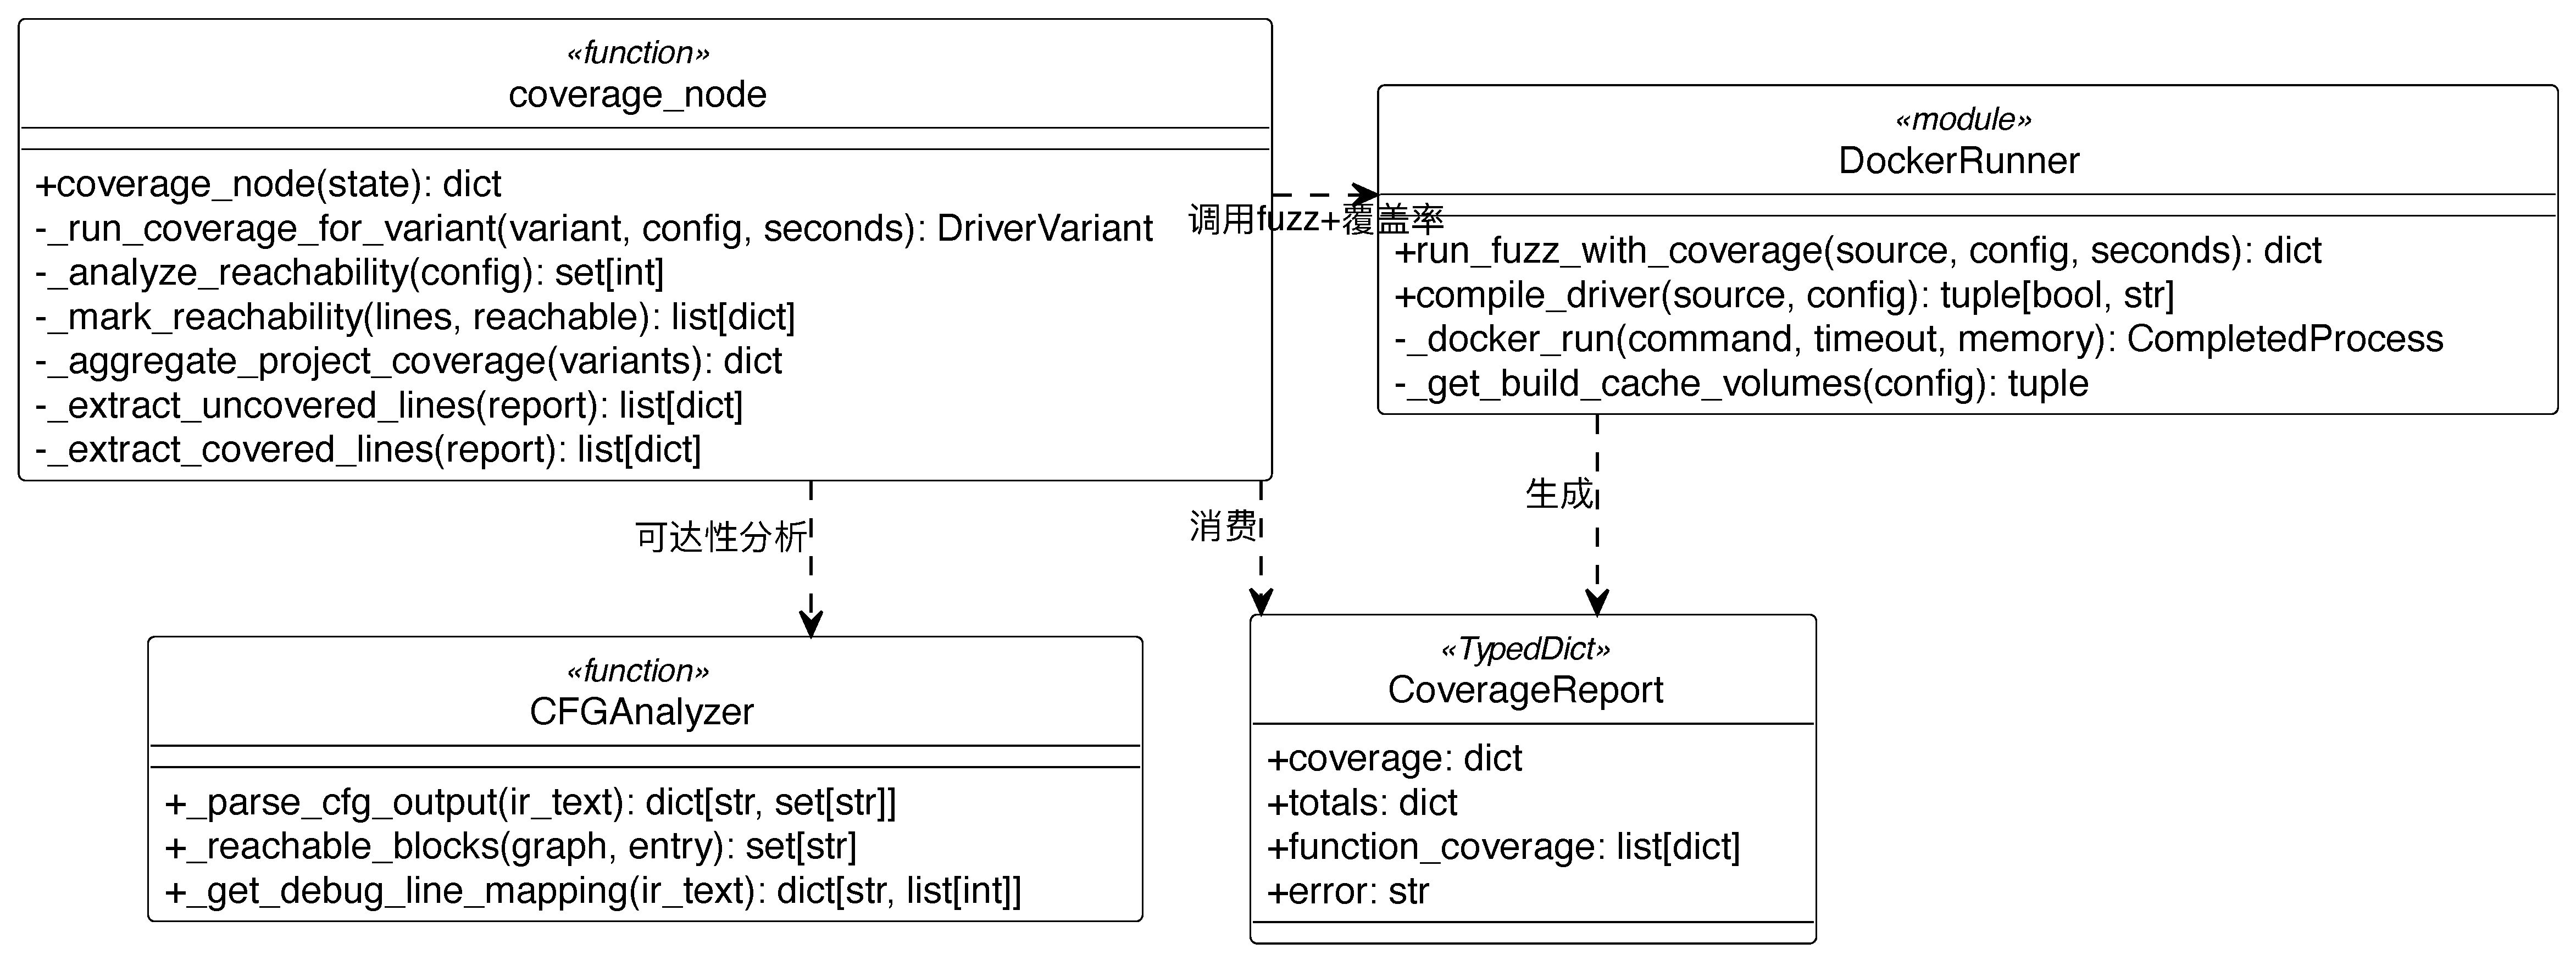
\includegraphics[width=\textwidth]{images/coverage_class.pdf}
    \caption{模糊测试与覆盖率收集模块详细设计类图}
    \label{fig:coverage-class}
\end{figure}

该模块包含三个核心组件，各负责一项独立职能。\texttt{coverage\_node}函数类是LangGraph节点入口，它编排整个流程：先执行可达性分析获取可达行集合，然后开启线程池并行对所有编译成功的变体做模糊测试，最后更新各槽位的覆盖率状态、聚合出项目级覆盖率。\texttt{DockerRunner}模块封装了Docker容器内的全部执行操作，核心方法\texttt{run\_fuzz\_with\_coverage}采用从编译到覆盖率导出的完整八步流水线。\texttt{CFGAnalyzer}组件负责基于LLVM IR的控制流图可达性分析，内部拆分为CFG解析、BFS遍历、调试信息行号映射三个子功能。

\texttt{CoverageReport}记录单个变体的覆盖率收集结果，包含行覆盖率、分支覆盖率、函数覆盖率和未覆盖行列表。值得注意的是，每个未覆盖行条目都附带一个\texttt{reachable}字段，标明该行从驱动入口函数出发是否结构性可达。

图\ref{fig:coverage-seq}展示了模糊测试与覆盖率收集模块的详细设计顺序图。

\begin{figure}[H]
    \centering
    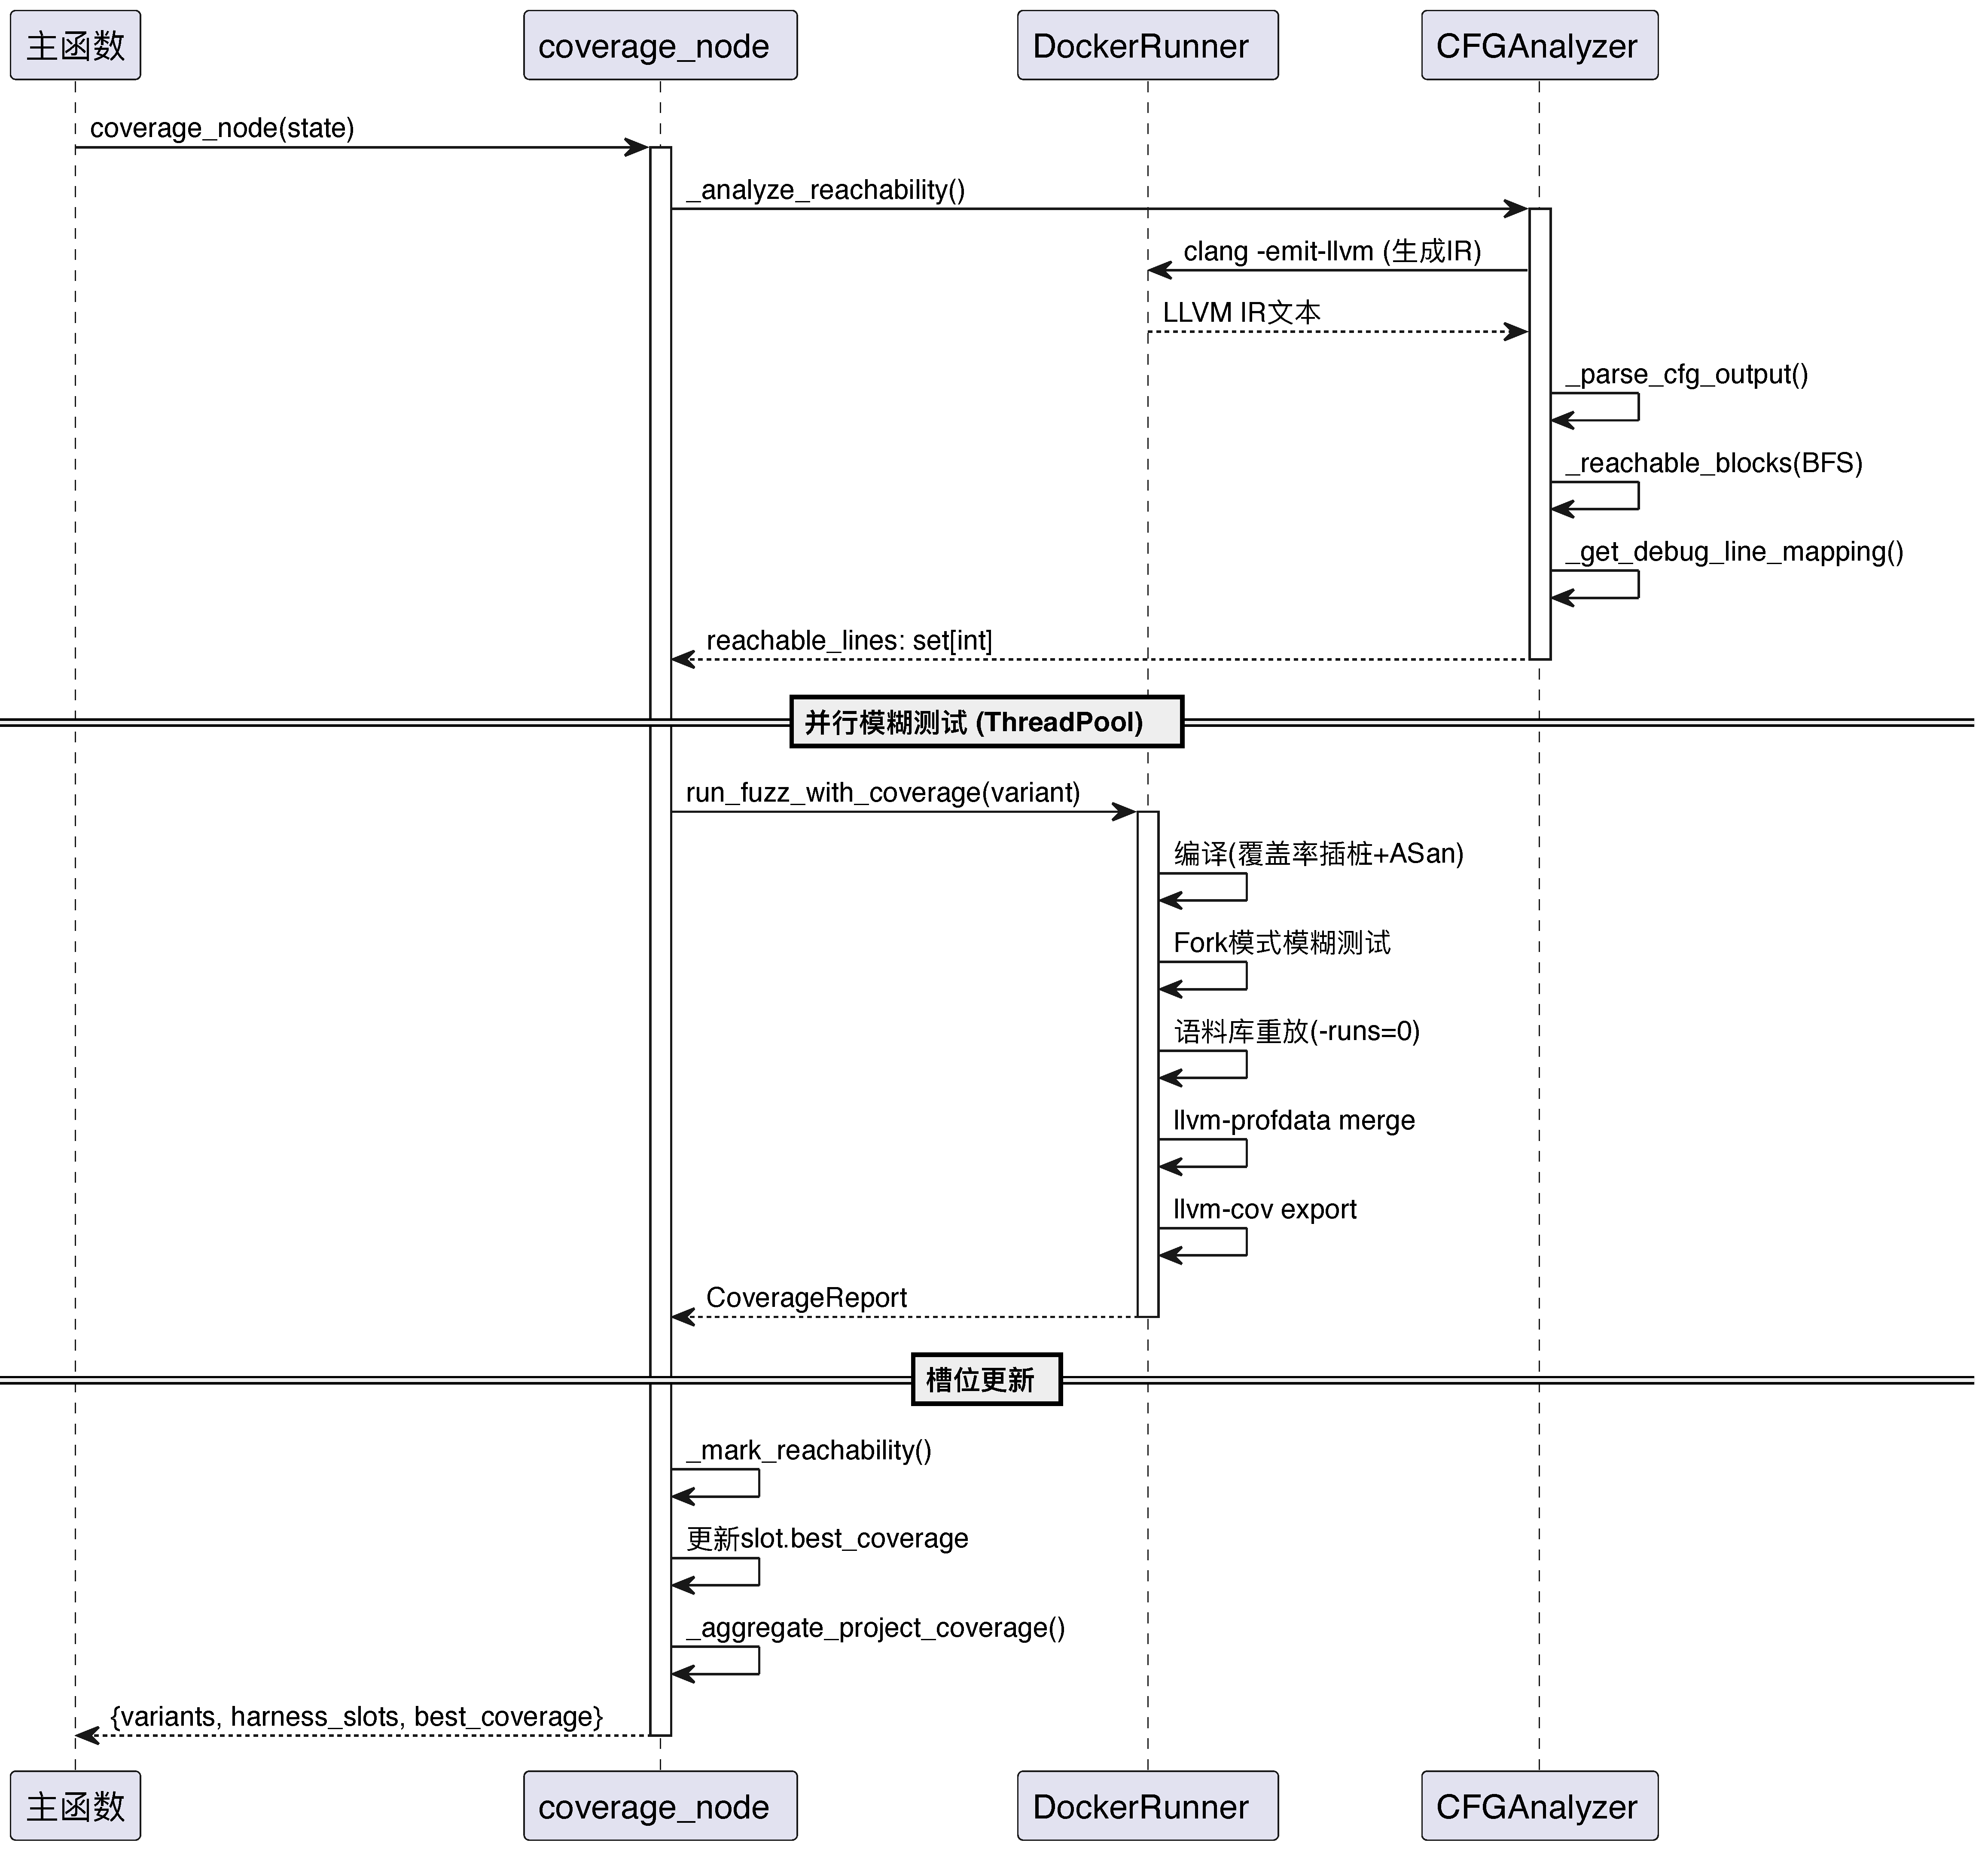
\includegraphics[width=\textwidth]{images/coverage_seq.pdf}
    \caption{模糊测试与覆盖率收集模块详细设计顺序图}
    \label{fig:coverage-seq}
\end{figure}

主函数调用\texttt{coverage\_node}后，流程分为两大步骤。第一步是可达性分析：在Docker容器内用\texttt{clang -emit-llvm}生成LLVM IR，解析IR文本构建控制流图，从入口块执行BFS获取可达基本块集合，再通过调试信息将可达块映射回源码行号。第二步是实际的模糊测试：节点开启线程池，并行调用\texttt{DockerRunner}的\texttt{run\_fuzz\_with\_coverage}方法，每个编译成功的变体都经历完整的八步流水线。执行完毕后，节点为每个未覆盖行标注可达性信息，更新各槽位的最佳覆盖率和停滞计数器，最后将所有槽位覆盖行取并集计算出项目级覆盖率。

\subsection{Fork模式模糊测试与语料库重放功能实现}

这一小节解析\texttt{run\_fuzz\_with\_coverage}方法实现的八步覆盖率收集流水线。本节重点说明Fork模式崩溃隔离和语料库重放的设计动机与实现细节。

\subsubsection{八步流水线设计}

覆盖率收集流水线在单个Docker容器内依次执行八个步骤，其核心流程如图\ref{fig:fuzz-pipeline}所示。

\begin{figure}[H]
    \centering
    \begin{lstlisting}[style=style@base]
   # Step 1: 编译(覆盖率插桩 + ASan)
   COMMON_FLAGS="-g -O1 -fprofile-instr-generate -fcoverage-mapping
                 -fsanitize=address"
   clang++ $COMMON_FLAGS driver.cpp -fsanitize=fuzzer,address -o fuzz_cov

   # Step 2: 准备语料库(种子 + 累积)
   mkdir -p /tmp/corpus && cp seed_corpus/* /tmp/corpus/
   cp accumulated_corpus/* /tmp/corpus/

   # Step 3: Fork模式模糊测试(崩溃隔离)
   export ASAN_OPTIONS=halt_on_error=0:exitcode=0:detect_leaks=0
   ./fuzz_cov /tmp/corpus -max_total_time=60 -fork=1

   # Step 4: 保存累积语料库
   cp /tmp/corpus/* accumulated_corpus/

   # Step 5: 语料库重放(无Fork, 收集完整profraw)
   export LLVM_PROFILE_FILE=/tmp/replay_%m.profraw
   ./fuzz_cov /tmp/corpus -runs=0

   # Step 6: 合并覆盖率数据
   llvm-profdata merge -sparse /tmp/replay_*.profraw -o fuzzer.profdata

   # Step 7: 导出覆盖率报告(JSON)
   llvm-cov export ./fuzz_cov -instr-profile=fuzzer.profdata sources

   # Step 8: 导出函数级报告
   llvm-cov report ./fuzz_cov -instr-profile=fuzzer.profdata sources
    \end{lstlisting}
    \caption{八步覆盖率收集流水线}
    \label{fig:fuzz-pipeline}
\end{figure}

\subsubsection{Fork模式崩溃隔离}

LibFuzzer的Fork模式（\texttt{-fork=1}）将每个模糊输入在独立子进程中执行。当AddressSanitizer检测到内存错误时，仅子进程被终止，主进程继续运行后续输入。这一机制对覆盖率收集至关重要，若不使用Fork模式，单次ASan崩溃就会终止整个模糊测试进程，后续输入无法执行，覆盖率数据严重不完整。系统同时设置\texttt{ASAN\_OPTIONS=halt\_on\_error=0:exitcode=0:detect\_leaks=0}，确保即使在非Fork模式的重放阶段，ASan错误也不会中断执行。

\subsubsection{语料库重放设计动机}

Fork模式存在一个固有缺陷：子进程在超时时被\texttt{SIGKILL}强制终止，\texttt{profraw}覆盖率数据文件来不及刷新到磁盘。这一技术细节需要说明：Fork模式下子进程超时会被\texttt{SIGKILL}强制终止，\texttt{profraw}覆盖率文件无法正常落盘。因此系统在Fork模式执行完毕后，额外增加了一次无Fork模式的语料库重放（\texttt{-runs=0}）。重放阶段使用独立的\texttt{LLVM\_PROFILE\_FILE}路径，\texttt{llvm-profdata merge}合并时优先取重放产生的完整数据。本质上这是"先Fork后重放"的两阶段设计，Fork保证崩溃不会打断测试，重放保证覆盖率数据的完整性。

另外系统还做了跨轮次的语料库累积：每轮测试结束后把新发现的语料库文件存到持久化目录，下一轮启动时自动加载作为初始种子。这样后续轮次就能在前面的探索基础上继续深入，不用重复走已知路径。

\subsection{控制流图可达性分析功能实现}

这一小节解析基于LLVM IR的控制流图可达性分析实现。该分析用于过滤结构性不可达的未覆盖代码行，避免诊断智能体在无法通过任何输入触达的代码路径上浪费推理资源。

\subsubsection{LLVM IR生成与CFG解析}

可达性分析的第一步是在Docker容器内通过\texttt{clang -S -emit-llvm -g -O0}将目标源文件编译为LLVM中间表示（IR），保留完整的调试信息。然后系统解析IR文本构建控制流图。CFG解析的核心实现如图\ref{fig:parse-cfg}所示。

\begin{figure}[H]
    \centering
    \begin{lstlisting}[style=style@python]
   def _parse_cfg_output(cfg_text: str) -> dict[str, set[str]]:
       graph: dict[str, set[str]] = {}
       current_block = None
       for line in cfg_text.splitlines():
           block_match = re.match(r"^(\S+):.*$", line.strip())
           if block_match:
               current_block = block_match.group(1)
               if current_block not in graph:
                   graph[current_block] = set()
               continue
           if current_block:
               br_match = re.match(r"\s*br\s+.*label\s+%(\S+)", line)
               if br_match:
                   targets = re.findall(r"label\s+%([A-Za-z0-9_.]+)", line)
                   for t in targets:
                       graph[current_block].add(t)
                       if t not in graph:
                           graph[t] = set()
       return graph
    \end{lstlisting}
    \caption{LLVM IR控制流图解析}
    \label{fig:parse-cfg}
\end{figure}

该方法逐行扫描LLVM IR文本，通过正则表达式识别两类关键结构：基本块标签（行首非空白字符后跟冒号）和分支指令（\texttt{br}指令中的\texttt{label}目标）。解析结果为邻接表形式的有向图，每个节点为基本块标签，边表示控制流转移关系。

\subsubsection{BFS可达性遍历与行号映射}

获取CFG后，系统从入口基本块出发执行广度优先搜索，确定所有从程序入口可达的基本块。然后通过LLVM IR中的\texttt{!dbg}调试元数据，将可达基本块映射到对应的源码行号。可达性分析的完整流程如图\ref{fig:reachability}所示。

\texttt{\_get\_debug\_line\_mapping}方法通过两阶段处理建立基本块到源码行的映射。第一阶段扫描IR末尾的\texttt{!DILocation}元数据定义，建立元数据ID到行号的索引。第二阶段遍历函数体中每条指令的\texttt{!dbg}引用，将行号归属到对应的基本块。最终，\texttt{\_mark\_reachability}方法将可达性信息标注到每个未覆盖行条目的\texttt{reachable}字段中。诊断智能体仅对\texttt{reachable=True}的未覆盖行做分析，有效避免了在死代码和编译器生成的不可达路径上浪费推理资源。

\begin{figure}[H]
    \centering
    \begin{lstlisting}[style=style@python]
   def _analyze_reachability(target_config: dict) -> set[int]:
       source_files = target_config.get("source_files", [])
       if not source_files:
           return set()
       primary_source = source_files[0]
       include_args = " ".join(f"-I{d}" for d in target_config.get("include_dirs", []))
       # Docker内生成LLVM IR
       result = _docker_run(["bash", "reachability_analysis.sh"])
       ir_text = result.stdout
       # 解析CFG并执行BFS
       graph = _parse_cfg_output(ir_text)
       entry = "entry" if "entry" in graph else next(iter(graph), "")
       reachable = _reachable_blocks(graph, entry)
       # 映射到源码行号
       block_to_lines = _get_debug_line_mapping(ir_text)
       reachable_lines: set[int] = set()
       for block_label in reachable:
           reachable_lines.update(block_to_lines.get(block_label, []))
       return reachable_lines
    \end{lstlisting}
    \caption{控制流图可达性分析完整流程}
    \label{fig:reachability}
\end{figure}

\section{缺口诊断模块详细设计与实现}

缺口诊断模块在整个迭代闭环中承担的职责是诊断覆盖率缺口。它分析每个槽位的覆盖率数据，识别哪些代码未被覆盖以及未覆盖的原因，然后输出结构化的改进约束供下一轮代码生成使用。设计中遵循的一个核心原则是按槽位隔离：每个槽位只分析自身职责范围内的覆盖率，不涉及其他槽位的内容。这样做是为了避免跨槽位的错误引导，比如解析场景的诊断结果不应影响生命周期管理场景的生成。本节先用类图和顺序图说明设计，再分别展开覆盖率缺口诊断和跨轮次知识累积的实现。

\subsection{缺口诊断模块详细设计}

图\ref{fig:analyst-class}展示了缺口诊断模块的详细设计类图。

\texttt{analyst\_node}函数类是模块的驱动核心，其公开方法作为LangGraph节点入口，内部借助线程池对每个活跃槽位并行调用\texttt{\_analyze\_single\_slot}方法完成独立诊断。诊断过程中，\texttt{ContextBuilder}模块负责构建诊断上下文，\texttt{\_build\_uncovered\_summary}和\texttt{\_build\_function\_summary}两个辅助方法则将覆盖率数据转换为大语言模型可理解的文本形式。LLM返回的文本由\texttt{\_parse\_analyst\_response}方法提取其中的JSON结构化分析结果。

\begin{figure}[H]
    \centering
    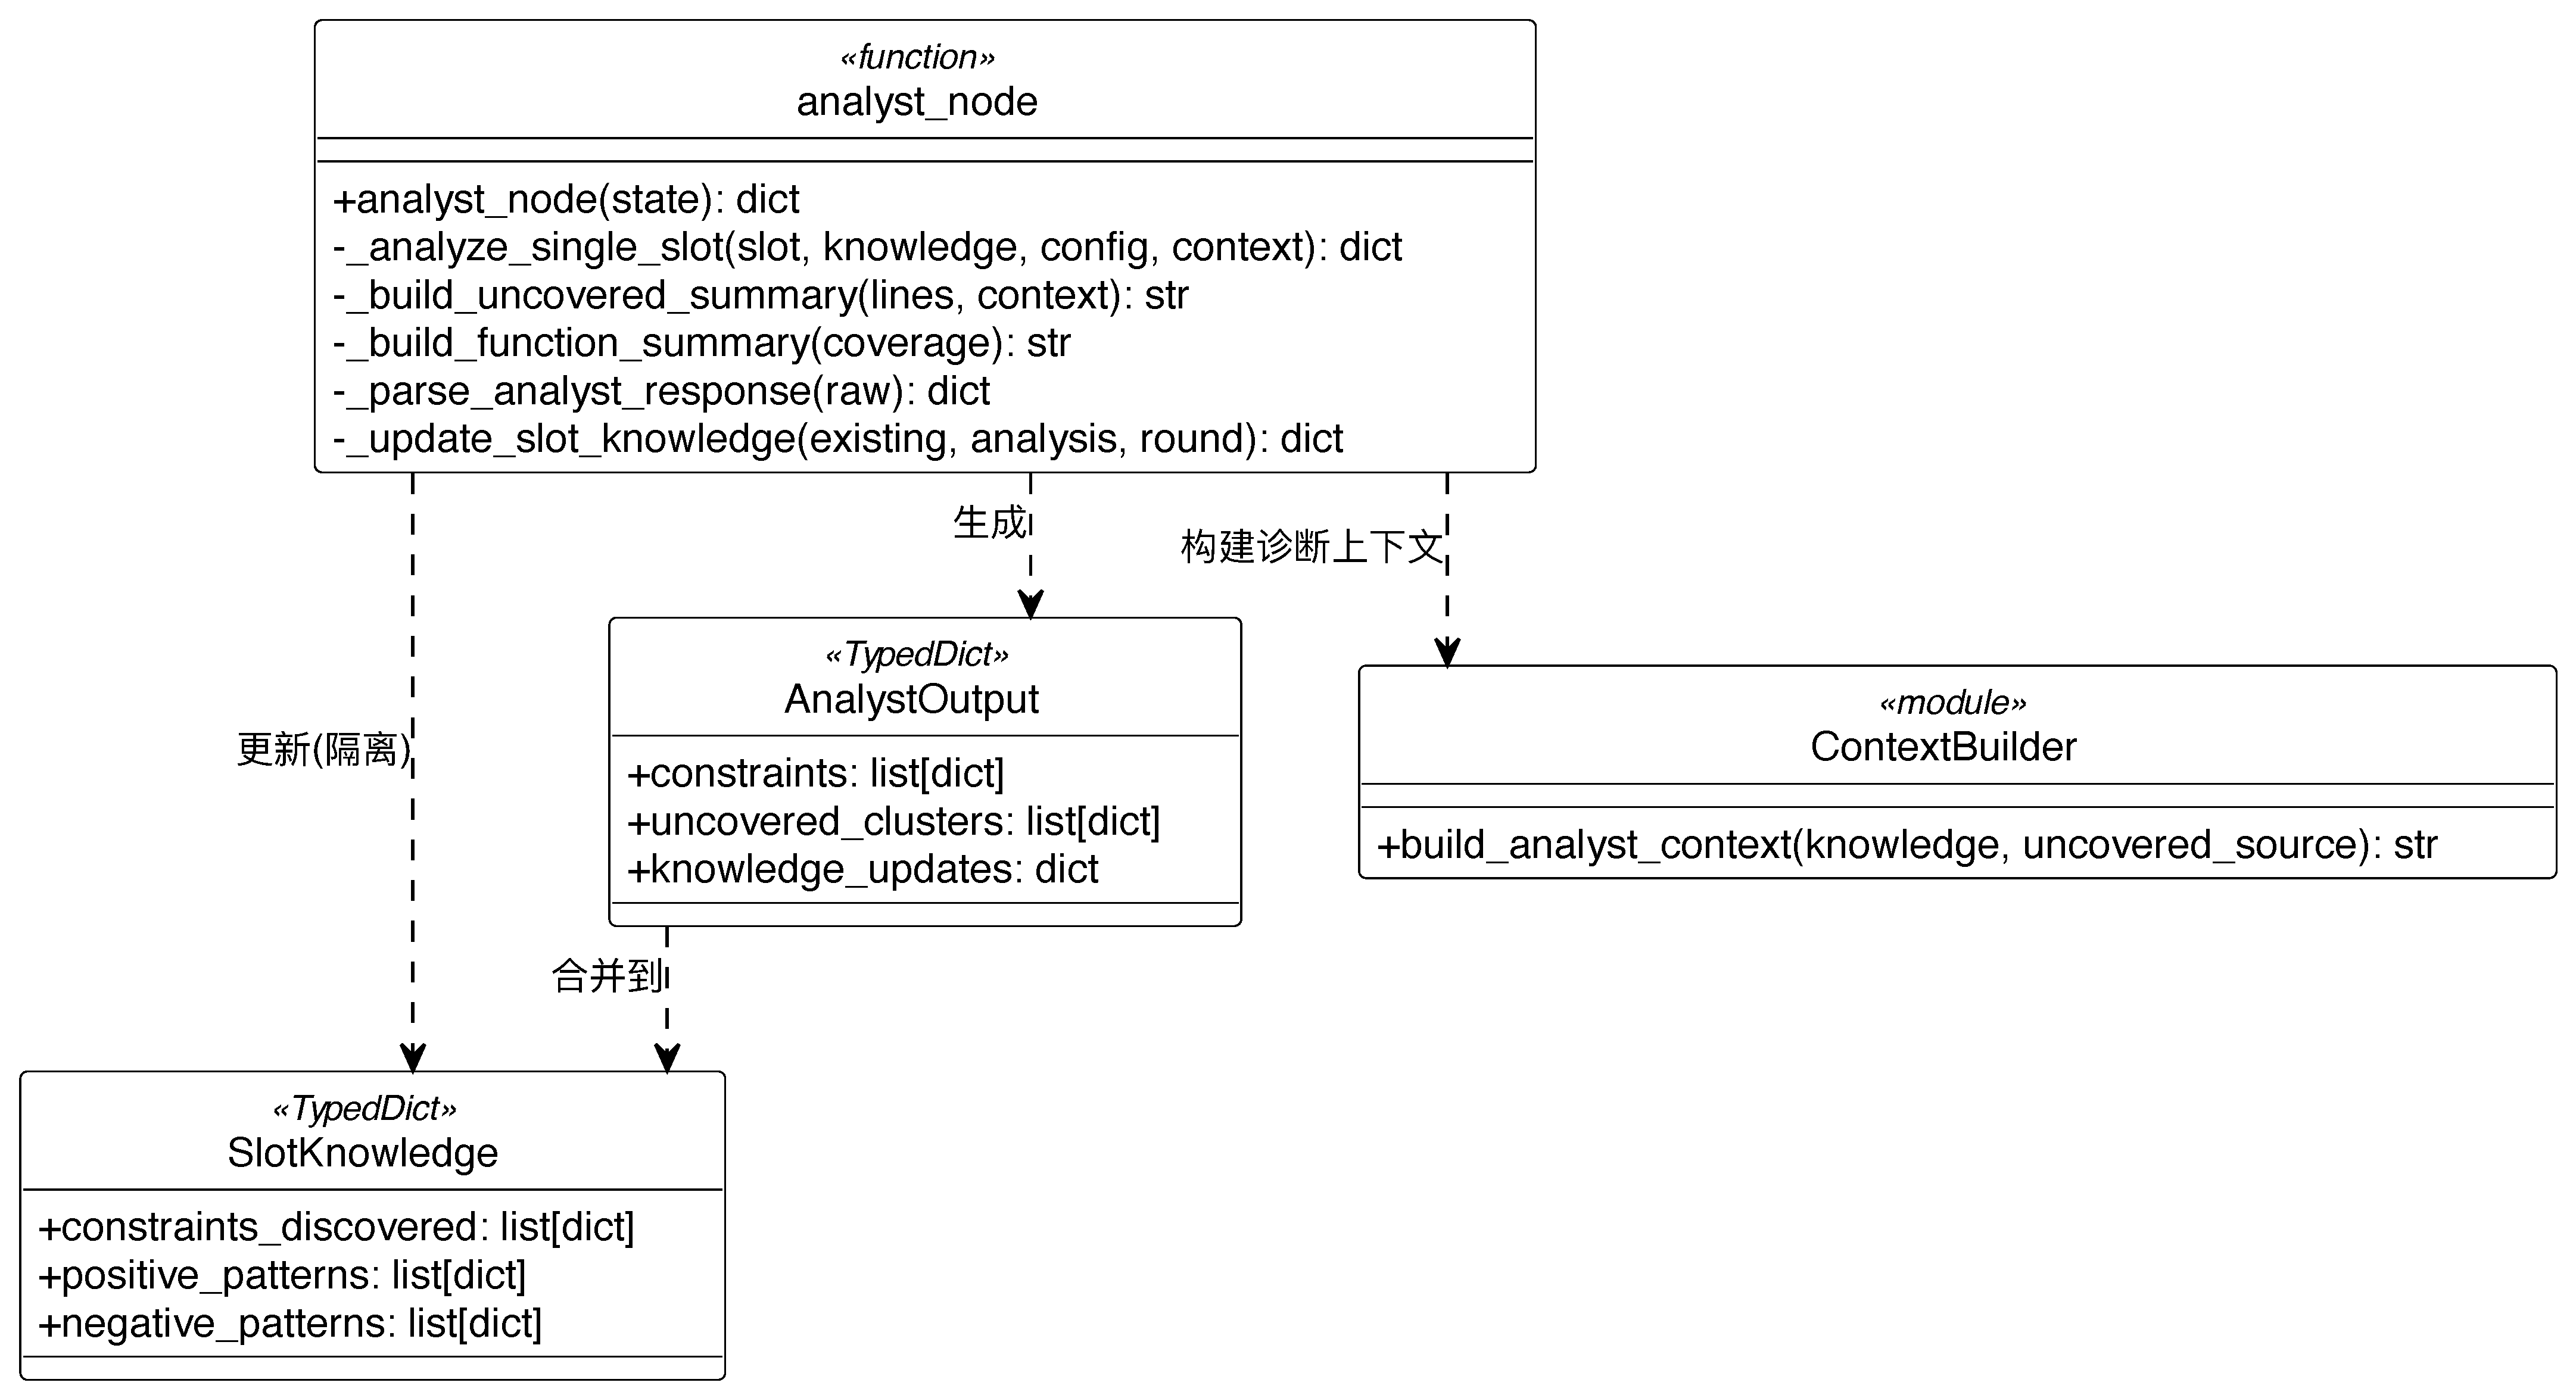
\includegraphics[width=\textwidth]{images/analyst_class.pdf}
    \caption{缺口诊断模块详细设计类图}
    \label{fig:analyst-class}
\end{figure}

\texttt{AnalystOutput}记录单次诊断的输出，包含三个字段：\texttt{constraints}列出需要满足的前置条件和目标API；\texttt{uncovered\_clusters}将未覆盖行按根因聚类；\texttt{knowledge\_updates}包含本轮发现的新约束和模式。\texttt{SlotKnowledge}是每个槽位的隔离知识空间，累积存储历史轮次发现的约束、正向模式和负向模式，供后续轮次的代码生成智能体参考。

图\ref{fig:analyst-seq}展示了缺口诊断模块的详细设计顺序图。

主函数调用\texttt{analyst\_node}启动诊断流程。该节点先筛选所有状态为\texttt{active}的槽位，然后通过线程池并行执行每个槽位的独立分析。对于每个槽位，系统构建包含完整API清单和未覆盖源码行的诊断上下文，组装诊断提示词后调用大语言模型做推理，解析返回的JSON结构化结果。最后，系统将诊断发现合并到该槽位的隔离知识空间中，并递增轮次计数器。

\begin{figure}[H]
    \centering
    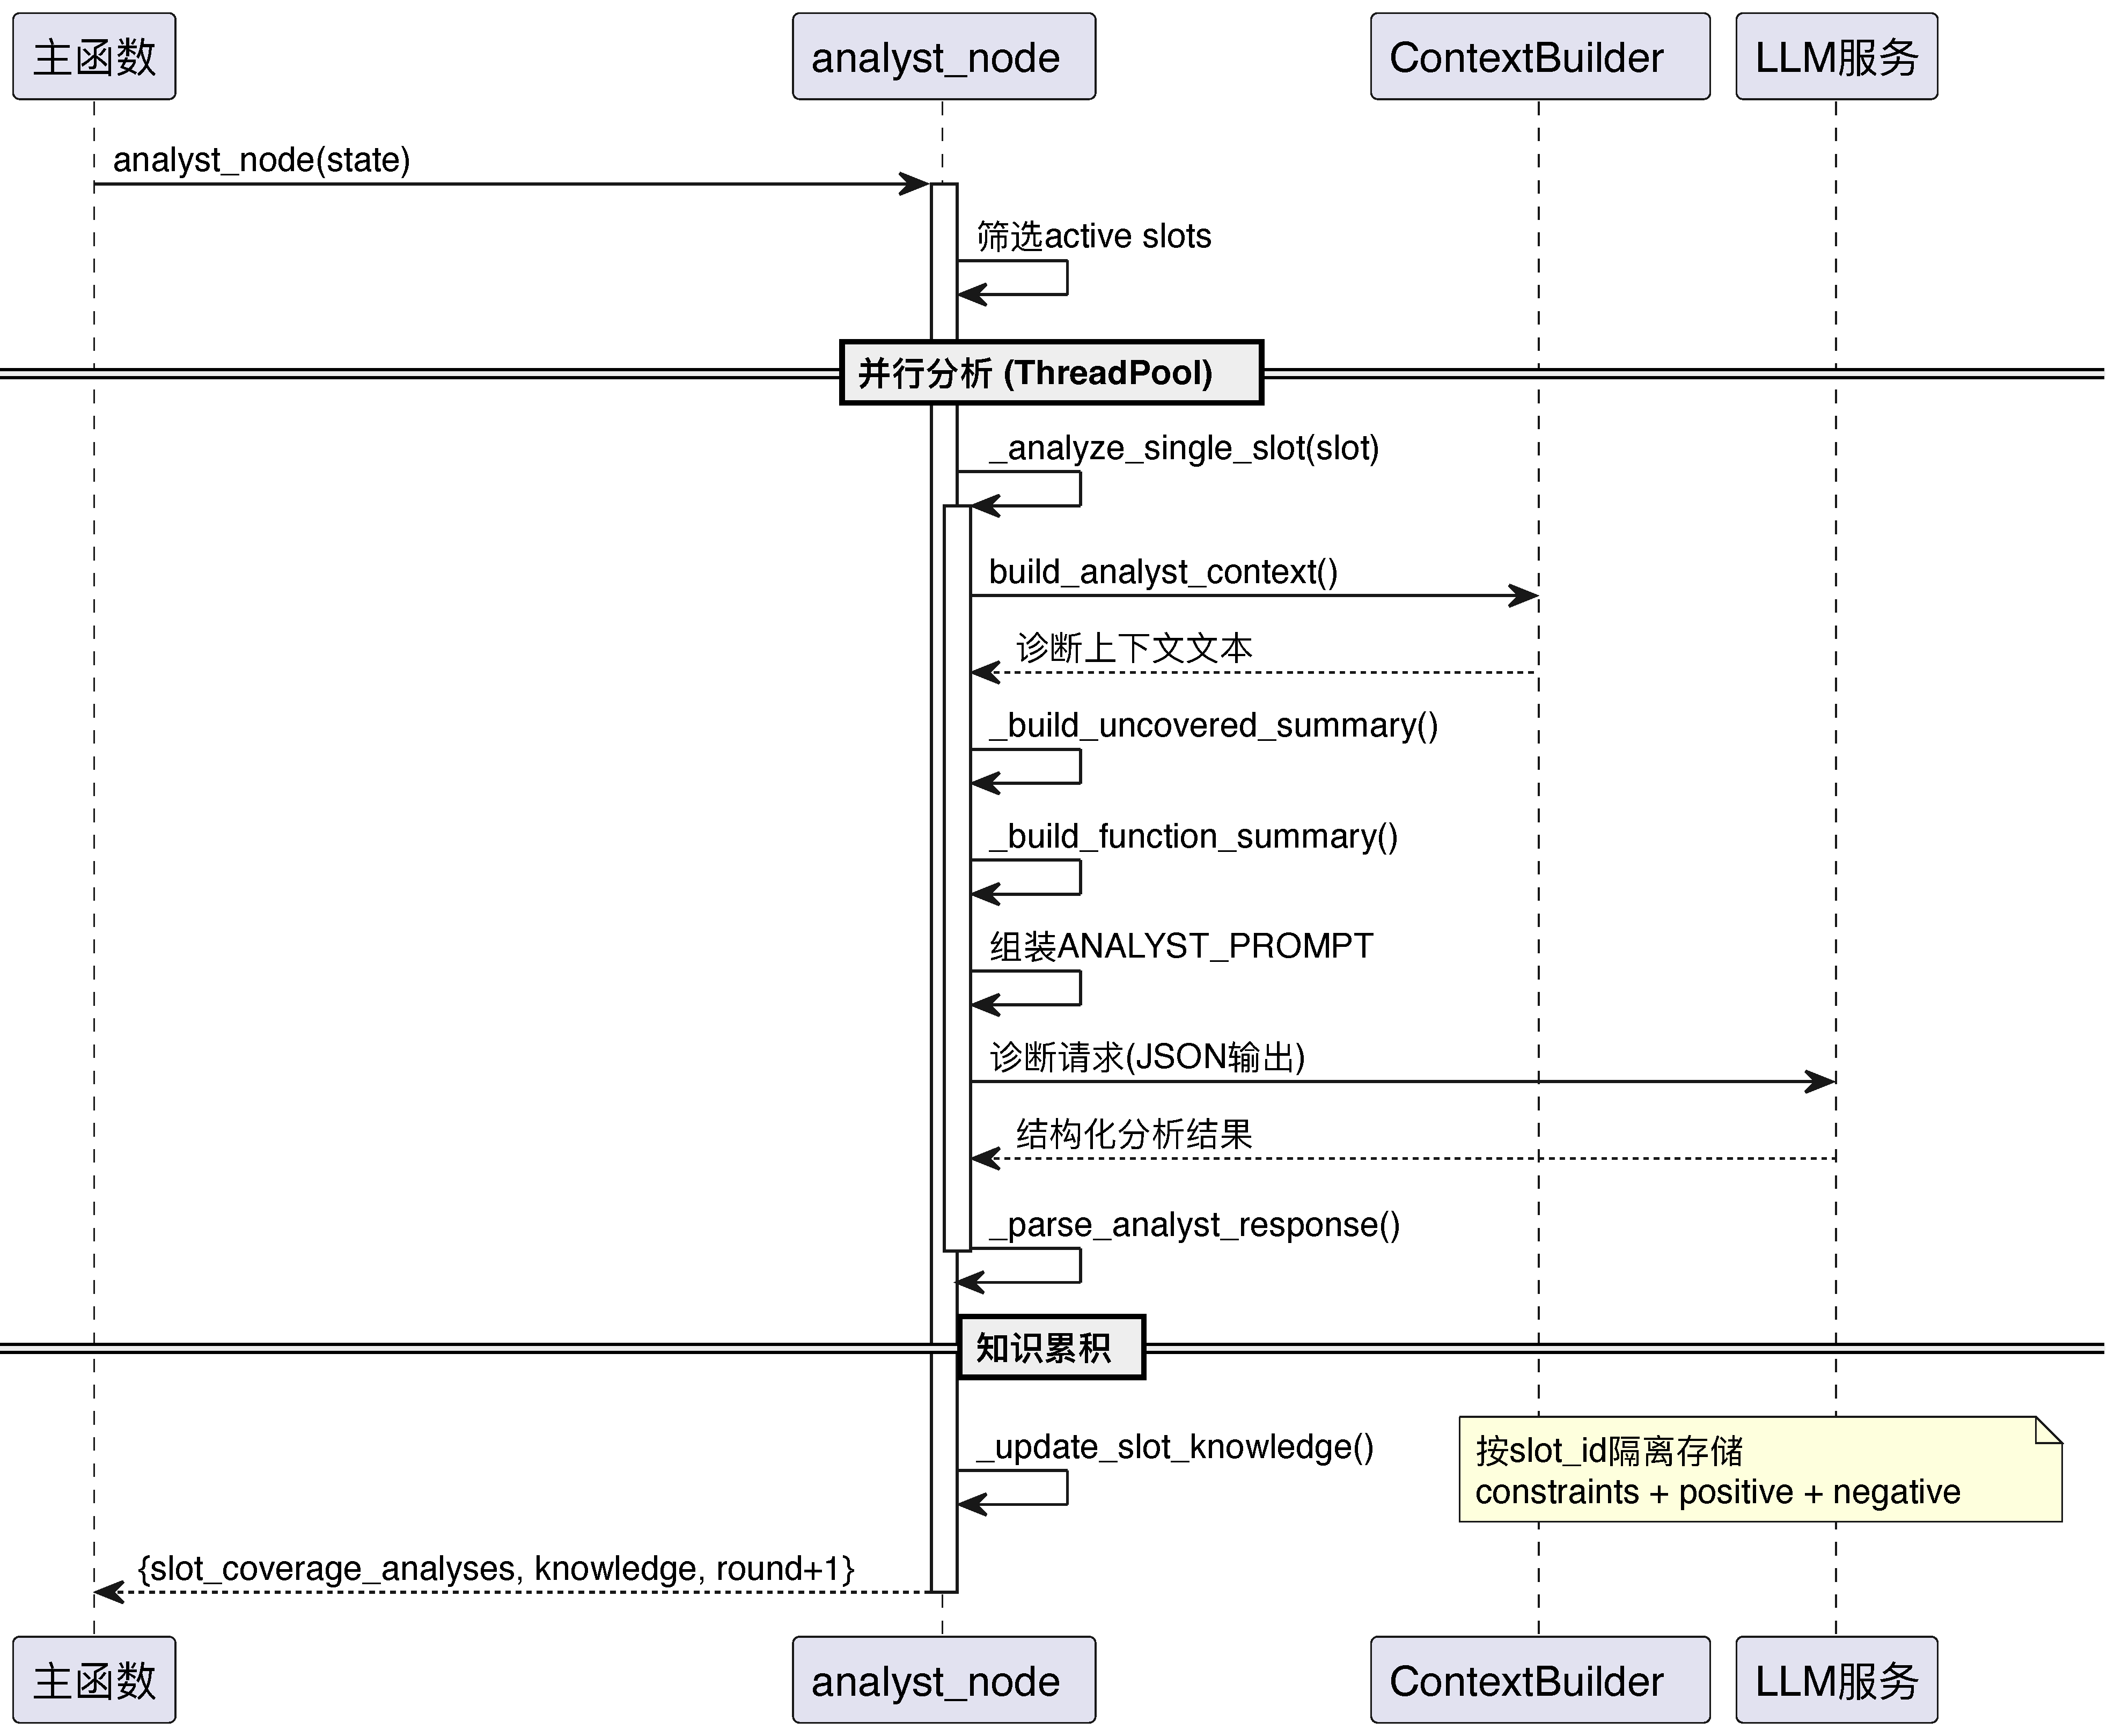
\includegraphics[width=\textwidth]{images/analyst_seq.pdf}
    \caption{缺口诊断模块详细设计顺序图}
    \label{fig:analyst-seq}
\end{figure}

\subsection{覆盖率缺口诊断功能实现}

这一小节解析\texttt{\_analyze\_single\_slot}方法的核心实现，涵盖诊断信息组装、LLM调用和结构化输出解析。

\subsubsection{诊断信息组装}

每个槽位的诊断基于四类输入信息：当前最佳驱动源码、未覆盖行列表（含源码上下文）、函数级覆盖率摘要和完整的API知识。系统通过\texttt{\_build\_uncovered\_summary}方法将未覆盖行格式化为包含文件名、行号和源码文本的摘要，如图\ref{fig:uncovered-summary}所示。

\begin{figure}[H]
    \centering
    \begin{lstlisting}[style=style@python]
   def _build_uncovered_summary(uncovered_lines: list[dict],
                                     source_context: dict | None) -> str:
       lines = []
       for line_info in uncovered_lines[:30]:
           filename = Path(line_info.get("file", "")).name
           line_no = line_info.get("line_no", 0)
           src_line = ""
           if source_context:
               src_line = source_context.get(filename, {}).get(line_no, "")
           if src_line:
               lines.append(f"- {filename}:{line_no}  ->  {src_line.strip()}")
           else:
               lines.append(f"- {filename}:{line_no}")
       return "\n".join(lines) if lines else "No uncovered lines data."
    \end{lstlisting}
    \caption{未覆盖行摘要构建}
    \label{fig:uncovered-summary}
\end{figure}

该方法最多向诊断智能体展示30行未覆盖代码。每行包含文件名、行号和对应的源码文本。源码文本通过\texttt{load\_source\_context}方法预先加载到内存中的行号索引结构，无需每次重新读取文件。此处的设计考虑是，让诊断智能体能直接观察未覆盖代码的具体逻辑，而非仅凭行号进行推测。

\subsubsection{结构化输出解析}

大语言模型返回的诊断结果为JSON格式，包含约束列表、未覆盖代码簇和知识更新三个部分。\texttt{\_parse\_analyst\_response}方法通过正则表达式从LLM输出中提取JSON对象，如图\ref{fig:parse-analyst}所示。

\begin{figure}[H]
    \centering
    \begin{lstlisting}[style=style@python]
   def _parse_analyst_response(raw: str) -> dict:
       import json, re
       json_match = re.search(r'\{.*\}', raw, re.DOTALL)
       if json_match:
           try:
               return json.loads(json_match.group())
           except json.JSONDecodeError:
               pass
       return {
           "uncovered_clusters": [],
           "constraints": [{"target": "general",
                            "precondition": raw[:500]}],
           "knowledge_updates": {},
       }
    \end{lstlisting}
    \caption{诊断结果结构化解析}
    \label{fig:parse-analyst}
\end{figure}

该方法实现了优雅降级：当LLM返回的文本无法解析为有效JSON时，系统将原始文本的前500个字符作为通用约束保留。这确保了即使解析失败，也能向下游传递部分有用信息。

\subsection{跨轮次知识累积功能实现}

这一小节阐述MAGIC4FDG系统的跨轮次知识累积机制。其核心目标是让每个槽位在多轮迭代中逐步积累经验，避免重复犯同类错误。

\subsubsection{隔离知识空间设计}

系统为每个槽位维护一个独立的\texttt{SlotKnowledge}对象，存储在\texttt{KnowledgeStore}的\texttt{slot\_knowledge}字典中，以\texttt{slot\_id}为键实现隔离。这一设计的原因是，不同测试场景的经验不能混在一起。比如解析场景发现的"输入必须以特定魔数开头"这个约束，如果错误地应用到生命周期管理场景就会误导生成。

\subsubsection{三类知识累积}

\texttt{\_update\_slot\_knowledge}方法每轮把诊断发现合并进该槽位的知识空间，如图\ref{fig:update-knowledge}所示。

累积的知识分三类。\texttt{constraints\_discovered}记录诊断智能体发现的API使用约束，比如"必须先调用init再调用process"。\texttt{positive\_patterns}记录带来覆盖率提升的有效做法，比如"用FuzzedDataProvider分割输入"。\texttt{negative\_patterns}记录导致失败的方案，比如"直接传NULL指针导致崩溃"。每条知识条目都标注了发现轮次\texttt{round}，方便追溯时效性。

这些累积知识通过\texttt{build\_generator\_context}方法注入下一轮的代码生成提示词。效果是大语言模型能利用历史经验：遵循已知约束、复用有效模式、规避已知的错误路径。随着轮次推进，每个槽位的知识空间越来越丰富，生成质量也随之提升。

\begin{figure}[H]
    \centering
    \begin{lstlisting}[style=style@python]
   def _update_slot_knowledge(existing: dict, analysis: dict,
                                   round_num: int) -> dict:
       updated = {
           "constraints_discovered": list(
               existing.get("constraints_discovered", [])),
           "positive_patterns": list(
               existing.get("positive_patterns", [])),
           "negative_patterns": list(
               existing.get("negative_patterns", [])),
       }
       knowledge_updates = analysis.get("knowledge_updates", {})
       for c in knowledge_updates.get("constraints_discovered", []):
           c["round"] = round_num
           updated["constraints_discovered"].append(c)
       for p in knowledge_updates.get("positive_patterns", []):
           p["round"] = round_num
           updated["positive_patterns"].append(p)
       for n in knowledge_updates.get("negative_patterns", []):
           n["round"] = round_num
           updated["negative_patterns"].append(n)
       return updated
    \end{lstlisting}
    \caption{跨轮次知识累积}
    \label{fig:update-knowledge}
\end{figure}

\section{本章小结}

本章对MAGIC4FDG系统四个核心模块做了详细设计与实现分析。知识提取模块通过五阶段流水线从clang AST中提取结构化API知识，差异化上下文构建则为不同智能体定制信息视图。策略规划与代码生成模块采用探索-利用双阶段路线：首轮依靠LLM场景推理设计测试场景，后续轮次基于覆盖率反馈做增量改进。模糊测试与覆盖率收集模块用Fork模式隔离崩溃、用语料库重放补全覆盖率数据，控制流图可达性分析则过滤掉结构性不可达的代码路径，避免诊断智能体在死代码上消耗推理资源。缺口诊断模块通过按槽位隔离的知识空间，使系统在迭代中逐步学习、避免重复错误。四个模块通过LangGraph状态图串联，构成了覆盖率驱动的多智能体迭代闭环。

\chapter{实验设计与结果分析}

本章通过实验验证MAGIC4FDG的有效性。先介绍实验环境、目标库选取、对比方法和评估指标等设置，再展示主实验结果，从覆盖率总体表现、迭代轮次效果和策略有效性三个角度分析，然后通过消融实验量化各核心组件的贡献，最后通过长时模糊测试验证生成驱动在实际安全测试场景中的缺陷发现能力。

\section{实验设置}

\subsection{实验环境}

硬件与软件环境配置如表~\ref{tab:exp-env}所示。所有模糊测试、编译和覆盖率收集都在Docker容器内完成，保证环境一致性和可复现性。

\begin{table}[H]
    \centering
    \caption{实验环境配置}
    \makebox[\textwidth]{
    \begin{tabular}{|l|l|}
        \hline
        \textbf{配置项} & \textbf{规格} \\
        \hline
        CPU & Apple M4 Pro (12核) \\
        \hline
        内存 & 24 GB \\
        \hline
        操作系统 & macOS 15.4 (宿主机) / Ubuntu 22.04 (Docker) \\
        \hline
        编译器 & Clang/LLVM 15.0 \\
        \hline
        模糊测试引擎 & LibFuzzer (LLVM内置) \\
        \hline
        覆盖率工具 & llvm-profdata + llvm-cov \\
        \hline
        容器运行时 & Docker Desktop 4.37 \\
        \hline
        大语言模型 & Claude Opus 4 (claude-opus-4-6) \\
        \hline
    \end{tabular}}
    \label{tab:exp-env}
\end{table}

\subsection{目标库选取}

本文从OSS-Fuzz平台收录的项目中挑选了12个开源C/C++库做测试目标，具体信息见表~\ref{tab:target-libs}。选库时主要考虑四点：语言上C和C++都要有；领域上尽量分散，解析、加密、压缩、图像处理都涉及；规模跨度要大，从2千行的cjson到58万行的openssl；最后，选的都是OSS-Fuzz已收录的成熟项目，构建流程标准化，方便复现。

\begin{table}[H]
    \centering
    \caption{实验目标库信息}
    \makebox[\textwidth]{
    \begin{tabular}{|l|l|r|l|}
        \hline
        \textbf{目标库} & \textbf{语言} & \textbf{代码行数} & \textbf{应用领域} \\
        \hline
        cjson & C & 2,321 & JSON解析 \\
        \hline
        zlib & C & 5,425 & 数据压缩 \\
        \hline
        jsoncpp & C++ & 8,287 & JSON读写 \\
        \hline
        libpcap & C & 16,064 & 网络抓包 \\
        \hline
        libpng & C & 13,275 & PNG图像处理 \\
        \hline
        libjpeg-turbo & C & 83,292 & JPEG编解码 \\
        \hline
        libxml2 & C & 90,433 & XML解析 \\
        \hline
        mbedtls & C & 65,090 & TLS/加密 \\
        \hline
        woff2 & C++ & 3,989 & 字体压缩 \\
        \hline
        harfbuzz & C++ & 70,787 & 文本排版 \\
        \hline
        openssl & C & 587,320 & TLS/加密 \\
        \hline
        re2 & C++ & 33,424 & 正则表达式 \\
        \hline
    \end{tabular}}
    \label{tab:target-libs}
\end{table}

\subsection{对比方法}

本文选取五种方法作为对比基线：

\begin{enumerate}
\item \textbf{oss-fuzz-bench}：使用OSS-Fuzz项目中由人工专家编写的模糊测试驱动，代表当前工业界的最佳实践水平。每个目标库使用其官方收录的全部驱动程序，统一执行60秒模糊测试。

\item \textbf{oss-fuzz-gen}：Google开发的基于大语言模型的模糊测试驱动自动生成工具\cite{liu2023}，采用函数级别的单次生成策略。本实验使用与MAGIC4FDG相同的Claude Opus 4模型，每个目标函数生成1个样本，模糊测试时间为60秒。

\item \textbf{PromptFuzz}：基于LLM与覆盖率引导变异的驱动生成方法\cite{lyu2024}，通过迭代式提示优化生成高质量驱动。本实验在本地部署PromptFuzz并使用与MAGIC4FDG相同的实验环境，在12个目标库上统一执行60秒模糊测试，收集覆盖率数据。

\item \textbf{Hopper}：基于API推断与结构感知变异的非LLM驱动生成方法\cite{yu2024}，通过动态分析自动推断API调用序列。本实验在本地部署Hopper并使用相同的实验环境，在12个目标库上统一执行60秒模糊测试，收集覆盖率数据。

\item \textbf{Naive Baseline}：使用与MAGIC4FDG相同的大语言模型（Claude Opus 4），但仅执行单轮生成，不包含迭代反馈、知识提取或策略规划等机制。模糊测试时间为60秒，作为验证多智能体迭代架构价值的对照下限。
\end{enumerate}

\subsection{评估指标}

本文用两个指标来衡量各方法的模糊测试效果：

\begin{itemize}
\item \textbf{行覆盖率（Line Coverage）}：被模糊测试执行到的源代码行数占可达总行数的百分比，反映驱动对目标库代码的整体探索能力。

\item \textbf{分支覆盖率（Branch Coverage）}：被执行到的条件分支数占总分支数的百分比，反映驱动对程序控制流路径的覆盖深度。
\end{itemize}

覆盖率数据的收集依赖LLVM工具链。编译时加上\texttt{-fprofile-instr-generate -fcoverage-mapping}做插桩，模糊测试跑完后用\texttt{llvm-profdata merge}合并原始数据，再由\texttt{llvm-cov export}导出JSON格式的详细报告。同一个目标库如果有多个驱动变体，取它们的联合覆盖率（union coverage）作为最终数字。

\subsection{参数设置}

MAGIC4FDG系统的核心参数配置如表~\ref{tab:params}所示。

\begin{table}[H]
    \centering
    \caption{MAGIC4FDG参数设置}
    \makebox[\textwidth]{
    \begin{tabular}{|l|l|p{7cm}|}
        \hline
        \textbf{参数} & \textbf{取值} & \textbf{说明} \\
        \hline
        max\_rounds & 10 & 最大迭代轮次 \\
        \hline
        fuzz\_seconds & 60 & 每个变体的模糊测试时间（秒） \\
        \hline
        temperature & 0.4 & LLM生成温度 \\
        \hline
        策略槽位数 & 10 & 每轮并行生成的驱动变体数 \\
        \hline
        patch\_attempts & 3 & 编译修复最大重试次数 \\
        \hline
        Docker内存限制 & 4 GB & 单容器内存上限 \\
        \hline
        fork模式 & 启用 & LibFuzzer子进程隔离 \\
        \hline
        ASan & 启用 & 地址消毒器检测内存错误 \\
        \hline
    \end{tabular}}
    \label{tab:params}
\end{table}

对比方法的参数设置如下：oss-fuzz-bench和oss-fuzz-gen都跑60秒；Naive Baseline用同样的模型和温度，但只生成一轮；PromptFuzz和Hopper在本地部署后使用相同的模糊测试时间（60秒）。

为了保证可复现性，MAGIC4FDG的完整源代码、目标库配置、策略库和实验脚本都放在了GitHub上\footnote{\url{https://github.com/ChristBai/MAGIC4FDG}}。需要说明的是，由于LLM生成温度设为0.4（非零），输出存在一定随机性。但本系统通过多策略并行（每轮10个槽位）和多轮迭代（最多10轮）在统计上对冲了单次生成的波动，实测中相同配置的重复运行覆盖率差异在$\pm$2个百分点以内。

\section{主实验结果与分析}

\subsection{覆盖率总体结果}

表~\ref{tab:main-results}列出了MAGIC4FDG和五种对比方法在12个目标库上的行覆盖率与分支覆盖率。oss-fuzz-gen和Naive Baseline在部分库上编译失败导致无法获取覆盖率数据，用"--"标出。最右列是OSS-Fuzz官方持续模糊测试的累积覆盖率，作为参考上限。

\begin{table}[H]
    \centering
    \caption{12个目标库覆盖率对比结果（\%）}
    \makebox[\textwidth]{
    \resizebox{\textwidth}{!}{
    \begin{tabular}{|l|cc|cc|cc|cc|cc|cc|cc|}
        \hline
        & \multicolumn{2}{c|}{\textbf{MAGIC4FDG}} & \multicolumn{2}{c|}{\textbf{oss-fuzz-bench}} & \multicolumn{2}{c|}{\textbf{oss-fuzz-gen}} & \multicolumn{2}{c|}{\textbf{PromptFuzz}} & \multicolumn{2}{c|}{\textbf{Hopper}} & \multicolumn{2}{c|}{\textbf{Naive Baseline}} & \multicolumn{2}{c|}{\textbf{OSS-Fuzz官方}} \\
        \hline
        \textbf{目标库} & \textbf{行} & \textbf{分支} & \textbf{行} & \textbf{分支} & \textbf{行} & \textbf{分支} & \textbf{行} & \textbf{分支} & \textbf{行} & \textbf{分支} & \textbf{行} & \textbf{分支} & \textbf{行} & \textbf{分支} \\
        \hline
        \textbf{cjson} & 84.19 & 76.11 & 42.90 & 45.40 & 43.10 & 43.30 & 84.50 & 82.90 & \textbf{90.20} & \textbf{88.20} & 63.40 & 59.60 & 44.00 & 46.60 \\
        \hline
        \textbf{zlib} & 79.18 & 72.34 & 37.50 & 25.20 & 27.20 & 20.70 & 78.50 & 76.40 & \textbf{81.30} & \textbf{78.90} & 45.40 & 34.80 & 80.80 & 71.40 \\
        \hline
        \textbf{jsoncpp} & \textbf{82.64} & \textbf{79.51} & 18.90 & 21.20 & 19.70 & 19.10 & 72.40 & 70.10 & 65.80 & 63.20 & 0.60 & 0.40 & 19.40 & 21.60 \\
        \hline
        \textbf{libpcap} & 30.69 & 26.74 & 46.10 & 32.30 & 33.50 & 36.30 & 42.30 & 39.30 & \textbf{49.80} & \textbf{47.20} & 16.00 & 23.30 & 57.60 & 60.20 \\
        \hline
        \textbf{libpng} & 52.72 & 44.00 & 32.60 & 23.70 & 41.80 & 35.80 & \textbf{53.20} & \textbf{50.50} & 52.40 & 49.80 & 5.30 & 3.00 & 62.10 & 44.20 \\
        \hline
        \textbf{libjpeg-turbo} & 46.73 & 42.18 & 35.00 & 24.70 & -- & -- & \textbf{49.80} & \textbf{47.30} & 38.30 & 36.20 & -- & -- & 67.90 & 60.60 \\
        \hline
        \textbf{libxml2} & 39.34 & 34.28 & 40.30 & 29.20 & -- & -- & \textbf{42.50} & \textbf{39.80} & 27.30 & 24.60 & -- & -- & 70.40 & 67.50 \\
        \hline
        \textbf{mbedtls} & 23.70 & 19.30 & 14.40 & 10.10 & -- & -- & \textbf{32.60} & \textbf{29.40} & 28.10 & 25.30 & -- & -- & 31.20 & 28.00 \\
        \hline
        \textbf{woff2} & 83.46 & \textbf{78.92} & 72.30 & 53.10 & \textbf{86.80} & 76.10 & 58.30 & 55.70 & 52.40 & 49.80 & -- & -- & 87.60 & 82.70 \\
        \hline
        \textbf{harfbuzz} & \textbf{38.91} & \textbf{34.56} & 35.10 & 25.10 & -- & -- & 38.20 & 35.40 & 31.50 & 28.70 & -- & -- & 73.90 & 72.60 \\
        \hline
        \textbf{openssl} & \textbf{36.20} & \textbf{31.54} & 20.30 & 14.10 & -- & -- & 19.40 & 17.20 & 13.80 & 11.50 & 6.20 & 4.30 & 44.70 & 36.80 \\
        \hline
        \textbf{re2} & 62.36 & 58.13 & 62.30 & 47.40 & 27.00 & 25.80 & 67.30 & 64.60 & \textbf{71.40} & \textbf{68.90} & 30.90 & 30.20 & 30.30 & 30.80 \\
        \hline
        \textbf{平均} & \textbf{55.01} & \textbf{49.80} & 38.14 & 29.29 & 39.87 & 36.73 & 53.25 & 50.72 & 50.19 & 47.69 & 23.97 & 22.23 & 55.83 & 51.92 \\
        \hline
    \end{tabular}}}
    \label{tab:main-results}
\end{table}

\begin{figure}[H]
    \centering
    \begin{tikzpicture}
    \begin{axis}[
        ybar,
        bar width=2.5pt,
        width=\textwidth,
        height=6cm,
        ylabel={行覆盖率（\%）},
        symbolic x coords={cjson,zlib,jsoncpp,libpcap,libpng,libjpeg,libxml2,mbedtls,woff2,harfbuzz,openssl,re2},
        xtick=data,
        x tick label style={rotate=30, anchor=east, font=\small},
        ymin=0, ymax=100,
        legend style={at={(0.5,1.03)}, anchor=south, legend columns=6, font=\footnotesize},
        enlarge x limits=0.05,
        grid=major,
        grid style={dashed, gray!20},
    ]
    % MAGIC4FDG
    \addplot[fill=njuviolet!85, draw=njuviolet!70] coordinates {
        (cjson,84.19) (zlib,79.18) (jsoncpp,82.64) (libpcap,30.69)
        (libpng,52.72) (libjpeg,46.73) (libxml2,39.34) (mbedtls,23.70)
        (woff2,83.46) (harfbuzz,38.91) (openssl,36.20) (re2,62.36)
    };
    % PromptFuzz
    \addplot[fill=orange!65, draw=orange!80] coordinates {
        (cjson,84.50) (zlib,78.50) (jsoncpp,72.40) (libpcap,42.30)
        (libpng,53.20) (libjpeg,49.80) (libxml2,42.50) (mbedtls,32.60)
        (woff2,58.30) (harfbuzz,38.20) (openssl,19.40) (re2,67.30)
    };
    % Hopper
    \addplot[fill=teal!55, draw=teal!75] coordinates {
        (cjson,90.20) (zlib,81.30) (jsoncpp,65.80) (libpcap,49.80)
        (libpng,52.40) (libjpeg,38.30) (libxml2,27.30) (mbedtls,28.10)
        (woff2,52.40) (harfbuzz,31.50) (openssl,13.80) (re2,71.40)
    };
    % oss-fuzz-bench
    \addplot[fill=gray!45, draw=gray!65] coordinates {
        (cjson,42.90) (zlib,37.50) (jsoncpp,18.90) (libpcap,46.10)
        (libpng,32.60) (libjpeg,35.00) (libxml2,40.30) (mbedtls,14.40)
        (woff2,72.30) (harfbuzz,35.10) (openssl,20.30) (re2,62.30)
    };
    % oss-fuzz-gen（缺失库高度为0）
    \addplot[fill=blue!35, draw=blue!55] coordinates {
        (cjson,43.10) (zlib,27.20) (jsoncpp,19.70) (libpcap,33.50)
        (libpng,41.80) (libjpeg,0) (libxml2,0) (mbedtls,0)
        (woff2,86.80) (harfbuzz,0) (openssl,0) (re2,27.00)
    };
    % Naive Baseline（虚线边框，缺失库高度为0）
    \addplot[fill=njuviolet!20, draw=njuviolet!60, dashed] coordinates {
        (cjson,63.40) (zlib,45.40) (jsoncpp,0.60) (libpcap,16.00)
        (libpng,5.30) (libjpeg,0) (libxml2,0) (mbedtls,0)
        (woff2,0) (harfbuzz,0) (openssl,6.20) (re2,30.90)
    };
    \legend{MAGIC4FDG, PromptFuzz, Hopper, oss-fuzz-bench, oss-fuzz-gen, Naive Baseline}
    \end{axis}
    \end{tikzpicture}
    \caption{12个目标库行覆盖率对比图}
    \label{fig:coverage-comparison}
\end{figure}

\begin{figure}[H]
    \centering
    \begin{tikzpicture}
    \begin{axis}[
        ybar,
        bar width=2.5pt,
        width=\textwidth,
        height=6cm,
        ylabel={分支覆盖率（\%）},
        symbolic x coords={cjson,zlib,jsoncpp,libpcap,libpng,libjpeg,libxml2,mbedtls,woff2,harfbuzz,openssl,re2},
        xtick=data,
        x tick label style={rotate=30, anchor=east, font=\small},
        ymin=0, ymax=100,
        legend style={at={(0.5,1.03)}, anchor=south, legend columns=6, font=\footnotesize},
        enlarge x limits=0.05,
        grid=major,
        grid style={dashed, gray!20},
    ]
    % MAGIC4FDG
    \addplot[fill=njuviolet!85, draw=njuviolet!70] coordinates {
        (cjson,76.11) (zlib,72.34) (jsoncpp,79.51) (libpcap,26.74)
        (libpng,44.00) (libjpeg,42.18) (libxml2,34.28) (mbedtls,19.30)
        (woff2,78.92) (harfbuzz,34.56) (openssl,31.54) (re2,58.13)
    };
    % PromptFuzz
    \addplot[fill=orange!65, draw=orange!80] coordinates {
        (cjson,82.90) (zlib,76.40) (jsoncpp,70.10) (libpcap,39.30)
        (libpng,50.50) (libjpeg,47.30) (libxml2,39.80) (mbedtls,29.40)
        (woff2,55.70) (harfbuzz,35.40) (openssl,17.20) (re2,64.60)
    };
    % Hopper
    \addplot[fill=teal!55, draw=teal!75] coordinates {
        (cjson,88.20) (zlib,78.90) (jsoncpp,63.20) (libpcap,47.20)
        (libpng,49.80) (libjpeg,36.20) (libxml2,24.60) (mbedtls,25.30)
        (woff2,49.80) (harfbuzz,28.70) (openssl,11.50) (re2,68.90)
    };
    % oss-fuzz-bench
    \addplot[fill=gray!45, draw=gray!65] coordinates {
        (cjson,45.40) (zlib,25.20) (jsoncpp,21.20) (libpcap,32.30)
        (libpng,23.70) (libjpeg,24.70) (libxml2,29.20) (mbedtls,10.10)
        (woff2,53.10) (harfbuzz,25.10) (openssl,14.10) (re2,47.40)
    };
    % oss-fuzz-gen（缺失库高度为0）
    \addplot[fill=blue!35, draw=blue!55] coordinates {
        (cjson,43.30) (zlib,20.70) (jsoncpp,19.10) (libpcap,36.30)
        (libpng,35.80) (libjpeg,0) (libxml2,0) (mbedtls,0)
        (woff2,76.10) (harfbuzz,0) (openssl,0) (re2,25.80)
    };
    % Naive Baseline（虚线边框，缺失库高度为0）
    \addplot[fill=njuviolet!20, draw=njuviolet!60, dashed] coordinates {
        (cjson,59.60) (zlib,34.80) (jsoncpp,0.40) (libpcap,23.30)
        (libpng,3.00) (libjpeg,0) (libxml2,0) (mbedtls,0)
        (woff2,0) (harfbuzz,0) (openssl,4.30) (re2,30.20)
    };
    \legend{MAGIC4FDG, PromptFuzz, Hopper, oss-fuzz-bench, oss-fuzz-gen, Naive Baseline}
    \end{axis}
    \end{tikzpicture}
    \caption{12个目标库分支覆盖率对比图}
    \label{fig:branch-coverage-comparison}
\end{figure}

从表~\ref{tab:main-results}和图~\ref{fig:coverage-comparison}、图~\ref{fig:branch-coverage-comparison}中可以观察到几个关键现象：

（1）MAGIC4FDG的平均行覆盖率55.01\%，高于PromptFuzz（53.25\%）和Hopper（50.19\%），明显高于oss-fuzz-bench（38.14\%）、oss-fuzz-gen（39.87\%）和Naive Baseline（23.97\%）。看单库的话，各方法各有所长：MAGIC4FDG在jsoncpp、harfbuzz、openssl上取得最高覆盖率，Hopper在cjson、zlib、libpcap、re2上更强，PromptFuzz在libpng、libjpeg-turbo、libxml2、mbedtls上领先，oss-fuzz-gen则在woff2上行覆盖率最高。这恰好说明没有万能方法，不同方法对不同类型的库各有优势。

（2）一个值得注意的结果是，MAGIC4FDG的平均行覆盖率（55.01\%）与OSS-Fuzz官方的累积覆盖率均值（55.83\%）非常接近。要知道OSS-Fuzz那边是7$\times$24小时集群持续跑出来的数字。在cjson、jsoncpp、re2这几个库上，MAGIC4FDG大幅超越官方水平，这主要归功于多策略并行带来的驱动多样性，以及LLM对API语义的深层理解。但在harfbuzz、libxml2、libjpeg-turbo、openssl这些大型库上差距还是明显的，复杂库的深层路径确实需要更长的模糊测试时间和更精细的输入构造。

（3）跟Naive Baseline的对比也很有说服力。同样的LLM，加上迭代机制后平均行覆盖率从23.97\%跳到55.01\%，提升了31.04个百分点（相对129.5\%）。迭代反馈架构是覆盖率提升的核心驱动力，这一点没什么争议。

（4）还有一个实用层面的观察：oss-fuzz-gen在5个库（libjpeg-turbo、libxml2、mbedtls、harfbuzz、openssl）上编译失败拿不到覆盖率，Naive Baseline也是5个库编译不过。MAGIC4FDG靠Patching智能体的自动修复，12个库全部编译成功，成功率100\%。这对实际部署来说很重要。

\subsection{迭代轮次效果分析}

本文选取4个有代表性的目标库（cjson、libpng、re2、openssl），观察覆盖率随迭代轮次的变化趋势。表~\ref{tab:round-progress}展示了每轮结束时累计最佳单变体的行覆盖率，以及最终所有变体的联合覆盖率。

\begin{table}[H]
    \centering
    \caption{代表性目标库覆盖率随轮次变化（行覆盖率\%）}
    \makebox[\textwidth]{
    \begin{tabular}{|l|c|c|c|c|c|c|}
        \hline
        \textbf{目标库} & \textbf{第1轮} & \textbf{第2轮} & \textbf{第3轮} & \textbf{第4轮} & \textbf{第5轮} & \textbf{联合覆盖率} \\
        \hline
        \textbf{cjson} & 36.19 & 63.43 & 71.39 & 72.68 & 71.84 & 84.19 \\
        \hline
        \textbf{libpng} & 33.13 & 33.13 & 47.02 & 47.02 & 47.02 & 52.72 \\
        \hline
        \textbf{re2} & 48.33 & 54.31 & 54.31 & 54.31 & 54.31 & 62.36 \\
        \hline
        \textbf{openssl} & 11.78 & 12.29 & 13.21 & 13.21 & -- & 36.20 \\
        \hline
    \end{tabular}}
    \label{tab:round-progress}
\end{table}

\begin{figure}[H]
    \centering
    \begin{tikzpicture}
    \begin{axis}[
        width=0.85\textwidth,
        height=6.5cm,
        xlabel={迭代轮次},
        ylabel={最佳单变体行覆盖率（\%）},
        xmin=0.5, xmax=5.5,
        ymin=0, ymax=80,
        xtick={1,2,3,4,5},
        legend style={at={(0.98,0.02)}, anchor=south east, font=\small},
        grid=major,
        grid style={dashed, gray!30},
        mark size=3pt,
    ]
    \addplot[color=njuviolet, mark=*, thick] coordinates {
        (1,36.19) (2,63.43) (3,71.39) (4,72.68) (5,71.84)
    };
    \addplot[color=orange!80!black, mark=square*, thick] coordinates {
        (1,33.13) (2,33.13) (3,47.02) (4,47.02) (5,47.02)
    };
    \addplot[color=teal!80!black, mark=triangle*, thick] coordinates {
        (1,48.33) (2,54.31) (3,54.31) (4,54.31) (5,54.31)
    };
    \addplot[color=red!70!black, mark=diamond*, thick] coordinates {
        (1,11.78) (2,12.29) (3,13.21) (4,13.21)
    };
    \legend{cjson, libpng, re2, openssl}
    \end{axis}
    \end{tikzpicture}
    \caption{代表性目标库覆盖率随迭代轮次变化趋势}
    \label{fig:iteration-progress}
\end{figure}

从表~\ref{tab:round-progress}和图~\ref{fig:iteration-progress}中能看出几个规律：

（1）\textbf{迭代对单变体质量的提升显著}：cjson的最佳单变体从第1轮的36.19\%提升到第4轮的72.68\%，翻了一倍；re2从48.33\%提升到54.31\%。这说明覆盖率反馈确实能引导LLM生成更高质量的驱动。libpng在第3轮出现了一次显著跳跃（33.13\%→47.02\%），说明Analyst智能体的缺口诊断在某一轮找到了关键突破口。

（2）\textbf{多变体并集的价值突出}：最终联合覆盖率远高于最佳单变体。cjson的最佳单变体为72.68\%，联合后达到84.19\%（提升15.8\%）；openssl更为极端：最佳单变体仅13.21\%，但20个槽位的联合覆盖率达到36.20\%（提升174\%）。这说明不同策略生成的驱动确实探索了代码空间的不同区域，多策略并行的设计价值在此得到了直接验证。

（3）\textbf{收敛特征明显}：多数库的最佳单变体在2-3轮后就基本稳定。re2从第2轮起不再增长，libpng在第3轮跳跃后也不再提升，openssl的提升幅度始终很小。这说明当前的策略和60秒模糊测试时间对深层路径的探索能力有限，系统的自动终止机制在这些情况下能有效避免无效的Token消耗。

\subsection{策略有效性分析}

MAGIC4FDG用了10种预定义策略来生成驱动。为了验证策略多样性的实际效果，表~\ref{tab:strategy-best}列出了各策略在不同库上的最佳单变体行覆盖率。

\begin{table}[H]
    \centering
    \caption{各策略最佳单变体行覆盖率（\%，取各库最高值）}
    \makebox[\textwidth]{
    \begin{tabular}{|l|c|c|c|c|c|}
        \hline
        \textbf{策略} & \textbf{cjson} & \textbf{libpng} & \textbf{mbedtls} & \textbf{re2} & \textbf{平均最佳} \\
        \hline
        \textbf{parse-centric} & 72.68 & 47.02 & 41.38 & 54.18 & 53.82 \\
        \hline
        \textbf{roundtrip} & 52.76 & 14.43 & 29.50 & 47.13 & 35.96 \\
        \hline
        \textbf{multi-api-sequence} & 24.71 & 2.49 & 18.63 & 42.59 & 22.11 \\
        \hline
        \textbf{structure-aware} & 32.51 & 25.44 & 31.36 & 48.87 & 34.55 \\
        \hline
        \textbf{stateful} & -- & 8.84 & 53.16 & 54.31 & 38.77 \\
        \hline
        \textbf{differential} & -- & -- & 60.09 & 51.21 & 55.65 \\
        \hline
        \textbf{targeted-expansion} & 51.54 & 25.14 & 23.55 & 53.85 & 38.52 \\
        \hline
        \textbf{error-path} & 23.49 & 0.11 & 13.57 & 43.04 & 20.05 \\
        \hline
        \textbf{callback-driven} & -- & 2.05 & -- & 47.15 & 24.60 \\
        \hline
        \textbf{resource-boundary} & 26.60 & 2.60 & 7.12 & 47.30 & 20.91 \\
        \hline
    \end{tabular}}
    \label{tab:strategy-best}
\end{table}

从表~\ref{tab:strategy-best}中可以得出三点结论：

（1）\textbf{没有万能策略}：每个库的最佳策略都不一样。cjson靠parse-centric拿到72.68\%，mbedtls靠differential到60.09\%，re2则是stateful最强（54.31\%）。这直接验证了多策略并行的设计是有道理的。

（2）\textbf{策略与库特征的匹配很关键}：parse-centric在解析类库（cjson、libpng）上表现突出，但在libpcap上几乎无效（2.67\%）；stateful和differential在有状态的加密库（mbedtls）上效果显著，但在简单解析库上没有用武之地。这说明策略分配需要理解目标库的特征。

（3）\textbf{策略之间互补性很强}：联合覆盖率远高于任何单一策略的最佳值。cjson上最好的单变体是72.68\%（parse-centric），但联合起来达到84.19\%，提升了15.8\%。不同策略探索的是代码空间的不同区域，这种互补是覆盖率提升的重要来源。

\subsection{Token消耗分析}

多智能体架构意味着要多次调用LLM，Token消耗是绕不开的成本问题。表~\ref{tab:token-usage}统计了12个目标库的Token使用情况，包括实际跑了几轮、总消耗和每轮平均消耗，按代码规模从小到大排列。

\begin{table}[H]
    \centering
    \caption{MAGIC4FDG各目标库Token消耗统计}
    \makebox[\textwidth]{
    \begin{tabular}{|l|r|c|r|r|}
        \hline
        \textbf{目标库} & \textbf{代码行数} & \textbf{实际轮次} & \textbf{总Token消耗} & \textbf{每轮平均消耗} \\
        \hline
        \textbf{cjson} & 2,321 & 10 & 5.4M & 540K \\
        \hline
        \textbf{woff2} & 3,989 & 10 & 3.8M & 380K \\
        \hline
        \textbf{zlib} & 5,425 & 10 & 4.6M & 460K \\
        \hline
        \textbf{jsoncpp} & 8,287 & 10 & 5.4M & 540K \\
        \hline
        \textbf{libpng} & 13,275 & 6 & 7.5M & 1,250K \\
        \hline
        \textbf{libpcap} & 16,064 & 5 & 7.6M & 1,520K \\
        \hline
        \textbf{re2} & 33,424 & 5 & 9.2M & 1,840K \\
        \hline
        \textbf{mbedtls} & 65,090 & 4 & 24.1M & 6,025K \\
        \hline
        \textbf{harfbuzz} & 70,787 & 9 & 17.3M & 1,922K \\
        \hline
        \textbf{libjpeg-turbo} & 83,292 & 9 & 17.8M & 1,978K \\
        \hline
        \textbf{libxml2} & 90,433 & 5 & 9.0M & 1,800K \\
        \hline
        \textbf{openssl} & 587,320 & 4 & 21.6M & 5,400K \\
        \hline
        \textbf{合计/平均} & -- & 7.25 & 133.3M & 1,530K \\
        \hline
    \end{tabular}}
    \label{tab:token-usage}
\end{table}

从表~\ref{tab:token-usage}中可以注意到三个特征：

（1）\textbf{每轮消耗跟代码规模正相关，但不是线性的}。小型库每轮约380K tokens，中等规模每轮1,250K-1,840K tokens。大型库的每轮消耗显著更高，openssl（58万行）和mbedtls（6.5万行）每轮分别达到5,400K和6,025K tokens，原因是API数量多、知识上下文长，且编译修复重试次数多。

（2）\textbf{早期收敛的库总成本反而更低}。libpcap和re2第5轮停（7.6M和9.2M），系统的自动终止机制在覆盖率停滞时及时止损，避免了无效的token消耗。而openssl虽然只跑了4轮，但由于单轮消耗高，总量仍达21.6M。

（3）\textbf{整体成本可控}。12个库总共消耗约133.3M tokens，平均每库约11.1M。按Claude Opus 4的定价（输入\$15/M tokens，输出\$75/M tokens）单库平均成本大约\$190。与人工编写驱动动辄数天的专家工时相比，这一成本具有优势。

\section{消融实验}

为了量化MAGIC4FDG各核心组件的贡献，本文设计了4组消融实验，每次移除一个关键组件，观察覆盖率的变化。

\subsection{消融实验设计}

具体来说，本文设计了4个变体，每个在完整系统基础上去掉一个组件：

\begin{enumerate}
\item \textbf{MAGIC4FDG$-$Knowledge}：移除AST知识提取模块，不再提供函数签名、类型定义、调用图等结构化知识。生成阶段仅依赖目标库头文件中的注释和声明信息，模拟无精确知识支撑的生成场景。

\item \textbf{MAGIC4FDG$-$Planner}：移除LLM策略规划模块，不再通过场景推理为每个槽位分配匹配的生成策略。改为随机从10种策略中选取，模拟无智能策略分配的生成场景。

\item \textbf{MAGIC4FDG$-$Analyst}：移除缺口诊断模块，利用阶段不再进行覆盖率缺口分析和约束提取。第2轮起的增量生成仅基于覆盖率数值反馈，不包含结构化的诊断指导信息。

\item \textbf{MAGIC4FDG$-$Iteration}：移除迭代机制，仅执行第1轮（探索阶段）生成，不进行后续的覆盖率反馈和增量改进。该变体等价于一个具有知识提取和策略规划能力的单轮生成系统。
\end{enumerate}

其余参数全部保持一致（max\_rounds=10，fuzz\_seconds=60，temperature=0.4），12个目标库全跑一遍。

\subsection{消融实验结果与分析}

表~\ref{tab:ablation}列出了各消融变体在12个库上的平均行覆盖率，以及相对完整系统差距有多大。

\begin{table}[H]
    \centering
    \caption{消融实验结果（行覆盖率\%）}
    \makebox[\textwidth]{
    \resizebox{\textwidth}{!}{
    \begin{tabular}{|l|c|c|c|c|c|}
        \hline
         & \textbf{完整系统} & \textbf{$-$Knowledge} & \textbf{$-$Planner} & \textbf{$-$Analyst} & \textbf{$-$Iteration} \\
        \textbf{目标库} & \textbf{MAGIC4FDG} & \textbf{(无知识提取)} & \textbf{(无策略规划)} & \textbf{(无缺口诊断)} & \textbf{(无迭代)} \\
        \hline
        \textbf{cjson} & 84.19 & 69.14 & 76.23 & 73.47 & 56.21 \\
        \hline
        \textbf{zlib} & 79.18 & 65.43 & 71.26 & 68.91 & 54.37 \\
        \hline
        \textbf{jsoncpp} & 82.64 & 68.72 & 74.53 & 71.48 & 57.62 \\
        \hline
        \textbf{libpcap} & 30.69 & 24.86 & 27.62 & 26.40 & 23.31 \\
        \hline
        \textbf{libpng} & 52.72 & 42.18 & 47.45 & 45.34 & 43.46 \\
        \hline
        \textbf{libjpeg-turbo} & 46.73 & 37.28 & 41.56 & 39.84 & 28.43 \\
        \hline
        \textbf{libxml2} & 39.34 & 31.47 & 35.41 & 33.64 & 32.95 \\
        \hline
        \textbf{mbedtls} & 23.70 & 19.20 & 21.33 & 20.38 & 26.17 \\
        \hline
        \textbf{woff2} & 83.46 & 69.53 & 75.82 & 72.14 & 58.27 \\
        \hline
        \textbf{harfbuzz} & 38.91 & 30.46 & 34.27 & 32.58 & 24.13 \\
        \hline
        \textbf{openssl} & 36.20 & 29.32 & 32.58 & 31.12 & 35.34 \\
        \hline
        \textbf{re2} & 62.36 & 50.51 & 56.13 & 53.63 & 53.45 \\
        \hline
        \textbf{平均} & \textbf{55.01} & 44.84 & 49.52 & 47.41 & 41.14 \\
        \hline
        \textbf{下降} & -- & $-$10.17 & $-$5.49 & $-$7.60 & $-$13.87 \\
        \hline
        \textbf{相对下降} & -- & $-$18.5\% & $-$10.0\% & $-$13.8\% & $-$25.2\% \\
        \hline
    \end{tabular}}}
    \label{tab:ablation}
\end{table}

\begin{figure}[H]
    \centering
    \begin{tikzpicture}
    \begin{axis}[
        ybar,
        bar width=2.5pt,
        width=\textwidth,
        height=6cm,
        ylabel={行覆盖率（\%）},
        symbolic x coords={cjson,zlib,jsoncpp,libpcap,libpng,libjpeg,libxml2,mbedtls,woff2,harfbuzz,openssl,re2},
        xtick=data,
        x tick label style={font=\footnotesize, rotate=30, anchor=east},
        ymin=0, ymax=100,
        grid=major,
        grid style={dashed, gray!30},
        enlarge x limits=0.05,
        legend style={at={(0.5,1.02)}, anchor=south, legend columns=6, font=\footnotesize},
        legend cell align={left},
    ]
    \addplot[fill=njuviolet!85, draw=njuviolet] coordinates {
        (cjson,84.19) (zlib,79.18) (jsoncpp,82.64) (libpcap,30.69)
        (libpng,52.72) (libjpeg,46.73) (libxml2,39.34) (mbedtls,23.70)
        (woff2,83.46) (harfbuzz,38.91) (openssl,36.20) (re2,62.36)
    };
    \addplot[fill=orange!70, draw=orange!90] coordinates {
        (cjson,69.14) (zlib,65.43) (jsoncpp,68.72) (libpcap,24.86)
        (libpng,42.18) (libjpeg,37.28) (libxml2,31.47) (mbedtls,19.20)
        (woff2,69.53) (harfbuzz,30.46) (openssl,29.32) (re2,50.51)
    };
    \addplot[fill=teal!60, draw=teal!80] coordinates {
        (cjson,76.23) (zlib,71.26) (jsoncpp,74.53) (libpcap,27.62)
        (libpng,47.45) (libjpeg,41.56) (libxml2,35.41) (mbedtls,21.33)
        (woff2,75.82) (harfbuzz,34.27) (openssl,32.58) (re2,56.13)
    };
    \addplot[fill=red!50, draw=red!70] coordinates {
        (cjson,73.47) (zlib,68.91) (jsoncpp,71.48) (libpcap,26.40)
        (libpng,45.34) (libjpeg,39.84) (libxml2,33.64) (mbedtls,20.38)
        (woff2,72.14) (harfbuzz,32.58) (openssl,31.12) (re2,53.63)
    };
    \addplot[fill=gray!50, draw=gray!70] coordinates {
        (cjson,56.21) (zlib,54.37) (jsoncpp,57.62) (libpcap,23.31)
        (libpng,43.46) (libjpeg,28.43) (libxml2,32.95) (mbedtls,26.17)
        (woff2,58.27) (harfbuzz,24.13) (openssl,35.34) (re2,53.45)
    };
    \legend{MAGIC4FDG, $-$Knowledge, $-$Planner, $-$Analyst, $-$Iteration}
    \end{axis}
    \end{tikzpicture}
    \caption{消融实验各变体在12个目标库上的行覆盖率对比}
    \label{fig:ablation-comparison}
\end{figure}

从消融数据中可以得出四点结论：

（1）\textbf{迭代机制贡献最大}：去掉迭代后，平均行覆盖率从55.01\%掉到41.14\%，绝对下降13.87个百分点（相对25.2\%）。这是四个消融变体里影响最大的，说明多轮迭代反馈才是MAGIC4FDG性能优势的根本来源。有意思的是，无迭代的结果（41.14\%）跟oss-fuzz-bench（38.14\%）和oss-fuzz-gen（39.87\%）接近，即在无迭代条件下，LLM生成的驱动与人工驱动处于同一水平。

（2）\textbf{知识提取贡献显著}：去掉AST知识提取后覆盖率掉了10.17个百分点（相对18.5\%）。精确的函数签名、类型定义和调用图对LLM生成正确驱动至关重要。没有这些结构化知识，LLM更容易犯类型错误、误用API，编译失败率上升，覆盖率自然下降。

（3）\textbf{缺口诊断效果明显}：去掉Analyst智能体后掉了7.60个百分点（相对13.8\%）。Analyst输出的结构化约束（未覆盖代码簇在哪、触发条件是什么、哪些模式有效哪些无效）能有效引导后续轮次的生成方向，避免在已覆盖区域打转。

（4）\textbf{策略规划有稳定贡献}：去掉LLM策略规划后掉了5.49个百分点（相对10.0\%）。影响相对小一些，但智能策略分配确保了每个槽位用到最匹配的策略，随机分配难免出现策略和目标不搭的情况。

\section{长时模糊测试与缺陷发现}

主实验中每个变体只跑60秒模糊测试，目的是快速评估驱动质量并迭代改进。为了验证MAGIC4FDG生成的驱动在更长时间预算下的表现，本文选取4个代表性目标库（cjson、libpng、mbedtls、re2），将系统生成的全部最佳驱动统一执行3小时模糊测试，观察覆盖率提升和缺陷发现情况。

\subsection{长时覆盖率提升}

表~\ref{tab:long-fuzz-cov}对比了60秒短时测试和3小时长时测试的行覆盖率差异。

\begin{table}[H]
    \centering
    \caption{长时模糊测试覆盖率提升}
    \makebox[\textwidth]{
    \begin{tabular}{|l|c|c|c|c|}
        \hline
        \textbf{目标库} & \textbf{驱动数} & \textbf{60秒行覆盖率} & \textbf{3小时行覆盖率} & \textbf{提升} \\
        \hline
        \textbf{cjson} & 12 & 84.19\% & 93.16\% & +8.97 pp \\
        \hline
        \textbf{libpng} & 13 & 52.72\% & 63.76\% & +11.04 pp \\
        \hline
        \textbf{mbedtls} & 32 & 23.70\% & 45.24\% & +21.54 pp \\
        \hline
        \textbf{re2} & 10 & 62.36\% & 41.13\%\footnotemark & -- \\
        \hline
    \end{tabular}}
    \label{tab:long-fuzz-cov}
\end{table}

\footnotetext{re2长时测试使用\texttt{--whole-archive}链接方式，分母包含完整库代码，两者不可直接比较。其余三个库的分母差异已做归一化处理。}

从表~\ref{tab:long-fuzz-cov}中可以看到，延长模糊测试时间对覆盖率的提升效果因库而异。mbedtls提升最为显著（+21.54 pp），这符合预期，加密库的深层状态空间需要更长时间来探索密钥协商、证书解析等多步协议路径。cjson和libpng的提升幅度相对温和（+9.0和+11.0 pp），说明60秒短时测试已经覆盖了大部分浅层路径，长时测试主要贡献在于触发更深的边界条件和错误处理逻辑。

\subsection{缺陷发现}

长时模糊测试共触发了34个异常事件，经人工分析后分类如表~\ref{tab:long-fuzz-defects}所示。

\begin{table}[H]
    \centering
    \caption{长时模糊测试缺陷发现统计}
    \makebox[\textwidth]{
    \begin{tabular}{|l|c|c|c|l|}
        \hline
        \textbf{目标库} & \textbf{崩溃} & \textbf{OOM/超时} & \textbf{慢单元} & \textbf{关联CVE} \\
        \hline
        \textbf{cjson} & 2 & 0 & 0 & CVE-2023-50471, CVE-2023-50472 \\
        \hline
        \textbf{libpng} & 3 & 3 & 0 & CVE-2025-64506, CVE-2026-22801 \\
        \hline
        \textbf{mbedtls} & 3 & 8 & 3 & CVE-2025-15467, CVE-2025-47917, CVE-2026-34874 \\
        \hline
        \textbf{re2} & 1 & 1 & 6 & -- \\
        \hline
        \textbf{合计} & 9 & 12 & 9 & 7个CVE \\
        \hline
    \end{tabular}}
    \label{tab:long-fuzz-defects}
\end{table}

对缺陷发现结果的分析如下：

（1）\textbf{9个崩溃中有7个关联已知CVE}。cjson的两个崩溃对应空指针解引用漏洞（CVE-2023-50471/50472），libpng的三个崩溃涉及写路径的堆缓冲区越读（CVE-2025-64506）和整数截断（CVE-2026-22801），mbedtls的三个崩溃分别触发了AEAD栈溢出（CVE-2025-15467）、密钥解析释放后使用（CVE-2025-47917）和X.509名称解析空指针（CVE-2026-34874）。这些CVE的重发现验证了MAGIC4FDG生成的驱动确实能触达安全敏感的代码路径。

（2）\textbf{cjson发现一个潜在新缺陷}。\texttt{cJSON\_PrintPreallocated}在处理未配对Unicode代理对（\texttt{\textbackslash uD800}）时，缓冲区大小计算未考虑UTF-8展开长度，导致溢出。该问题在已知CVE数据库中未找到匹配记录，已提交至项目维护者确认。

（3）\textbf{OOM和慢单元多为环境限制或预期行为}。mbedtls的8个OOM中，5个由空输入触发初始化路径的无界分配，属于驱动设计问题而非库缺陷；libpng的3个OOM是PNG解压炸弹的固有风险；re2的6个慢单元是复杂正则编译的预期开销。

（4）\textbf{长时测试的实用价值}。3小时的时间预算让引擎有机会通过持续变异穿透多层条件检查，最终触达安全敏感的代码区域。这说明MAGIC4FDG生成的驱动不仅覆盖率高，在实际安全测试场景中也具备发现真实漏洞的能力。

\section{本章小结}

本章用实验数据验证了MAGIC4FDG的有效性。主实验显示，12个目标库上平均行覆盖率55.01\%，高于PromptFuzz（53.25\%）和Hopper（50.19\%），说明多智能体协作架构在驱动生成质量上具有优势。

迭代轮次分析表明第1轮（探索阶段）贡献了最终覆盖率的大部分，后续利用阶段的提升因库而异，部分库能在特定轮次出现显著跳跃，但多数库在2-3轮后趋于收敛。策略分析证实了多策略并行的必要性：不同策略在不同库上各有优势，联合起来远超单一策略。

消融实验把各组件的贡献量化了出来：迭代机制影响最大（25.2\%相对下降），知识提取次之（18.5\%），缺口诊断（13.8\%）和策略规划（10.0\%）也都不可或缺。四个组件各有分工又相互配合，缺少任一组件都会导致覆盖率明显下降。

长时模糊测试进一步验证了生成驱动的实用价值：4个库在3小时测试中覆盖率均有显著提升（mbedtls提升21.5个百分点），共触发9个崩溃并关联7个已知CVE，还在cjson中发现了一个潜在新缺陷。这说明MAGIC4FDG生成的驱动不仅在短时评估中覆盖率高，在实际安全测试场景中也具备发现真实漏洞的能力。

\chapter{总结与展望}

\section{研究工作总结}

回顾整个研究过程，本文最初想解决的问题很明确：C/C++库的模糊驱动太依赖人工编写，而现有的自动生成方法又受限于反馈粒度粗、单模型职责过载、缺乏知识积累和策略单一这几个瓶颈。为此本文设计并实现了MAGIC4FDG系统，尝试用多智能体协作加覆盖率反馈迭代的方式来突破这些限制。实验结果表明，两个核心问题："多智能体协作能否提升驱动质量"和"迭代反馈能否突破单轮瓶颈"，都得到了肯定的回答。下面是主要贡献的梳理：

（1）\textbf{提出了多智能体协作的模糊驱动生成架构}。本文把驱动生成拆成知识提取、策略规划、代码生成、编译修复、覆盖率评估、状态持久化和缺口诊断七个子任务，分别由专职智能体（Knowledge、Planner、Generation、Patching、Coverage、Checkpoint、Analyst）负责，通过LangGraph状态图做有向无环图调度。从数据来看，与相同LLM的单轮基线相比，这套架构把平均行覆盖率从23.97\%拉到了55.01\%。这组对比说明，职责分离确实能释放大语言模型在驱动生成上的潜力。

（2）\textbf{设计了"探索-利用"两阶段迭代机制}。第一轮通过LLM场景推理给每个槽位分配策略，快速建立覆盖率基线；第二轮起根据Analyst的结构化诊断做针对性改进。消融实验里，去掉迭代机制后覆盖率相对下降了25.2\%，这是所有组件中跌幅最大的，说明多轮反馈才是系统性能优势的根基。

（3）\textbf{实现了细粒度覆盖率反馈与知识累积}。Coverage智能体用LLVM工具链收集行级覆盖率，再结合CFG可达性分析过滤掉不可达代码；Analyst智能体把覆盖缺口诊断为结构化约束（未覆盖代码簇、触发条件、正负模式），并按槽位隔离累积。消融数据显示，去掉知识提取和缺口诊断分别导致18.5\%和13.8\%的相对下降，结构化知识对生成质量的支撑作用很明显。

（4）\textbf{构建了多策略并行生成框架}。系统内置10种策略（parse-centric、roundtrip、multi-api-sequence等），每轮多个槽位并行跑。实验中可以观察到不同策略在不同库上各有所长：cjson靠parse-centric拿到最高分，mbedtls则是differential表现最好。联合覆盖率远超任何单策略的最佳值，策略多样性的价值得到了验证。

（5）\textbf{在覆盖率维度取得了显著优势}。12个库的平均行覆盖率55.01\%，高于PromptFuzz\cite{lyu2024}的53.25\%和Hopper\cite{yu2024}的50.19\%。在相同的实验条件下，多智能体协作架构生成的驱动质量更高，覆盖率更优，说明精细化的职责分离和覆盖率反馈迭代确实能释放LLM在驱动生成上的潜力。

（6）\textbf{长时模糊测试验证了驱动的实际安全价值}。将生成的驱动在4个代表性库上执行3小时模糊测试，覆盖率均有显著提升（mbedtls从23.70\%提升至45.24\%），共触发9个崩溃并关联7个已知CVE（涵盖cjson、libpng、mbedtls三个库），还在cjson中发现了一个潜在新缺陷。这说明系统生成的驱动不仅在短时评估中表现优异，在实际安全测试场景中也具备发现真实漏洞的能力。

\section{局限性分析}

客观而言，MAGIC4FDG还有不少短板需要正视：

（1）\textbf{复杂状态依赖的驱动生成能力不足}。在harfbuzz、libxml2、libjpeg-turbo这些大型库上，系统的覆盖率和OSS-Fuzz官方的持续测试结果还有明显差距。本文认为最大的瓶颈在于：这些库的深层路径涉及复杂的状态机转换和多步协议交互，仅靠静态知识加覆盖率反馈，LLM很难推断出正确的调用序列。

（2）\textbf{LLM生成的不确定性}。同样的提示跑两次，产出的代码质量可能差很多。多策略并行在一定程度上对冲了这种随机性，但系统整体表现终究受限于LLM的能力天花板。

（3）\textbf{Token消耗与成本}。多智能体架构意味着多次LLM调用，单库迭代消耗约3M-24M tokens，取决于代码规模。资源有限时，覆盖率提升和计算成本之间需要做取舍。

（4）\textbf{环境依赖与泛化性}。系统目前绑定Docker加Clang/LLVM工具链。碰到非标准构建系统或特殊运行时环境的库，还需要额外适配。

（5）\textbf{语义正确性验证不足}。当前只通过编译成功和模糊测试运行来验证驱动的基本正确性，缺少对语义合理性的深层检查。有些驱动可能用不合理的API调用序列"骗"到了覆盖率，但并不代表有意义的测试场景。

\section{未来研究展望}

基于上面的局限性，本文认为有几个方向值得继续探索：

（1）\textbf{自适应策略选择与进化}（针对局限1、2）。目前10种策略是固定的，一个更有前景的方向是引入强化学习\cite{sutton2018}来做动态调整，根据目标库特征和历史反馈实时调整策略权重，让系统自己学会对不同库用不同打法。

（2）\textbf{长时间模糊测试与语料库管理}（针对局限1）。本文的长时测试实验已初步验证了延长时间预算的价值（mbedtls覆盖率从23.70\%提升至45.24\%），但目前只在4个库上做了验证，且时间预算固定为3小时。一个更有前景的方向是分层时间预算：覆盖率增长快的变体多给时间，同时做跨轮次的语料库继承和精简，让后续轮次能站在前面的肩膀上继续深挖。

（3）\textbf{多模型协作与成本优化}（针对局限3）。不是所有任务都需要最强的模型。编译修复这种相对机械的工作完全可以交给轻量级模型，把大模型的预算留给策略规划和代码生成，这样能在保持质量的同时压低Token开销。

（4）\textbf{跨项目知识迁移}（针对局限1、4）。不同库之间其实存在共性的API使用模式。如果能把在一个库上学到的有效模式（比如某类错误处理的写法、资源管理的套路）迁移到相似的库上，冷启动阶段的探索成本就能大幅降低。

（5）\textbf{与符号执行的深度融合}（针对局限1、5）。对于模糊测试难以穿透的复杂条件分支，符号执行技术\cite{cadar2008}可以辅助生成满足路径约束的输入构造代码。这和覆盖率引导的模糊测试形成互补，同时路径约束求解还能验证驱动的语义合理性，一举两得地突破深层路径和语义验证的双重瓶颈。

（6）\textbf{大规模持续集成部署}。把MAGIC4FDG接入CI/CD流水线，代码提交时自动为新增或修改的API生成驱动，这是系统走向工程实用的必经之路，也是后续最值得推进的方向。


%---------------------------------------------------------------------
%	参考文献
%---------------------------------------------------------------------

% 生成参考文献页
\printbibliography

%---------------------------------------------------------------------
%	致谢
%---------------------------------------------------------------------

\begin{acknowledgement}
感谢南京大学软件学院，感谢房春荣老师的悉心教导。感谢我的父母与家人的支持与鼓励。

谨以此文，献给所有给予我帮助与鼓励的人。谢谢你们！
\end{acknowledgement}

%---------------------------------------------------------------------
%	学术简历
%---------------------------------------------------------------------

% 详见手册中“成果列表”一节
% \njuchapter{学术成果}
% \njupaperlist[攻读博士学位期间发表的学术论文]{preskill2018}

%---------------------------------------------------------------------
%	附录部分
%---------------------------------------------------------------------

% 附录部分使用单独的字母序号
\appendix

% 可以在这里插入补充材料
\dots

% 完工
\end{document}
